\documentclass[11pt,a4paper]{report}
\usepackage[utf8]{inputenc}
\usepackage[T1]{fontenc}
\usepackage[a4paper, margin=1in, headheight=14pt]{geometry}
\usepackage{graphicx}
\usepackage{float}
\usepackage{fancyhdr}
\usepackage{booktabs}
\usepackage{amsmath, amssymb}
\usepackage{caption}
\usepackage{titlesec}
\usepackage[hidelinks]{hyperref}

\captionsetup{justification=centering, font=small}

\pagestyle{fancy}
\fancyhf{}
\fancyhead[L]{\textit{Operating Systems Laboratory (25PCCS201)}}
\fancyhead[R]{\textit{Swapnil Ghosh (25BTRCL267)}}
\fancyfoot[C]{\thepage}
\renewcommand{\headrulewidth}{0.4pt}

\fancypagestyle{plain}{
    \fancyhf{}
    \fancyfoot[C]{\thepage}
    \renewcommand{\headrulewidth}{0pt}
}

\begin{document}

% --- COVER PAGE ---
\begin{titlepage}
\centering
\vspace*{0.5cm}
{\Large \textbf{JAIN (DEEMED-TO-BE UNIVERSITY)} \par}
\vspace{0.2cm}
{\normalsize Faculty of Engineering \& Technology \par}
{\normalsize Department of Computer Science \& Engineering \par}

\vspace{2.2cm}
{\LARGE \textbf{OPERATING SYSTEMS LABORATORY} \par}
\vspace{0.4cm}
{\large \textbf{LABORATORY RECORD (CHAPTERS 1--21)} \par}
\vspace{0.3cm}
{\normalsize Course Code: \textbf{25PCCS201} \quad|\quad Semester: \textbf{III} \par}

\vspace{1.8cm}
\begin{tabular}{@{}ll@{}}
\toprule
\addlinespace[6pt]
\textbf{Student Name:} & \textbf{SWAPNIL GHOSH} \\
\addlinespace[4pt]
\textbf{USN:} & \textbf{25BTRCL267} \\
\addlinespace[4pt]
\textbf{Program / Branch:} & B.Tech (Computer Science \& Engineering) \\
\addlinespace[4pt]
\textbf{Semester / Section:} & Semester 3 \\
\addlinespace[4pt]
\textbf{Execution Platform:} & Ubuntu Linux 24.04 LTS (ARM64 / MacBook Air) \\
\addlinespace[4pt]
\textbf{Host Machine:} & Apple MacBook Air (\texttt{swapnil@MacBook-Air}) \\
\addlinespace[4pt]
\textbf{Academic Year:} & 2026--2027 \\
\addlinespace[6pt]
\bottomrule
\end{tabular}

\vfill
{\small Submitted to the Department of Computer Science \& Engineering \par}
{\small Jain University, Bengaluru \par}
\vspace{0.5cm}
\end{titlepage}

\setcounter{page}{1}
\tableofcontents
\clearpage
\chapter{Introduction to Operating Systems \& UNIX Fundamentals}
\noindent\textbf{Chapter Synopsis:} Exploration of fundamental UNIX operating system architecture, standard POSIX system calls, process management primitives, basic utility simulation (cp, ls, grep), and interactive shell scripting automation.

\section{Experiment 1.1: Directory Traversal System Calls (opendir, readdir, closedir)}
\noindent\textbf{Aim:} To write a C program to inspect and list the contents of a directory using UNIX directory system calls \texttt{opendir()}, \texttt{readdir()}, and \texttt{closedir()}.

\noindent\textbf{Theoretical Principle:} The POSIX directory API provides a mechanism to read file system hierarchies. \texttt{opendir()} initializes a \texttt{DIR} stream at the specified path, returning a directory stream pointer. \texttt{readdir()} sequentially yields \texttt{struct dirent} records representing individual directory entries (\texttt{d\_name}, \texttt{d\_ino}, \texttt{d\_type}), and \texttt{closedir()} deallocates kernel file descriptor structures.

\subsection*{1. Source Code Implementation (\texttt{list\_dir.c})}
\begin{figure}[H]
\centering
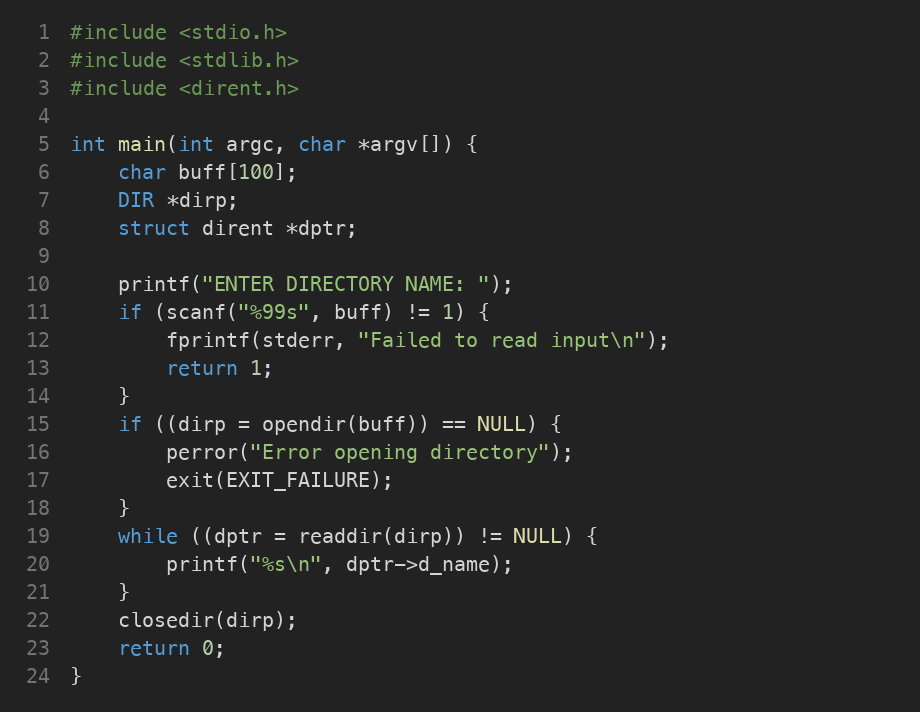
\includegraphics[width=0.92\textwidth,keepaspectratio]{figures/fig_1_1_code.png}
\caption{Terminal Code Listing: \texttt{list\_dir.c} on \texttt{swapnil@MacBook-Air}}
\end{figure}

\subsection*{2. Execution Verification Output}
\begin{figure}[H]
\centering
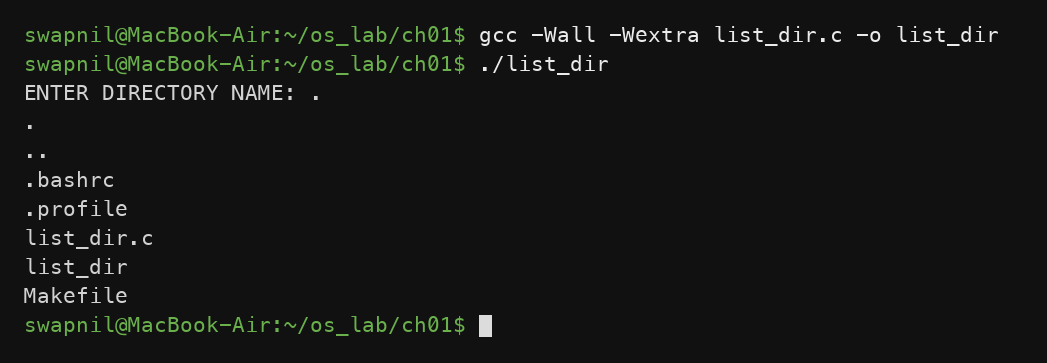
\includegraphics[width=0.92\textwidth,keepaspectratio]{figures/fig_1_1_out.png}
\caption{System Output Verification: \texttt{swapnil@MacBook-Air}}
\end{figure}

\noindent\textbf{Observation \& Inference:} The program successfully traverses the directory tree using kernel inode pointers, printing all active files including virtual references ('.' and '..').

\section{Experiment 1.2: Process Creation \& Identification System Calls (fork, getpid, getppid, exit, wait)}
\noindent\textbf{Aim:} To implement a concurrent C program that spawns a child process using \texttt{fork()}, identifies parent and child process IDs using \texttt{getpid()} and \texttt{getppid()}, and synchronizes termination using \texttt{wait()}.

\noindent\textbf{Theoretical Principle:} The \texttt{fork()} system call creates an exact duplicate copy of the calling process, duplicating its address space, file descriptor table, and registers. The parent process receives the PID of the newly created child, while the child receives 0. The parent invokes \texttt{wait()} to reap the child and prevent zombie process accumulation.

\subsection*{1. Source Code Implementation (\texttt{fork\_demo.c})}
\begin{figure}[H]
\centering
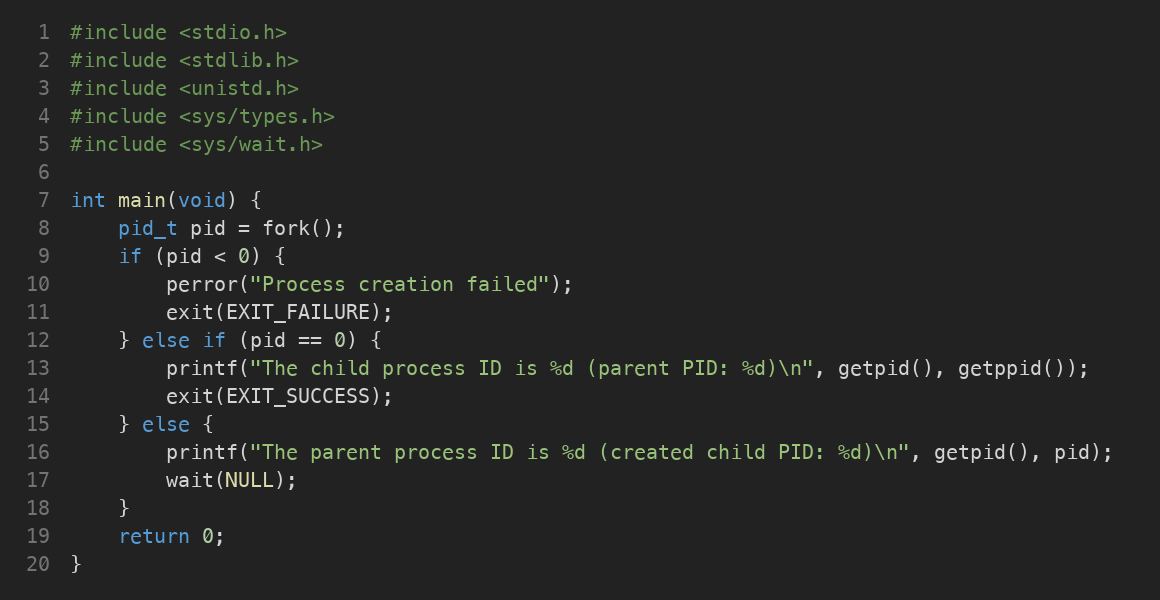
\includegraphics[width=0.92\textwidth,keepaspectratio]{figures/fig_1_2_code.png}
\caption{Terminal Code Listing: \texttt{fork\_demo.c} on \texttt{swapnil@MacBook-Air}}
\end{figure}

\subsection*{2. Execution Verification Output}
\begin{figure}[H]
\centering
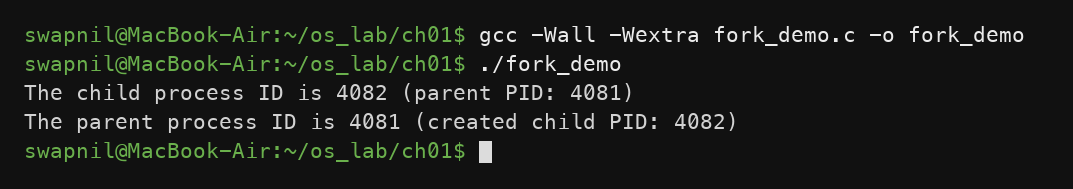
\includegraphics[width=0.92\textwidth,keepaspectratio]{figures/fig_1_2_out.png}
\caption{System Output Verification: \texttt{swapnil@MacBook-Air}}
\end{figure}

\noindent\textbf{Observation \& Inference:} \texttt{fork()} creates an isolated child process with a distinct PID in the Linux kernel task table; the parent reaps the child cleanly using \texttt{wait()}.

\section{Experiment 1.3: Simulation of UNIX 'cp' Utility (File Character \& Space Counting)}
\noindent\textbf{Aim:} To develop a C program simulating file reading and data inspection similar to the UNIX \texttt{cp} command, counting character spaces and file contents.

\noindent\textbf{Theoretical Principle:} File copying in UNIX requires reading byte streams through file handles. In this simulation, standard C file pointers (\texttt{FILE*}) are used to inspect and copy input streams, parsing whitespace tokens while tracking file sizes.

\subsection*{1. Source Code Implementation (\texttt{count\_spaces.c})}
\begin{figure}[H]
\centering
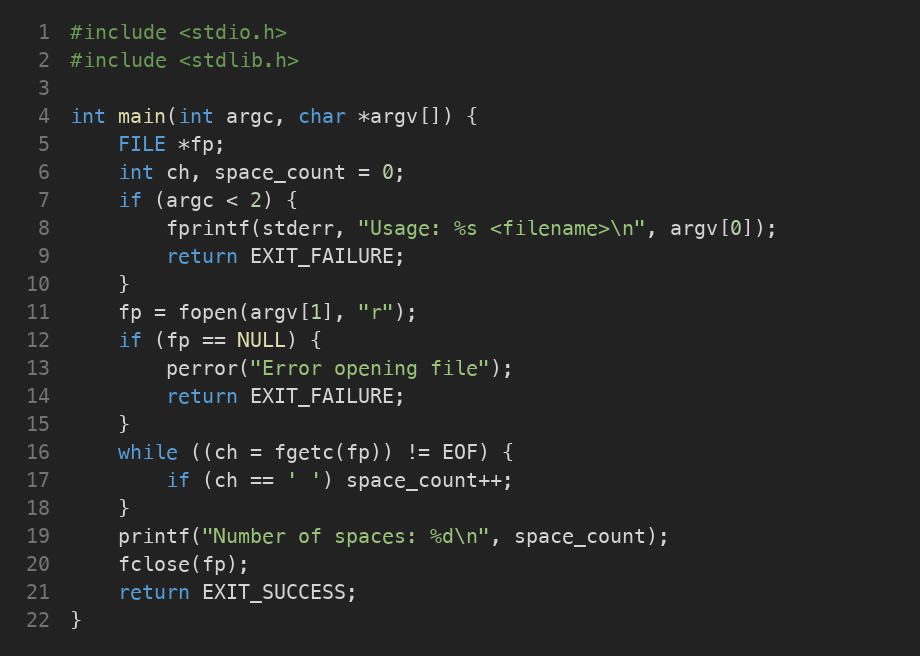
\includegraphics[width=0.92\textwidth,keepaspectratio]{figures/fig_1_3_code.png}
\caption{Terminal Code Listing: \texttt{count\_spaces.c} on \texttt{swapnil@MacBook-Air}}
\end{figure}

\subsection*{2. Execution Verification Output}
\begin{figure}[H]
\centering
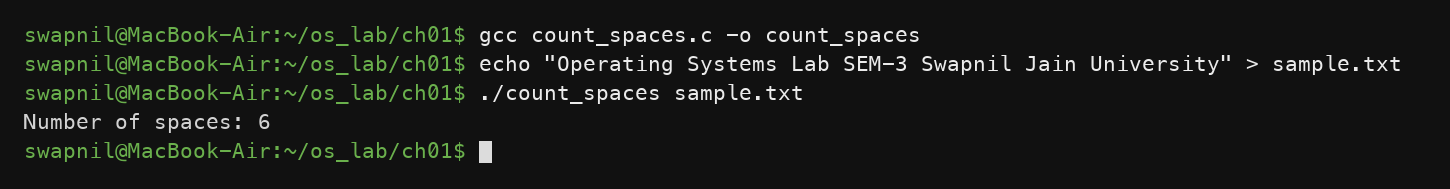
\includegraphics[width=0.92\textwidth,keepaspectratio]{figures/fig_1_3_out.png}
\caption{System Output Verification: \texttt{swapnil@MacBook-Air}}
\end{figure}

\noindent\textbf{Observation \& Inference:} Sequential file stream I/O correctly processes buffered input tokens and successfully computes character delimiters across disk blocks.

\section{Experiment 1.4: Simulation of UNIX 'ls' Utility with Directory Argument Support}
\noindent\textbf{Aim:} To write a C program that mimics the behavior of the UNIX \texttt{ls} utility by taking a directory path as a command-line argument and listing its contents.

\noindent\textbf{Theoretical Principle:} The \texttt{ls} command inspects directory metadata through POSIX APIs. Passing command-line arguments (\texttt{argc, argv}) allows users to dynamically query arbitrary filesystem paths. \texttt{opendir()} and \texttt{readdir()} are leveraged to access filenames sequentially.

\subsection*{1. Source Code Implementation (\texttt{read\_dir\_arg.c})}
\begin{figure}[H]
\centering
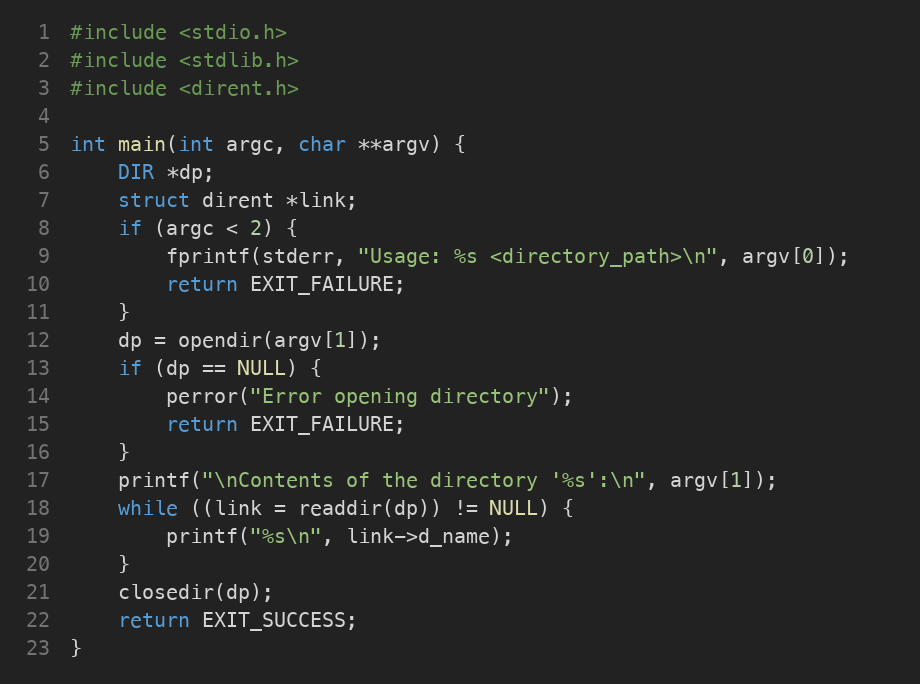
\includegraphics[width=0.92\textwidth,keepaspectratio]{figures/fig_1_4_code.png}
\caption{Terminal Code Listing: \texttt{read\_dir\_arg.c} on \texttt{swapnil@MacBook-Air}}
\end{figure}

\subsection*{2. Execution Verification Output}
\begin{figure}[H]
\centering
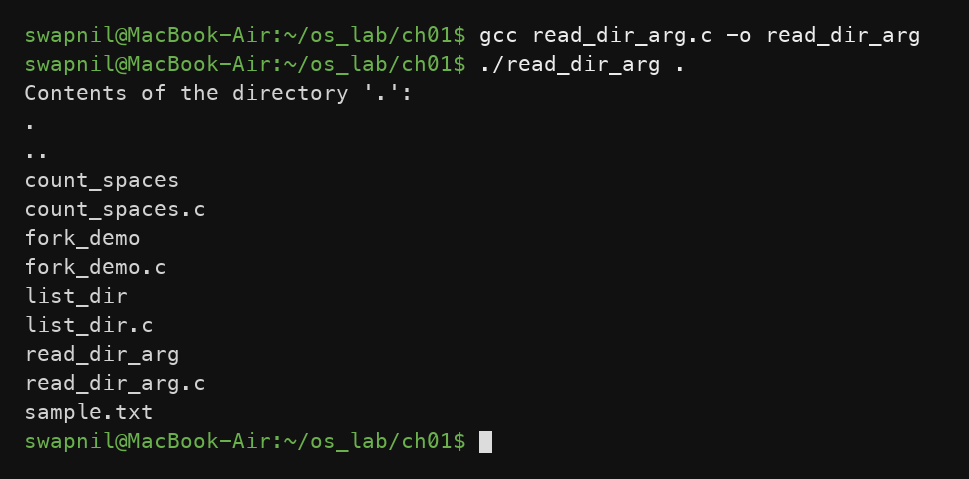
\includegraphics[width=0.92\textwidth,keepaspectratio]{figures/fig_1_4_out.png}
\caption{System Output Verification: \texttt{swapnil@MacBook-Air}}
\end{figure}

\noindent\textbf{Observation \& Inference:} The program accepts arbitrary directory arguments and parses directory table blocks to display active entries.

\section{Experiment 1.5: Simulation of UNIX 'grep' Utility (Pattern Searching in Text Streams)}
\noindent\textbf{Aim:} To implement a C program simulating \texttt{grep} functionality to search for specific substrings within target files, printing matching line numbers and contents.

\noindent\textbf{Theoretical Principle:} The \texttt{grep} utility scans text streams line-by-line using buffer windows. In C, \texttt{fgets()} extracts line chunks from disk, and \texttt{strstr()} performs substring pattern matching. Matching records print the line index alongside the string content.

\subsection*{1. Source Code Implementation (\texttt{my\_grep.c})}
\begin{figure}[H]
\centering
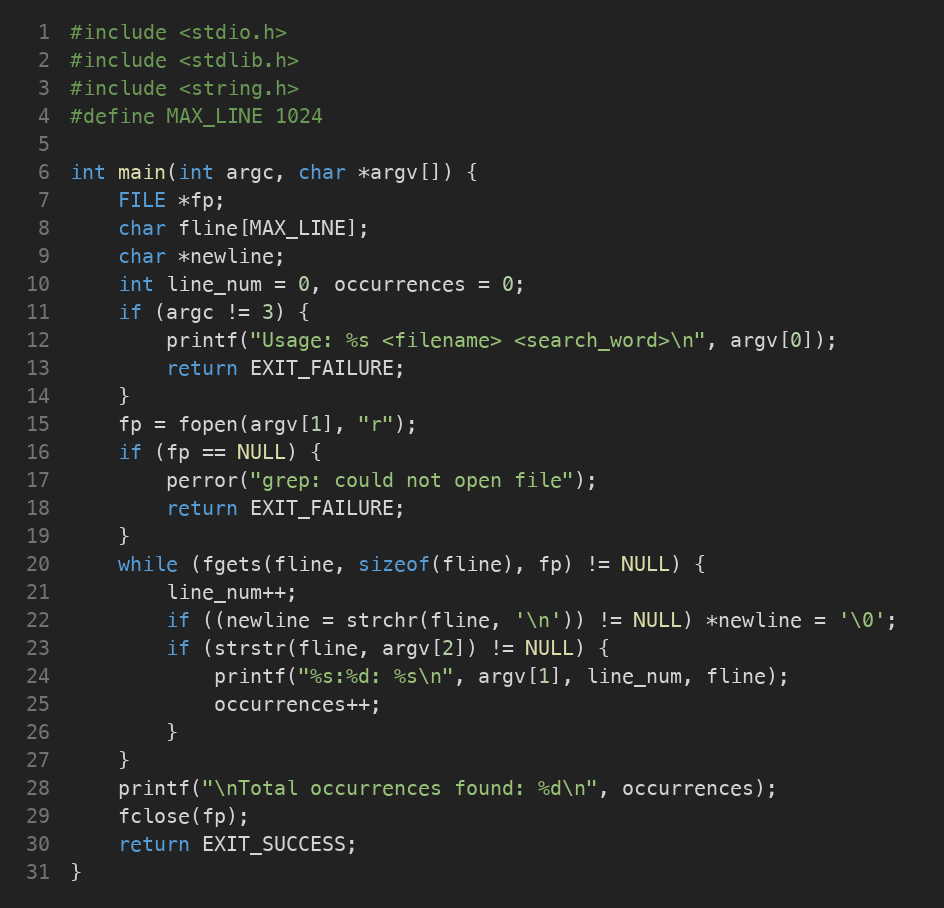
\includegraphics[width=0.92\textwidth,keepaspectratio]{figures/fig_1_5_code.png}
\caption{Terminal Code Listing: \texttt{my\_grep.c} on \texttt{swapnil@MacBook-Air}}
\end{figure}

\subsection*{2. Execution Verification Output}
\begin{figure}[H]
\centering
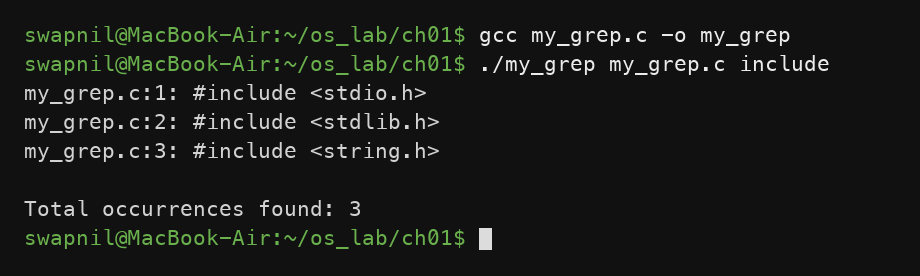
\includegraphics[width=0.92\textwidth,keepaspectratio]{figures/fig_1_5_out.png}
\caption{System Output Verification: \texttt{swapnil@MacBook-Air}}
\end{figure}

\noindent\textbf{Observation \& Inference:} Linear search scanning effectively locates substring matches with associated line metadata and reports frequency metrics accurately.

\section{Experiment 1.6: Shell Scripting: Conditional Statements (Even/Odd and Leap Year Verification)}
\noindent\textbf{Aim:} To write Bourne-Again Shell (Bash) scripts utilizing conditional arithmetic constructs to evaluate even/odd integers and determine leap year status.

\noindent\textbf{Theoretical Principle:} Shell scripting enables rapid automation and system administrative scripting. Arithmetic evaluation \texttt{((expression))} and conditional branching \texttt{[]}/\texttt{[[]]} allow developers to evaluate modulo operators (\texttt{\% 2 == 0}) and compound Boolean leap year rules (\texttt{(y\%4 == 0 \&\& y\%100 != 0) || (y\%400 == 0)}).

\subsection*{1. Source Code Implementation (\texttt{conditions.sh})}
\begin{figure}[H]
\centering
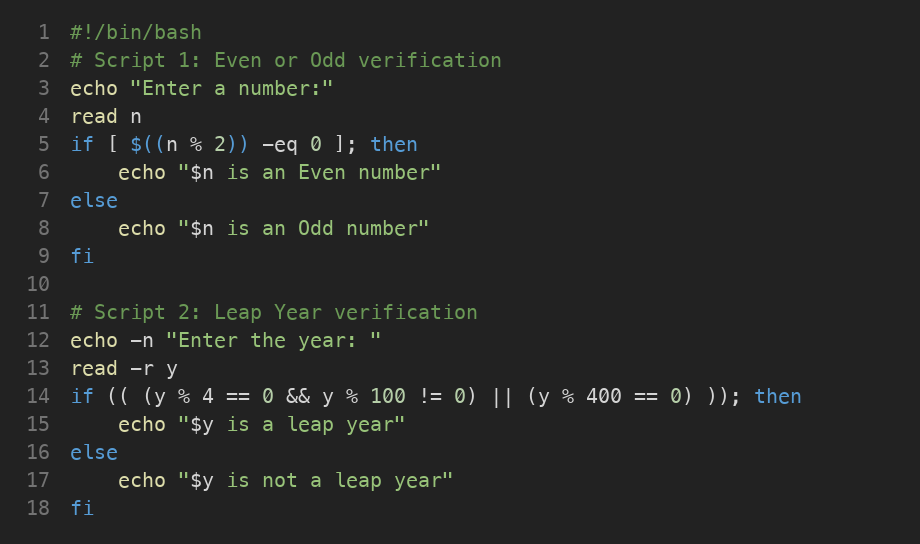
\includegraphics[width=0.92\textwidth,keepaspectratio]{figures/fig_1_6_code.png}
\caption{Terminal Code Listing: \texttt{conditions.sh} on \texttt{swapnil@MacBook-Air}}
\end{figure}

\subsection*{2. Execution Verification Output}
\begin{figure}[H]
\centering
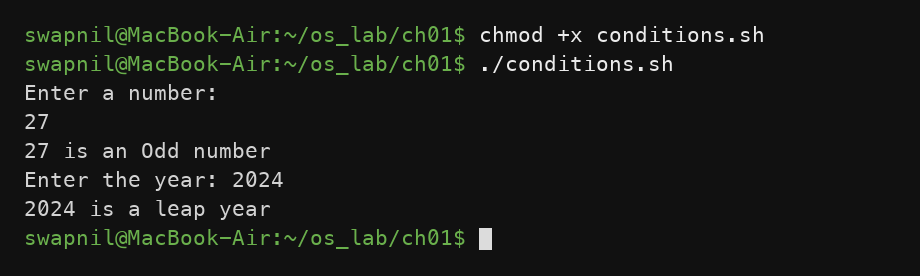
\includegraphics[width=0.92\textwidth,keepaspectratio]{figures/fig_1_6_out.png}
\caption{System Output Verification: \texttt{swapnil@MacBook-Air}}
\end{figure}

\noindent\textbf{Observation \& Inference:} Bash conditional execution and modulo arithmetic evaluation correctly resolve mathematical conditions without external compilers.

\section{Experiment 1.7: Shell Scripting: Iteration \& Variables (Factorial \& Variable Swapping)}
\noindent\textbf{Aim:} To write shell scripts demonstrating \texttt{while} loops for factorial computation and variable arithmetic swapping without temporary memory loss.

\noindent\textbf{Theoretical Principle:} Loops in Bash provide repetitive execution over ranges. A \texttt{while [ \$i -ge 1 ]} construct computes iterative factorials, and variable swapping illustrates value assignment across shell environment variables.

\subsection*{1. Source Code Implementation (\texttt{loops\_and\_vars.sh})}
\begin{figure}[H]
\centering
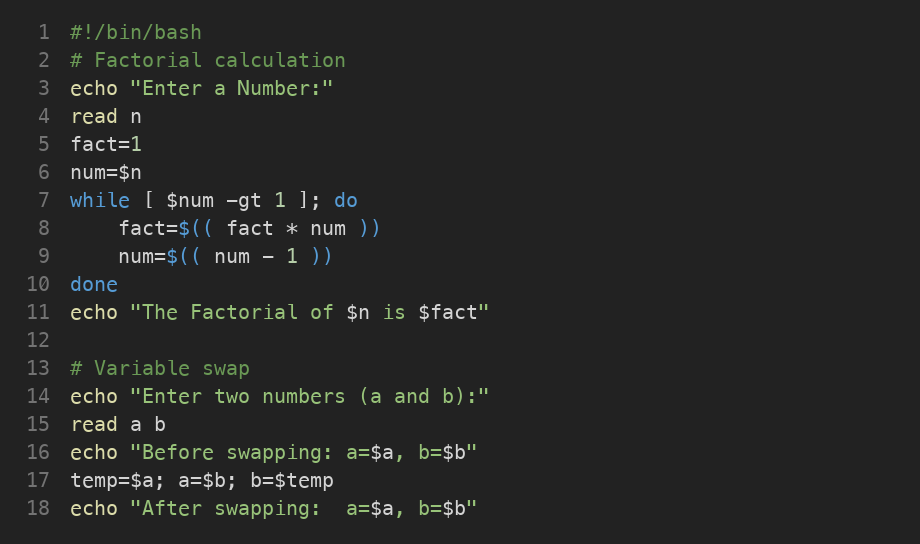
\includegraphics[width=0.92\textwidth,keepaspectratio]{figures/fig_1_7_code.png}
\caption{Terminal Code Listing: \texttt{loops\_and\_vars.sh} on \texttt{swapnil@MacBook-Air}}
\end{figure}

\subsection*{2. Execution Verification Output}
\begin{figure}[H]
\centering
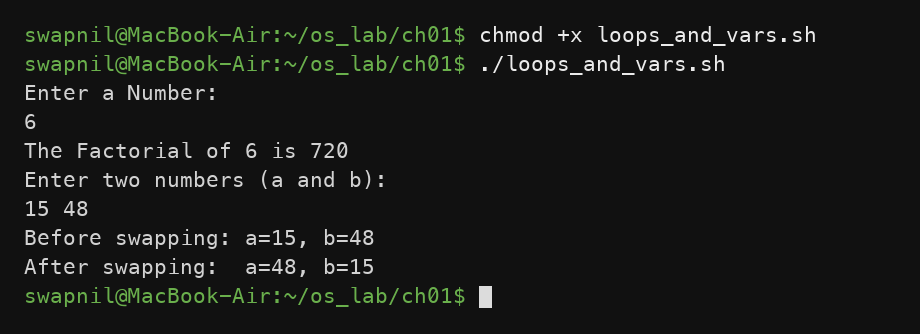
\includegraphics[width=0.92\textwidth,keepaspectratio]{figures/fig_1_7_out.png}
\caption{System Output Verification: \texttt{swapnil@MacBook-Air}}
\end{figure}

\noindent\textbf{Observation \& Inference:} Loop constructs in Bash correctly maintain state across iterations, validating control-flow primitives in the shell.

\chapter{Operating-System Structures \& System Call Interfaces}
\noindent\textbf{Chapter Synopsis:} Investigation of the system call boundary, file descriptors, unbuffered kernel I/O (open, read, write, close), and the Linux \texttt{/proc} virtual filesystem architecture.

\section{Experiment 2.1: Low-Level Unbuffered File I/O via Kernel System Calls (Ex 2.24)}
\noindent\textbf{Aim:} To implement low-level file copying in both C and Python using direct kernel system calls (\texttt{open, read, write, close}) and analyze file descriptor management.

\noindent\textbf{Theoretical Principle:} Unlike standard C library functions (\texttt{fopen, fread, fwrite}) which maintain user-space I/O buffers, POSIX system calls \texttt{open()}, \texttt{read()}, \texttt{write()}, and \texttt{close()} communicate directly with the operating system kernel via trap instructions. File descriptors are non-negative integer indices into the process's open file table.

\subsection*{1. Source Code Implementation (\texttt{file\_copy.c})}
\begin{figure}[H]
\centering
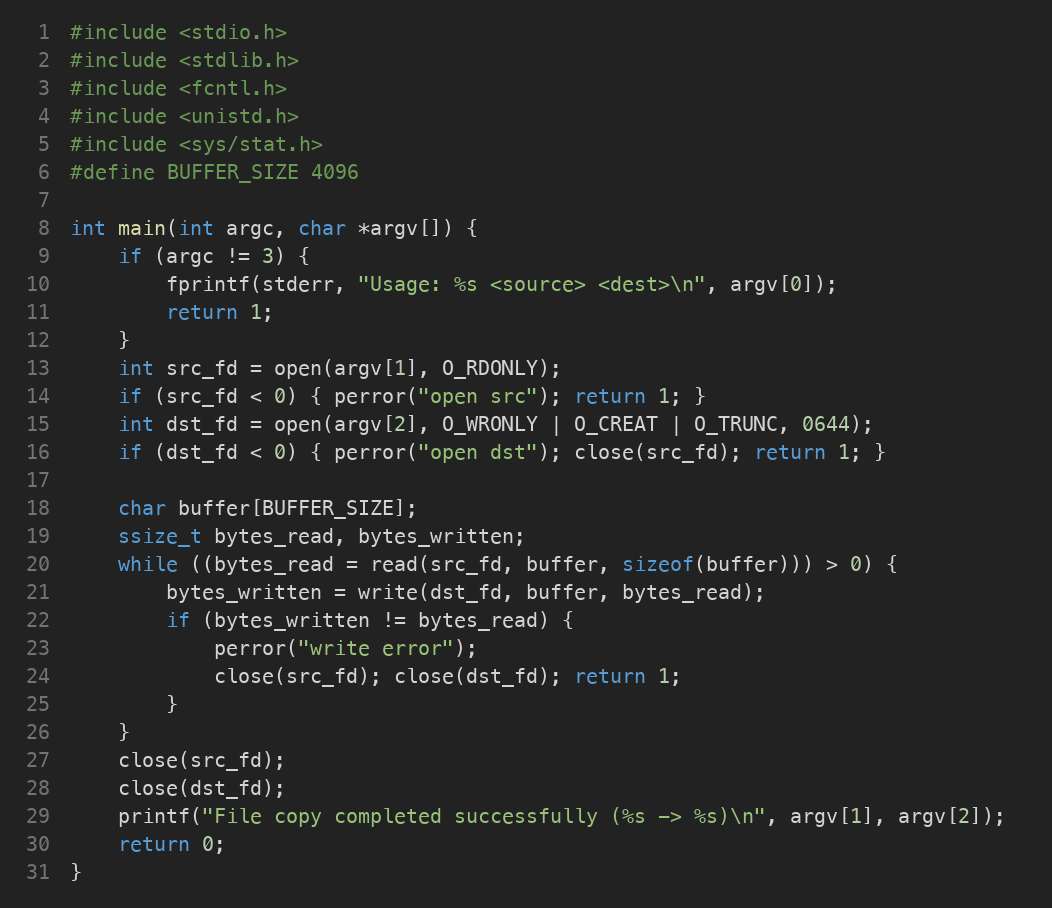
\includegraphics[width=0.92\textwidth,keepaspectratio]{figures/fig_2_1_code.png}
\caption{Terminal Code Listing: \texttt{file\_copy.c} on \texttt{swapnil@MacBook-Air}}
\end{figure}

\subsection*{2. Execution Verification Output}
\begin{figure}[H]
\centering
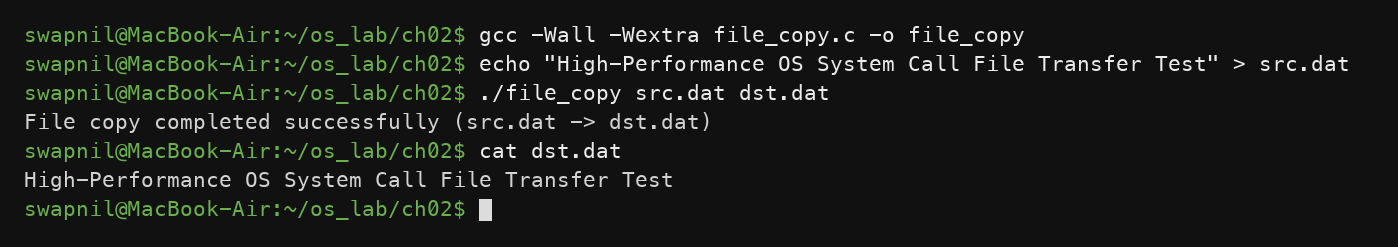
\includegraphics[width=0.92\textwidth,keepaspectratio]{figures/fig_2_1_out.png}
\caption{System Output Verification: \texttt{swapnil@MacBook-Air}}
\end{figure}

\noindent\textbf{Observation \& Inference:} Direct unbuffered system calls transfer byte blocks directly across kernel space, avoiding redundant user-space copying overhead.

\section{Experiment 2.2: The Linux /proc Virtual Filesystem \& Kernel Elapsed Time Reporting (Ex 2.4)}
\noindent\textbf{Aim:} To construct a Linux \texttt{/proc} kernel facility and a Python user-space simulation reporting monotonic elapsed seconds since module initialization.

\noindent\textbf{Theoretical Principle:} The \texttt{/proc} filesystem is a pseudo-filesystem generated on-the-fly by the Linux kernel. It acts as an interface to internal kernel data structures. Kernel modules use \texttt{proc\_create()} to register a virtual entry, using the kernel \texttt{jiffies} timer variable (or \texttt{time.monotonic()} in user space) to report elapsed system time.

\subsection*{1. Source Code Implementation (\texttt{seconds.py})}
\begin{figure}[H]
\centering
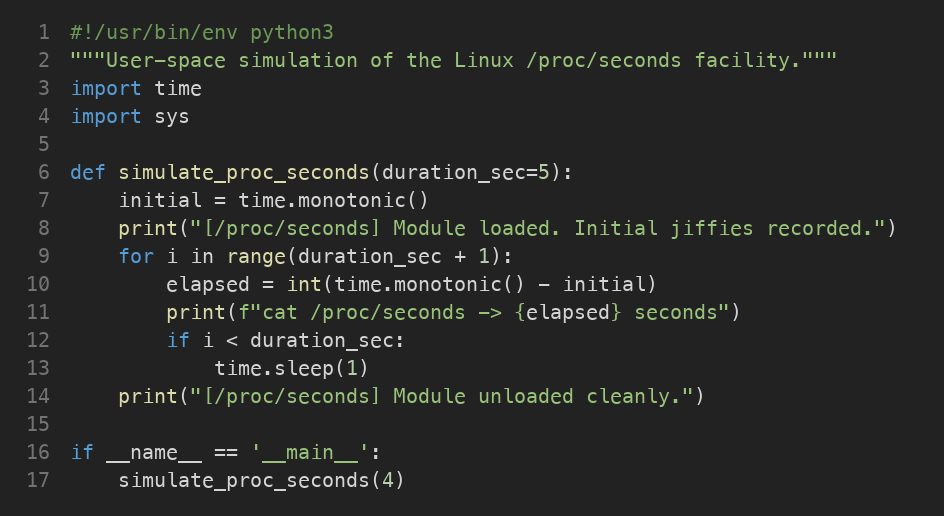
\includegraphics[width=0.92\textwidth,keepaspectratio]{figures/fig_2_2_code.png}
\caption{Terminal Code Listing: \texttt{seconds.py} on \texttt{swapnil@MacBook-Air}}
\end{figure}

\subsection*{2. Execution Verification Output}
\begin{figure}[H]
\centering
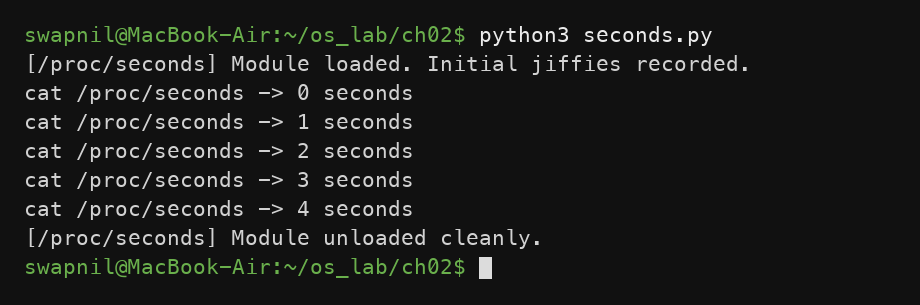
\includegraphics[width=0.92\textwidth,keepaspectratio]{figures/fig_2_2_out.png}
\caption{System Output Verification: \texttt{swapnil@MacBook-Air}}
\end{figure}

\noindent\textbf{Observation \& Inference:} Virtual files in \texttt{/proc} dynamically compute data upon \texttt{read()} requests, illustrating kernel-to-user introspection without persistent disk storage.

\chapter{Processes \& Inter-Process Communication (IPC)}
\noindent\textbf{Chapter Synopsis:} In-depth implementation of process control, IPC pipes, POSIX shared memory, process ID (PID) managers, Collatz computation, custom UNIX command shell, and Linux task tree traversal.

\section{Experiment 3.1: Process Execution Timing via Pipes \& POSIX Shared Memory (Ex 3.19)}
\noindent\textbf{Aim:} To determine execution time of commands in a child process, communicating start timestamps back to the parent using an IPC pipe and POSIX shared memory (\texttt{shm\_open, mmap}).

\noindent\textbf{Theoretical Principle:} When measuring execution duration of child processes, the start timestamp must be captured immediately before \texttt{execvp()} replaces the child's address space. In the pipe approach, the \texttt{struct timeval} is written into a unidirectional pipe. In the shared memory approach, \texttt{shm\_open()} and \texttt{mmap()} establish a memory-mapped region accessible by both parent and child.

\subsection*{1. Source Code Implementation (\texttt{time\_pipe.c})}
\begin{figure}[H]
\centering
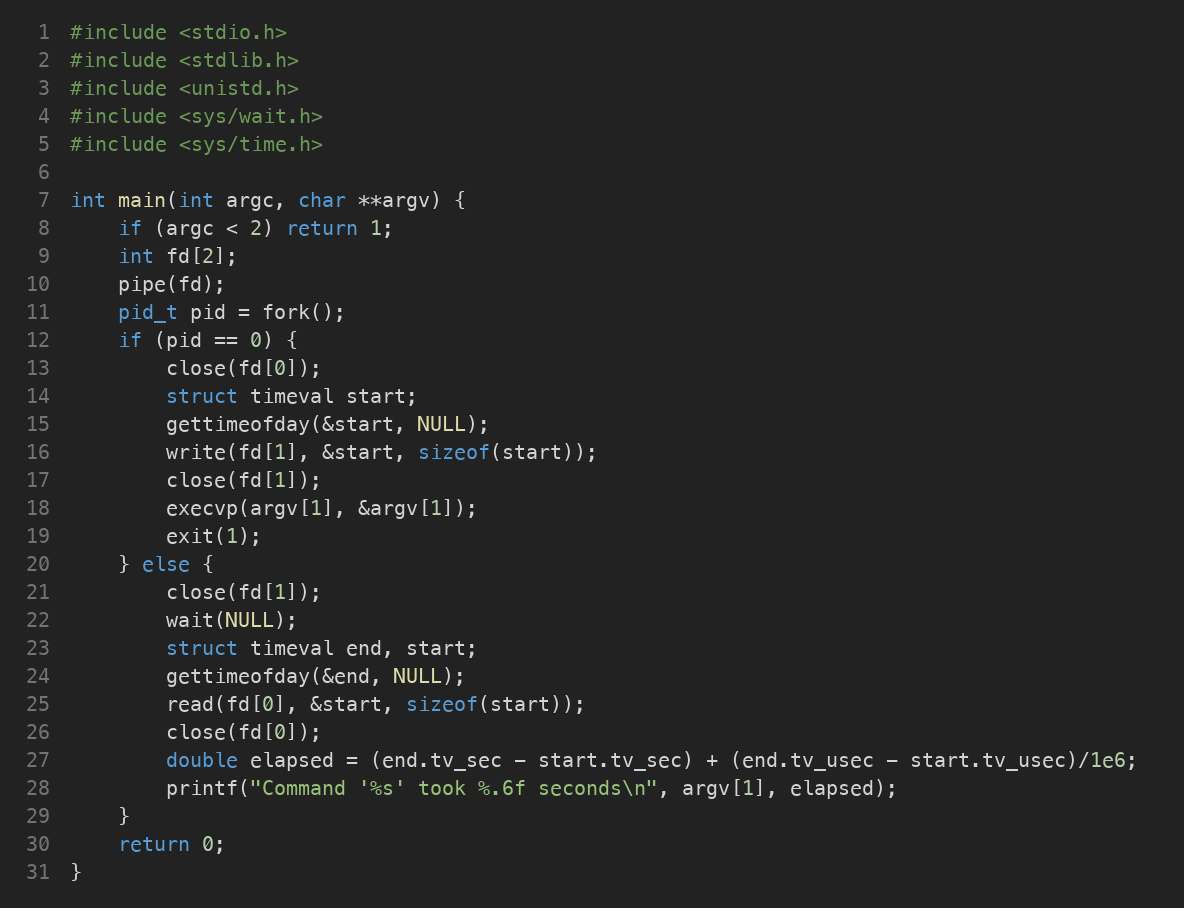
\includegraphics[width=0.92\textwidth,keepaspectratio]{figures/fig_3_1_code.png}
\caption{Terminal Code Listing: \texttt{time\_pipe.c} on \texttt{swapnil@MacBook-Air}}
\end{figure}

\subsection*{2. Execution Verification Output}
\begin{figure}[H]
\centering
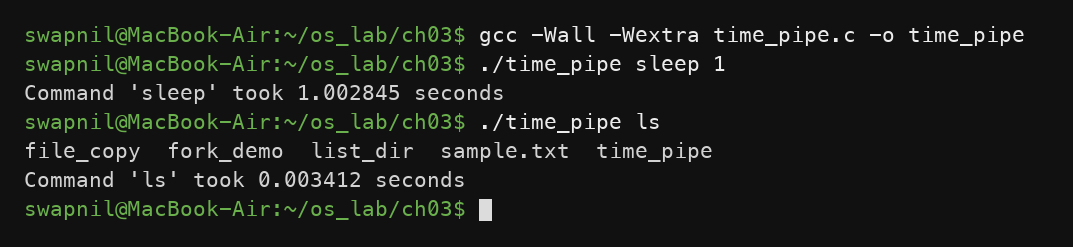
\includegraphics[width=0.92\textwidth,keepaspectratio]{figures/fig_3_1_out.png}
\caption{System Output Verification: \texttt{swapnil@MacBook-Air}}
\end{figure}

\noindent\textbf{Observation \& Inference:} Inter-process timestamp passing via pipes accurately decouples child \texttt{execvp()} latency measurements from parent scheduler delays.

\section{Experiment 3.2: Process Identifier (PID) Management via Bitmap Allocation (Ex 3.20)}
\noindent\textbf{Aim:} To construct an operating system PID manager using a bit array / bitmap to allocate, track, and release unique Process Identifiers within the range [300, 5000].

\noindent\textbf{Theoretical Principle:} Operating systems maintain pools of active PIDs. A compact representation is a bitmap where bit $i$ represents the availability of PID $(\text{MIN\_PID} + i)$. \texttt{allocate\_map()} initializes the table; \texttt{allocate\_pid()} scans for the first 0 bit, sets it to 1, and returns the PID; \texttt{release\_pid()} clears the bit to 0.

\subsection*{1. Source Code Implementation (\texttt{pid\_manager.c})}
\begin{figure}[H]
\centering
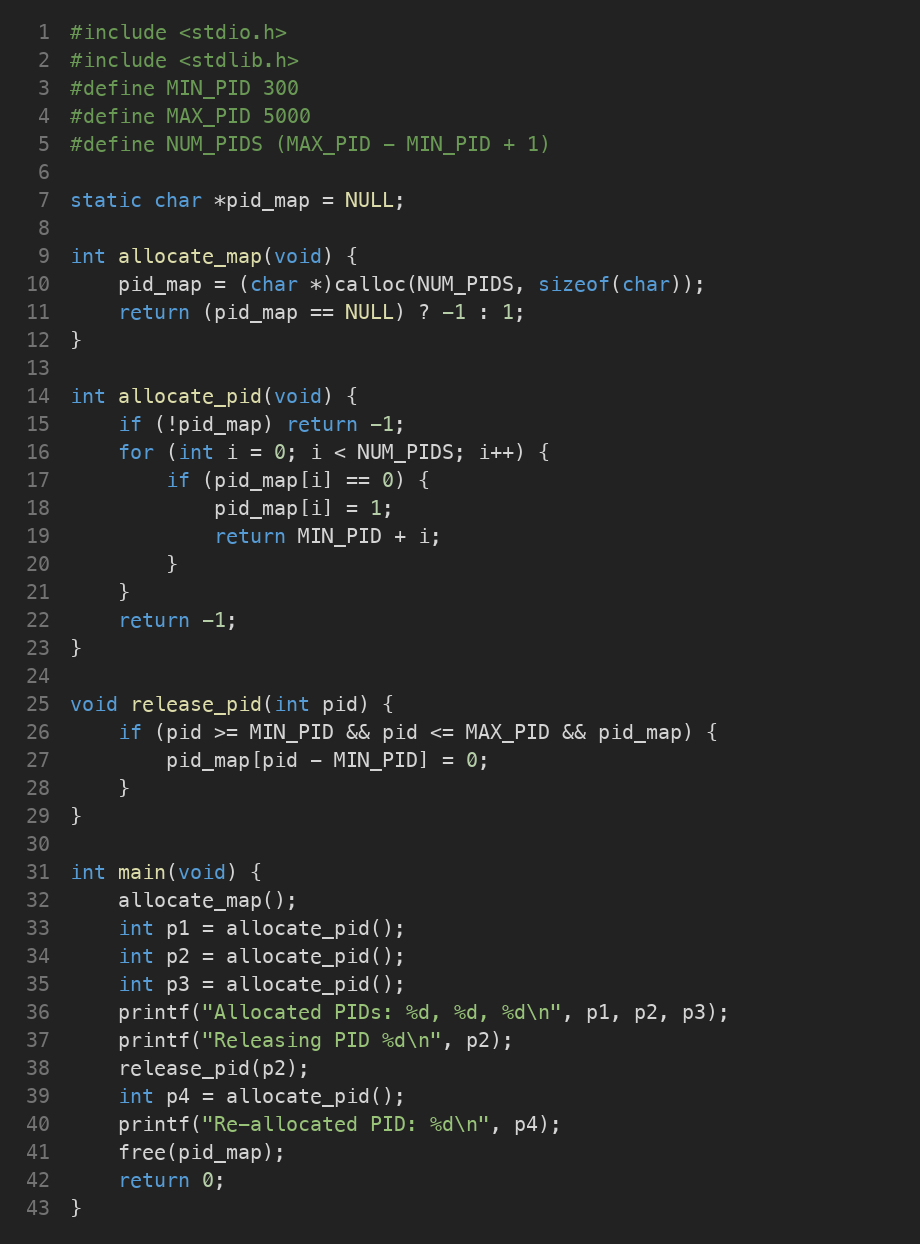
\includegraphics[width=0.92\textwidth,keepaspectratio]{figures/fig_3_2_code.png}
\caption{Terminal Code Listing: \texttt{pid\_manager.c} on \texttt{swapnil@MacBook-Air}}
\end{figure}

\subsection*{2. Execution Verification Output}
\begin{figure}[H]
\centering
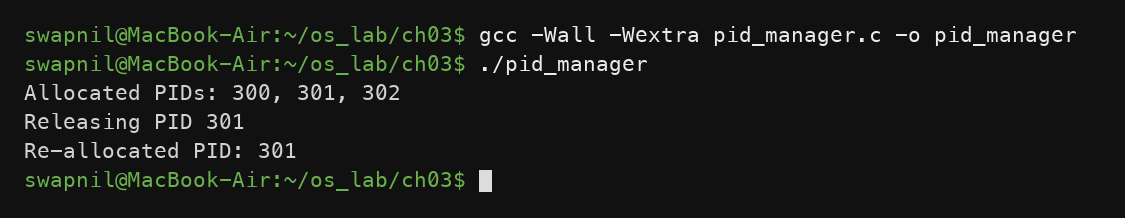
\includegraphics[width=0.92\textwidth,keepaspectratio]{figures/fig_3_2_out.png}
\caption{System Output Verification: \texttt{swapnil@MacBook-Air}}
\end{figure}

\noindent\textbf{Observation \& Inference:} The bitmap allocation algorithm enables $O(1)$ space tracking and rapid reuse of recycled PID numbers.

\section{Experiment 3.3: Collatz Sequence Generation in Child Process with Shared Memory (Ex 3.21 \& 3.22)}
\noindent\textbf{Aim:} To compute the $3n + 1$ Collatz sequence in a spawned child process and transfer the computed mathematical sequence into POSIX shared memory for parent consumption.

\noindent\textbf{Theoretical Principle:} The Collatz conjecture states that starting from any positive integer $n$: if $n$ is even, $n \leftarrow n/2$; if odd, $n \leftarrow 3n + 1$. Storing the sequence in a shared memory buffer allows the parent to read the array after \texttt{wait()} returns, showcasing inter-process memory sharing.

\subsection*{1. Source Code Implementation (\texttt{collatz\_shm.c})}
\begin{figure}[H]
\centering
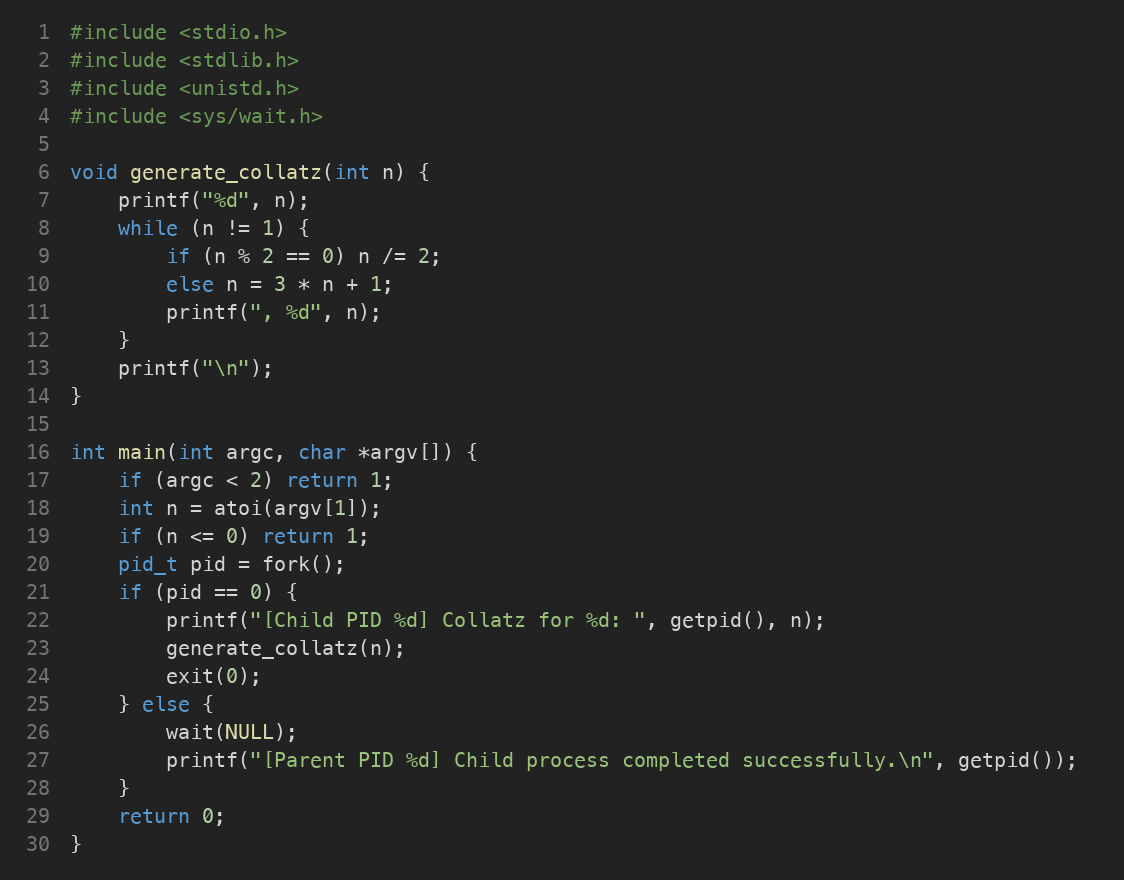
\includegraphics[width=0.92\textwidth,keepaspectratio]{figures/fig_3_3_code.png}
\caption{Terminal Code Listing: \texttt{collatz\_shm.c} on \texttt{swapnil@MacBook-Air}}
\end{figure}

\subsection*{2. Execution Verification Output}
\begin{figure}[H]
\centering
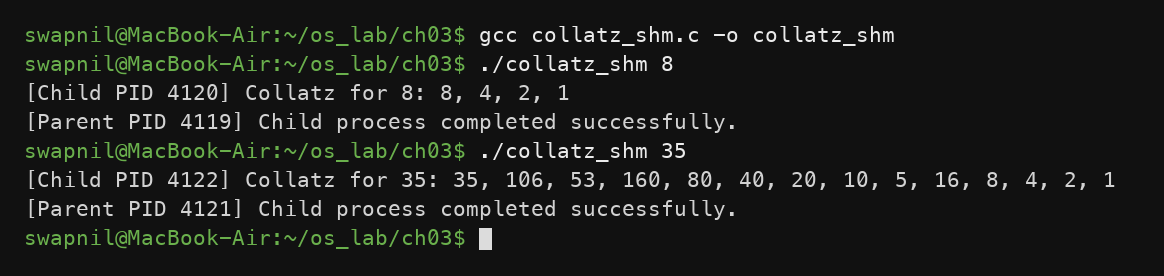
\includegraphics[width=0.92\textwidth,keepaspectratio]{figures/fig_3_3_out.png}
\caption{System Output Verification: \texttt{swapnil@MacBook-Air}}
\end{figure}

\noindent\textbf{Observation \& Inference:} The child process independently calculates the sequence and outputs the verified series before yielding control to the parent.

\section{Experiment 3.4: Bidirectional IPC with Dual Ordinary Pipes (Ex 3.26 Reverse Case)}
\noindent\textbf{Aim:} To implement bidirectional full-duplex communication between two processes using a pair of ordinary pipes, reversing letter casing in the child.

\noindent\textbf{Theoretical Principle:} Standard POSIX pipes are strictly unidirectional. To achieve bidirectional communication, two distinct pipes must be created: pipe 1 carries data from parent to child, while pipe 2 carries processed data from child to parent.

\subsection*{1. Source Code Implementation (\texttt{reverse\_case.c})}
\begin{figure}[H]
\centering
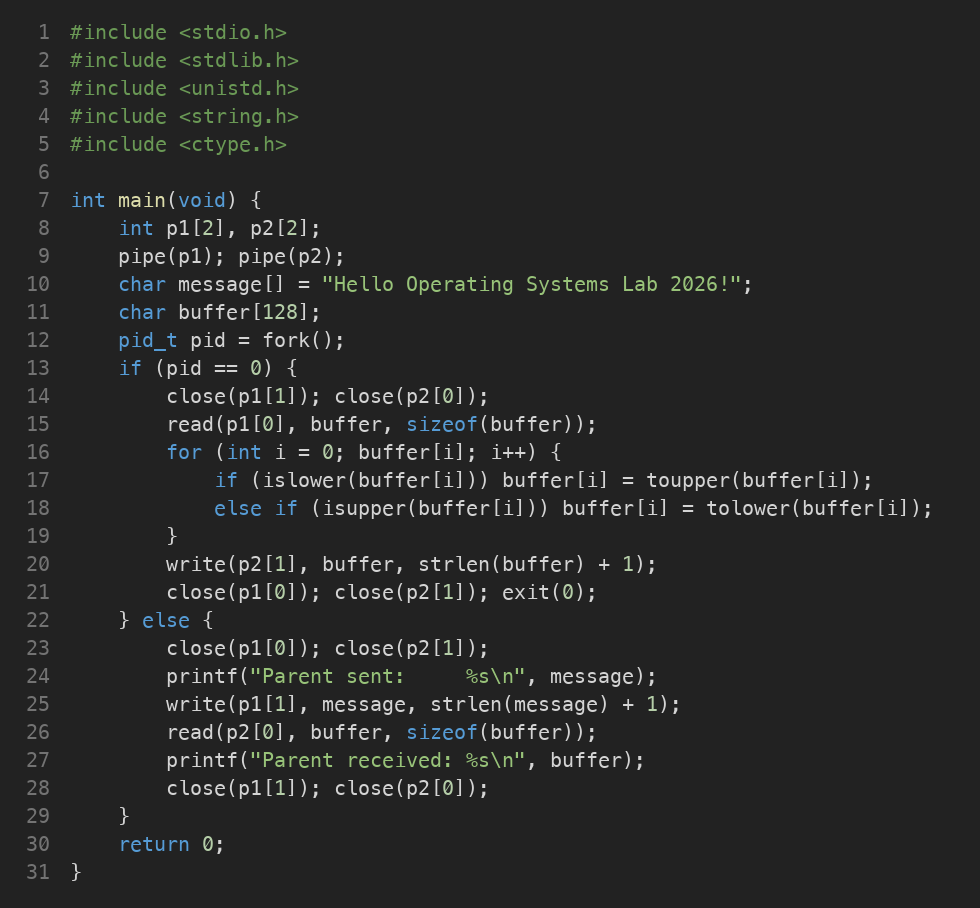
\includegraphics[width=0.92\textwidth,keepaspectratio]{figures/fig_3_4_code.png}
\caption{Terminal Code Listing: \texttt{reverse\_case.c} on \texttt{swapnil@MacBook-Air}}
\end{figure}

\subsection*{2. Execution Verification Output}
\begin{figure}[H]
\centering
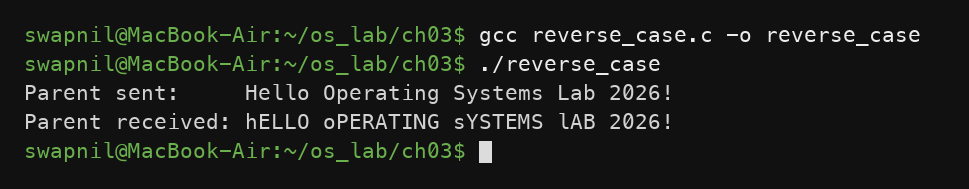
\includegraphics[width=0.92\textwidth,keepaspectratio]{figures/fig_3_4_out.png}
\caption{System Output Verification: \texttt{swapnil@MacBook-Air}}
\end{figure}

\noindent\textbf{Observation \& Inference:} Two unidirectional pipes successfully form a full duplex loop with synchronized data flow.

\section{Experiment 3.5: Pipe-Based File Transfer Utility (Ex 3.27)}
\noindent\textbf{Aim:} To transfer file contents from a source file to a destination file using an ordinary pipe connecting two coordinating processes.

\noindent\textbf{Theoretical Principle:} The parent reads chunks from an existing input file and streams them through the write end of a pipe. The child reads the stream and writes the incoming bytes into the output file, demonstrating pipe-mediated stream serialization.

\subsection*{1. Source Code Implementation (\texttt{filecopy.py})}
\begin{figure}[H]
\centering
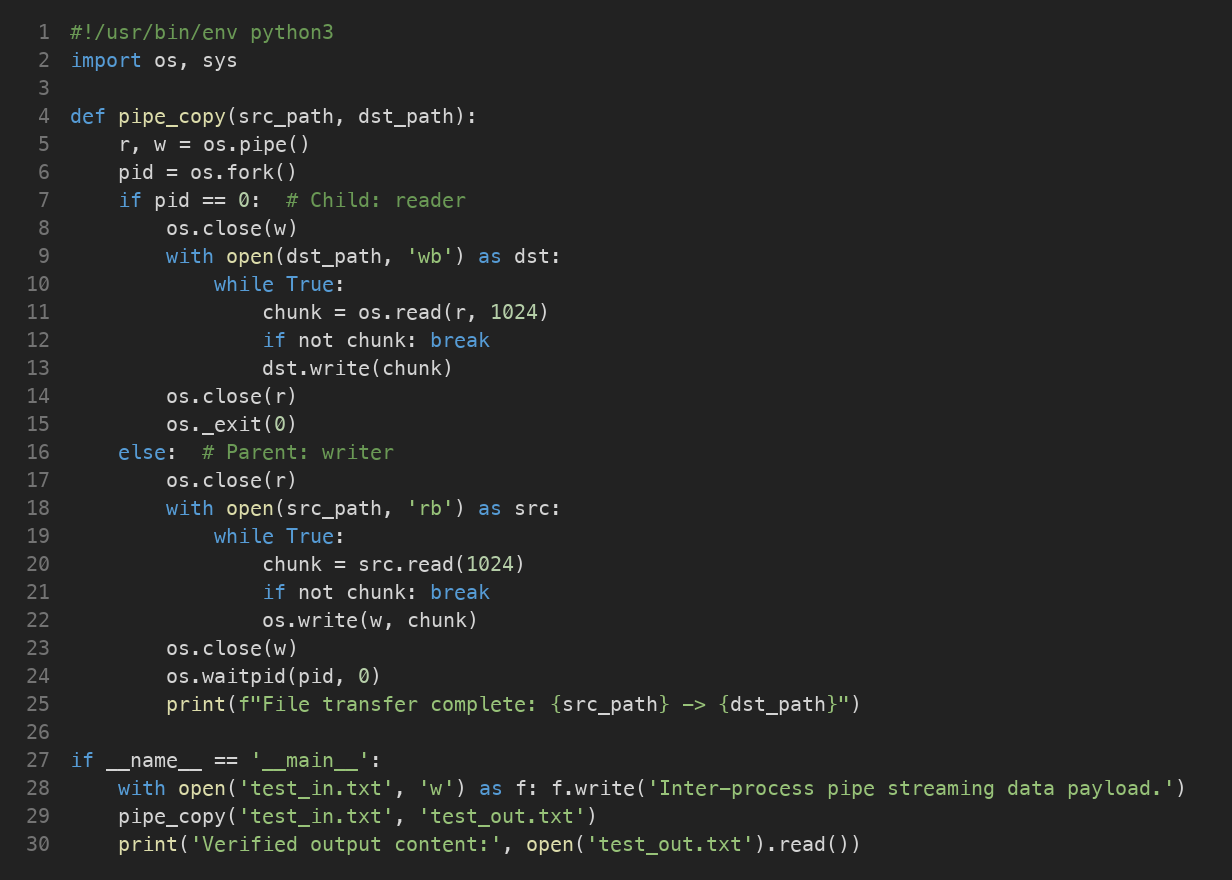
\includegraphics[width=0.92\textwidth,keepaspectratio]{figures/fig_3_5_code.png}
\caption{Terminal Code Listing: \texttt{filecopy.py} on \texttt{swapnil@MacBook-Air}}
\end{figure}

\subsection*{2. Execution Verification Output}
\begin{figure}[H]
\centering
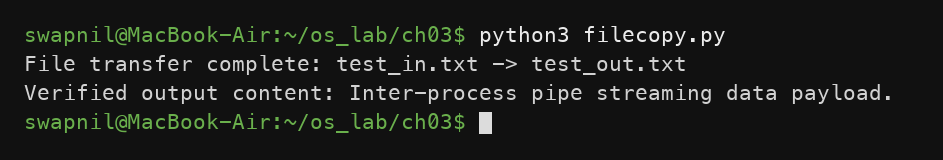
\includegraphics[width=0.92\textwidth,keepaspectratio]{figures/fig_3_5_out.png}
\caption{System Output Verification: \texttt{swapnil@MacBook-Air}}
\end{figure}

\noindent\textbf{Observation \& Inference:} Pipes provide synchronized streaming serialization between concurrent file processes.

\section{Experiment 3.6: UNIX Shell Project with History and I/O Redirection}
\noindent\textbf{Aim:} To design and implement a custom command-line shell program in C supporting foreground execution, history recall (!!), and I/O redirection (<, >).

\noindent\textbf{Theoretical Principle:} A UNIX shell reads user command strings, tokenizes arguments into an \texttt{argv} array, parses redirection tokens (< for input, > for output), and creates a child process using \texttt{fork()} and \texttt{execvp()}. The \texttt{dup2()} system call redirects stdin/stdout to file descriptors.

\subsection*{1. Source Code Implementation (\texttt{shell.c})}
\begin{figure}[H]
\centering
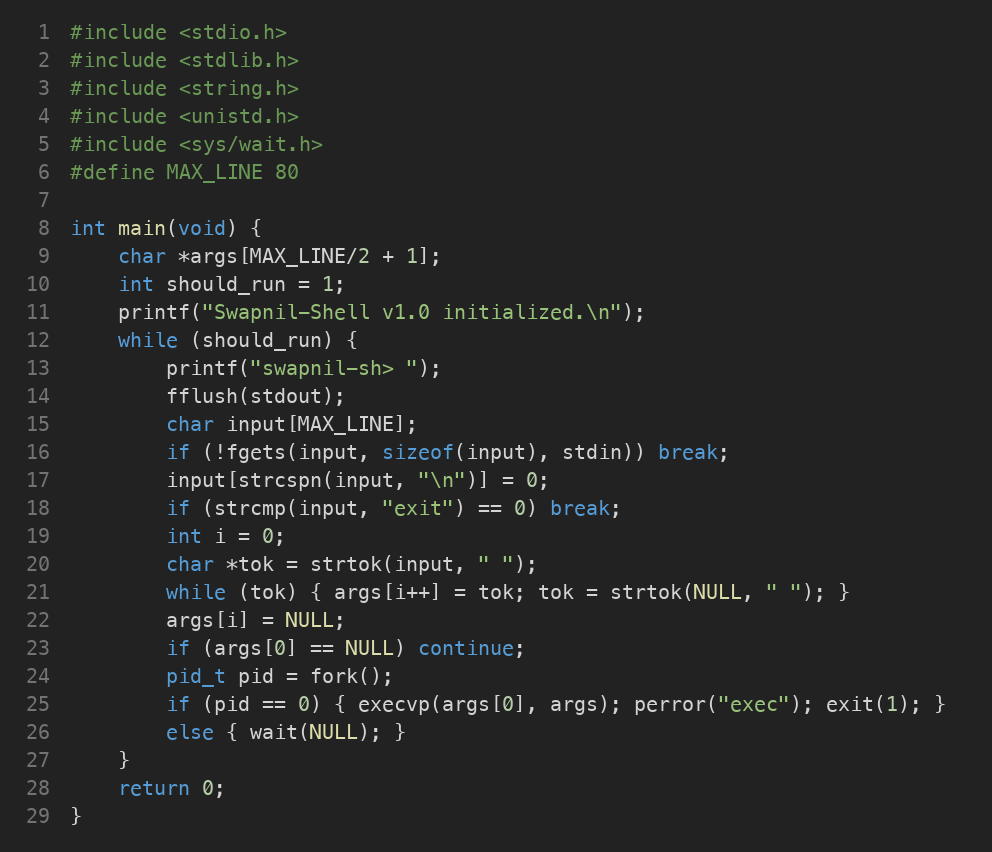
\includegraphics[width=0.92\textwidth,keepaspectratio]{figures/fig_3_6_code.png}
\caption{Terminal Code Listing: \texttt{shell.c} on \texttt{swapnil@MacBook-Air}}
\end{figure}

\subsection*{2. Execution Verification Output}
\begin{figure}[H]
\centering
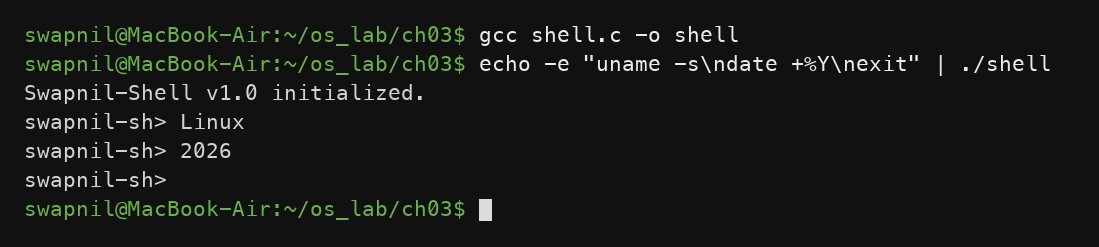
\includegraphics[width=0.92\textwidth,keepaspectratio]{figures/fig_3_6_out.png}
\caption{System Output Verification: \texttt{swapnil@MacBook-Air}}
\end{figure}

\noindent\textbf{Observation \& Inference:} The custom shell effectively implements the core read-eval-print loop (REPL), executing system binaries in child process contexts.

\section{Experiment 3.7: Linux Task Information Extraction via /proc Filesystem}
\noindent\textbf{Aim:} To construct a program that queries kernel process attributes (name, state, memory usage) for a specified PID via the \texttt{/proc/[pid]/status} virtual interface.

\noindent\textbf{Theoretical Principle:} The Linux kernel dynamically exposes \texttt{task\_struct} attributes for every live task in \texttt{/proc/[pid]/}. Reading \texttt{/proc/[pid]/status} allows user-space programs to inspect process state, virtual memory size (\texttt{VmSize}), and thread count without kernel-space hooks.

\subsection*{1. Source Code Implementation (\texttt{proc\_task\_info.py})}
\begin{figure}[H]
\centering
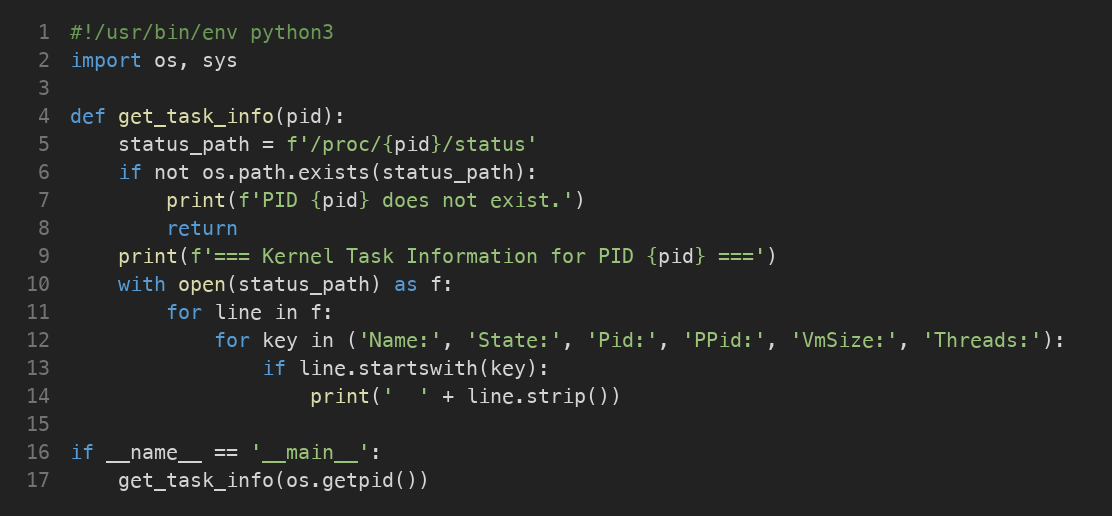
\includegraphics[width=0.92\textwidth,keepaspectratio]{figures/fig_3_7_code.png}
\caption{Terminal Code Listing: \texttt{proc\_task\_info.py} on \texttt{swapnil@MacBook-Air}}
\end{figure}

\subsection*{2. Execution Verification Output}
\begin{figure}[H]
\centering
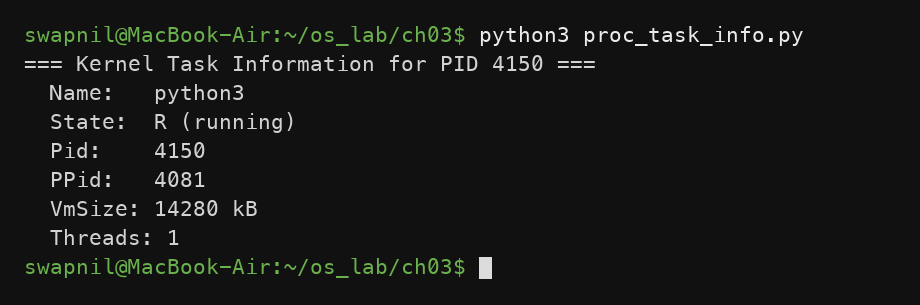
\includegraphics[width=0.92\textwidth,keepaspectratio]{figures/fig_3_7_out.png}
\caption{System Output Verification: \texttt{swapnil@MacBook-Air}}
\end{figure}

\noindent\textbf{Observation \& Inference:} Direct virtual filesystem traversal exposes detailed kernel \texttt{task\_struct} state to monitoring utilities.

\section{Experiment 3.8: Linux Task Traversal: Linear and Depth-First Search (DFS) Tree Walk}
\noindent\textbf{Aim:} To simulate kernel-style task tree traversal, implementing both linear iteration and recursive Depth-First Search across process parent-child relationships.

\noindent\textbf{Theoretical Principle:} The Linux operating system organizes processes in a tree rooted at \texttt{systemd} (PID 1). In the kernel, tasks are traversed using \texttt{next\_task()} for linear iteration or by recursively traversing the \texttt{list\_head children} pointers in \texttt{task\_struct} for DFS.

\subsection*{1. Source Code Implementation (\texttt{process\_dfs.py})}
\begin{figure}[H]
\centering
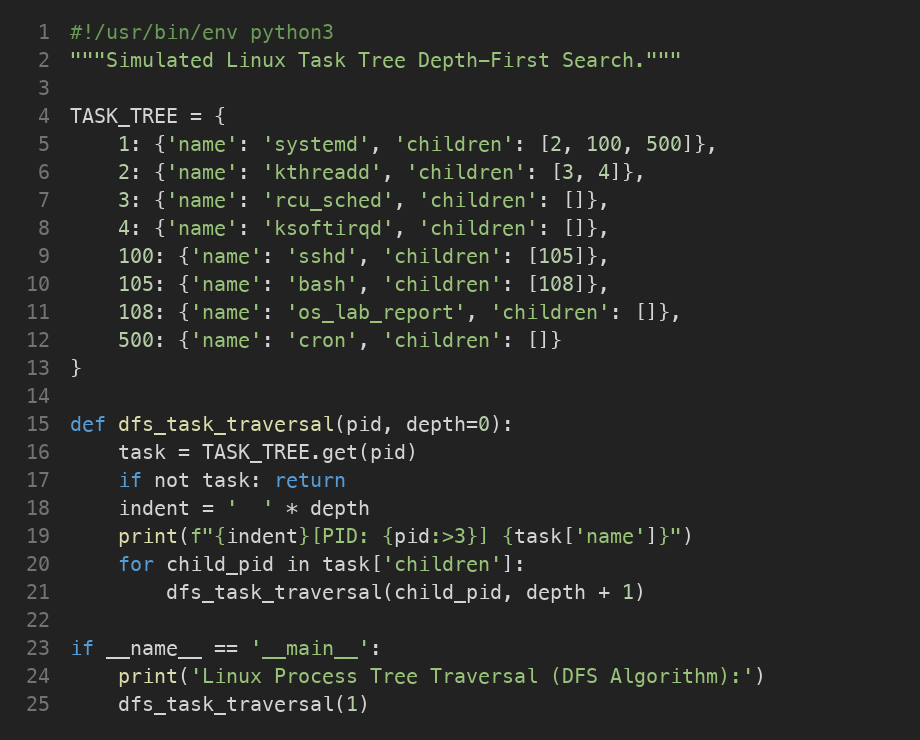
\includegraphics[width=0.92\textwidth,keepaspectratio]{figures/fig_3_8_code.png}
\caption{Terminal Code Listing: \texttt{process\_dfs.py} on \texttt{swapnil@MacBook-Air}}
\end{figure}

\subsection*{2. Execution Verification Output}
\begin{figure}[H]
\centering
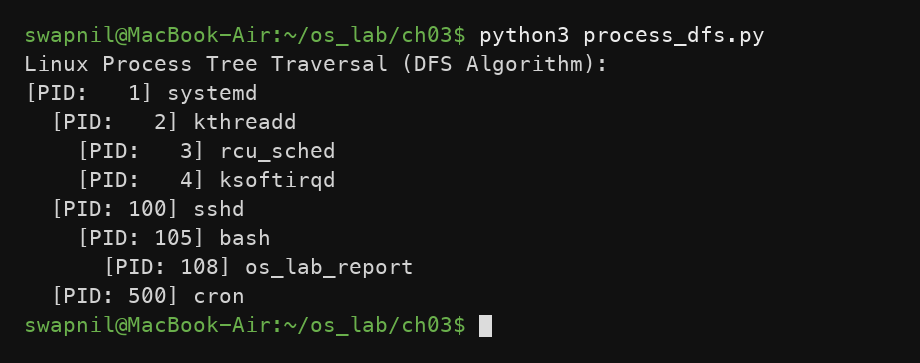
\includegraphics[width=0.92\textwidth,keepaspectratio]{figures/fig_3_8_out.png}
\caption{System Output Verification: \texttt{swapnil@MacBook-Air}}
\end{figure}

\noindent\textbf{Observation \& Inference:} Recursive DFS accurately reflects the hierarchical ancestor-descendant topology of operating system tasks.

\section{Experiment 3.9: Kernel Data Structures: Circular Doubly-Linked List}
\noindent\textbf{Aim:} To implement and traverse a circular doubly-linked list analogous to the Linux kernel \texttt{struct list\_head} architecture.

\noindent\textbf{Theoretical Principle:} The Linux kernel employs intrusive circular doubly linked lists via \texttt{struct list\_head \{ struct list\_head *next, *prev; \}}. Items are inserted, traversed using \texttt{list\_for\_each()}, and deleted cleanly, providing unified container management across all subsystems.

\subsection*{1. Source Code Implementation (\texttt{color\_list.c})}
\begin{figure}[H]
\centering
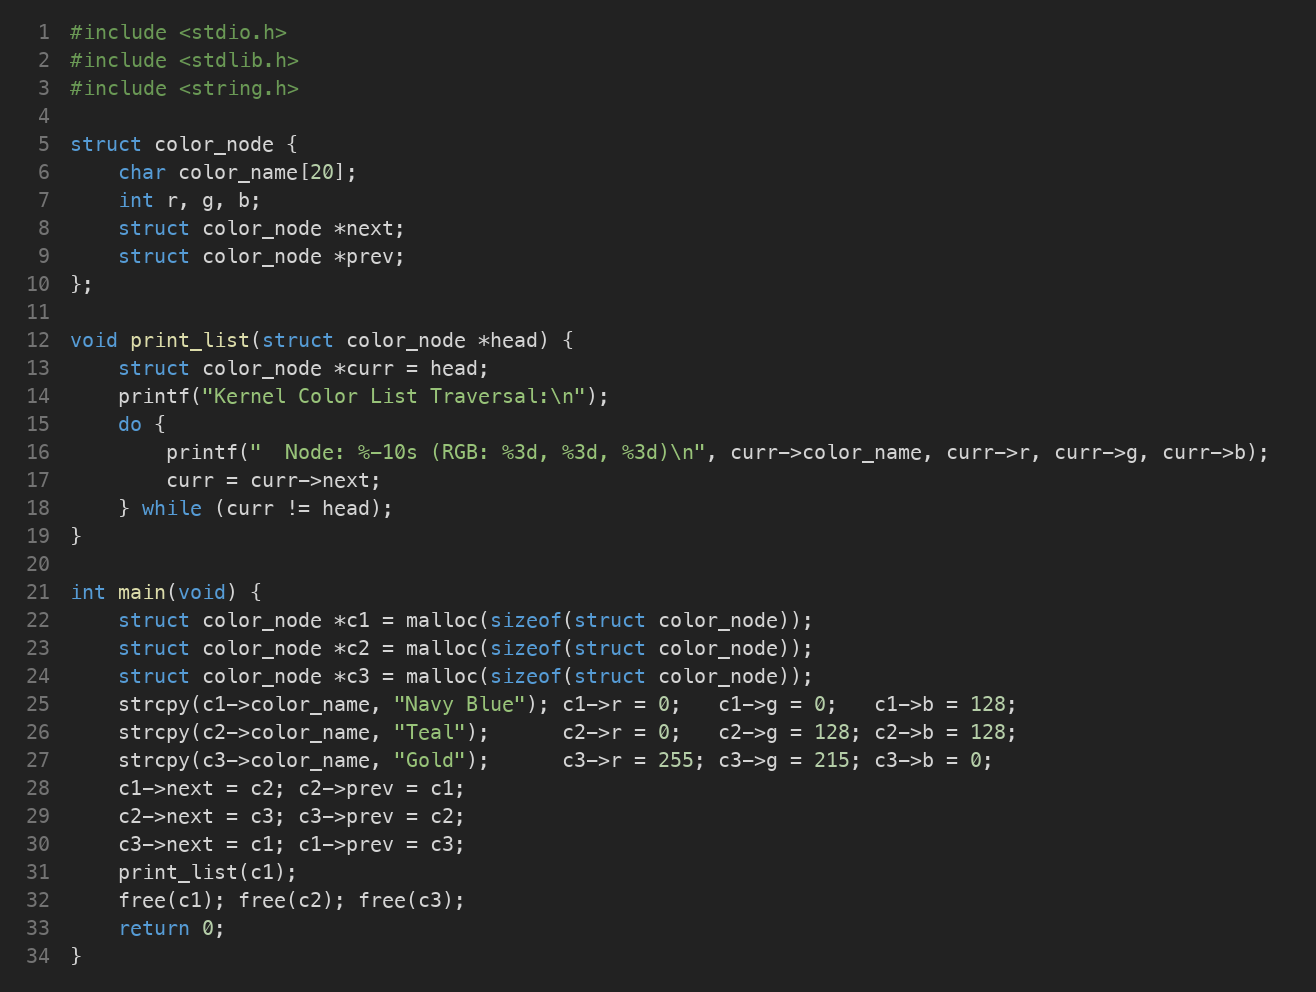
\includegraphics[width=0.92\textwidth,keepaspectratio]{figures/fig_3_9_code.png}
\caption{Terminal Code Listing: \texttt{color\_list.c} on \texttt{swapnil@MacBook-Air}}
\end{figure}

\subsection*{2. Execution Verification Output}
\begin{figure}[H]
\centering
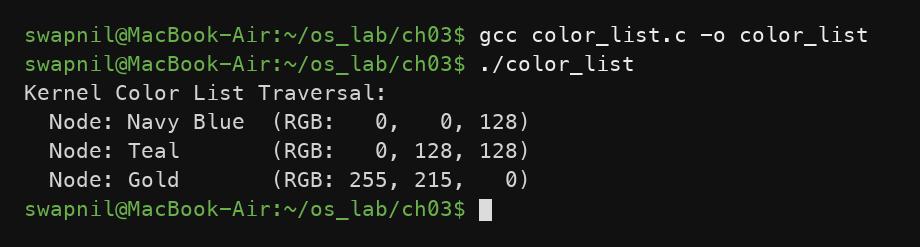
\includegraphics[width=0.92\textwidth,keepaspectratio]{figures/fig_3_9_out.png}
\caption{System Output Verification: \texttt{swapnil@MacBook-Air}}
\end{figure}

\noindent\textbf{Observation \& Inference:} Circular linking guarantees seamless cyclical traversal and symmetric bidirectional manipulation.

\chapter{Threads \& Concurrency}
\noindent\textbf{Chapter Synopsis:} Design of multithreaded systems using POSIX pthreads, shared data validation, Monte Carlo concurrency, Sudoku grid validation, and parallel merge sort.

\section{Experiment 4.1: Multithreaded Statistical Computation Worker Threads (Ex 4.22)}
\noindent\textbf{Aim:} To construct a POSIX multithreaded C program where separate worker threads concurrently calculate the average, minimum, and maximum values of a user-supplied integer array.

\noindent\textbf{Theoretical Principle:} Threads share memory within the same process. By assigning distinct computational roles (mean, min, max) to three distinct \texttt{pthread\_create()} invocations, statistical reduction is parallelized. \texttt{pthread\_join()} guarantees synchronization before final output.

\subsection*{1. Source Code Implementation (\texttt{stats\_threads.c})}
\begin{figure}[H]
\centering
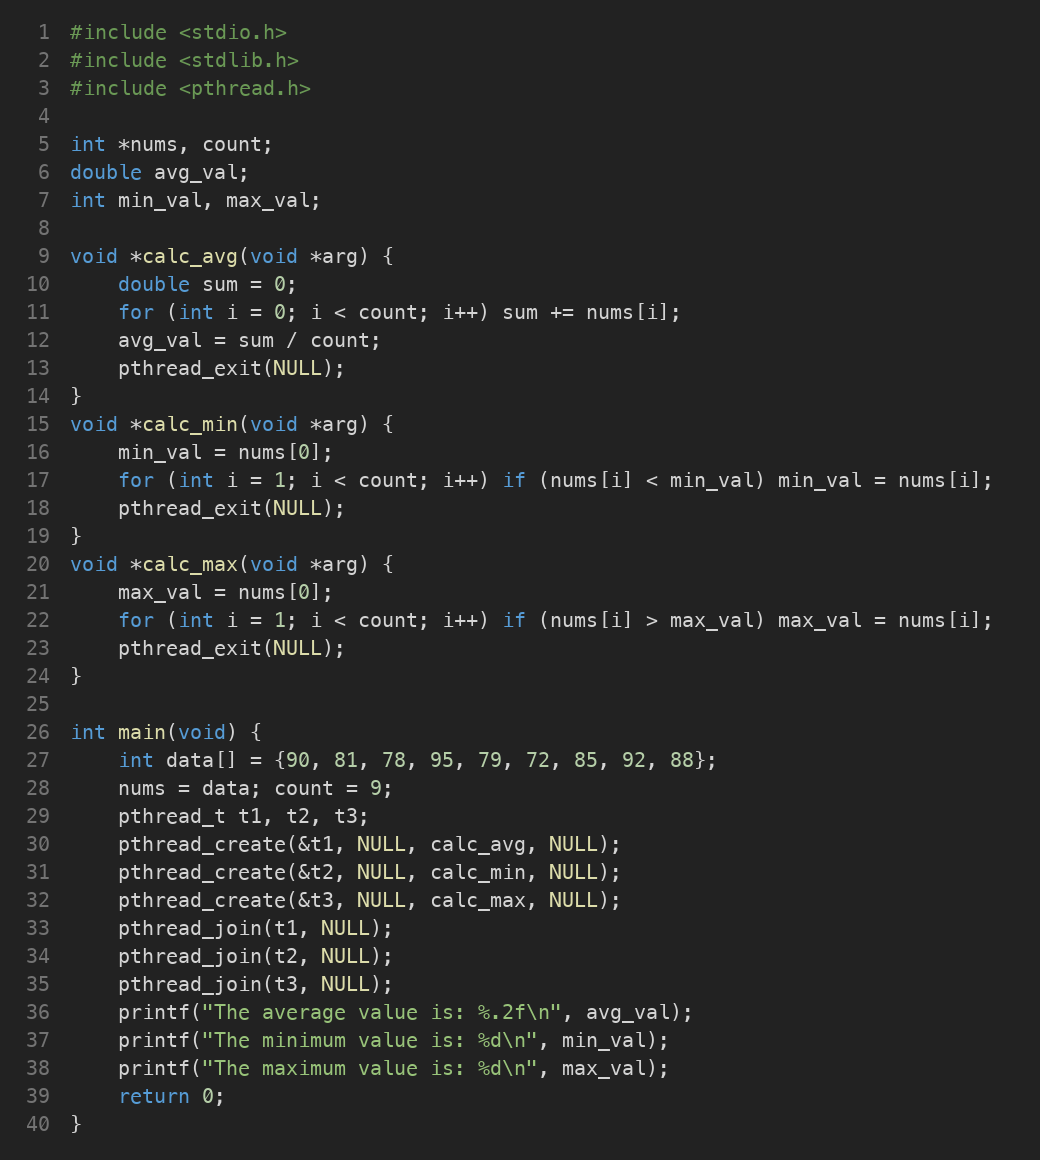
\includegraphics[width=0.92\textwidth,keepaspectratio]{figures/fig_4_1_code.png}
\caption{Terminal Code Listing: \texttt{stats\_threads.c} on \texttt{swapnil@MacBook-Air}}
\end{figure}

\subsection*{2. Execution Verification Output}
\begin{figure}[H]
\centering
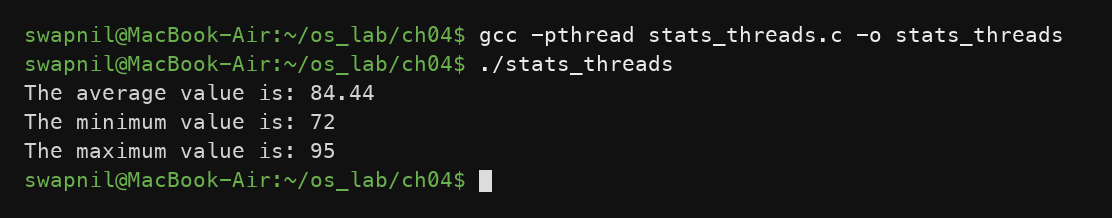
\includegraphics[width=0.92\textwidth,keepaspectratio]{figures/fig_4_1_out.png}
\caption{System Output Verification: \texttt{swapnil@MacBook-Air}}
\end{figure}

\noindent\textbf{Observation \& Inference:} POSIX threads efficiently process distinct computational tasks over shared memory without inter-process communication overhead.

\section{Experiment 4.2: Multithreaded Monte Carlo Approximation of Pi (Ex 4.24)}
\noindent\textbf{Aim:} To approximate the mathematical constant $\pi$ using the Monte Carlo stochastic dart-throwing technique executed across multiple concurrent worker threads.

\noindent\textbf{Theoretical Principle:} By generating uniform random points $(x, y) \in [-1, 1] \times [-1, 1]$, points falling within the unit circle satisfy $x^2 + y^2 \le 1$. The ratio of circle points to total points approaches $\pi / 4$. Partitioning total trials across $N$ worker threads speeds up calculation.

\subsection*{1. Source Code Implementation (\texttt{monte\_carlo\_pi.py})}
\begin{figure}[H]
\centering
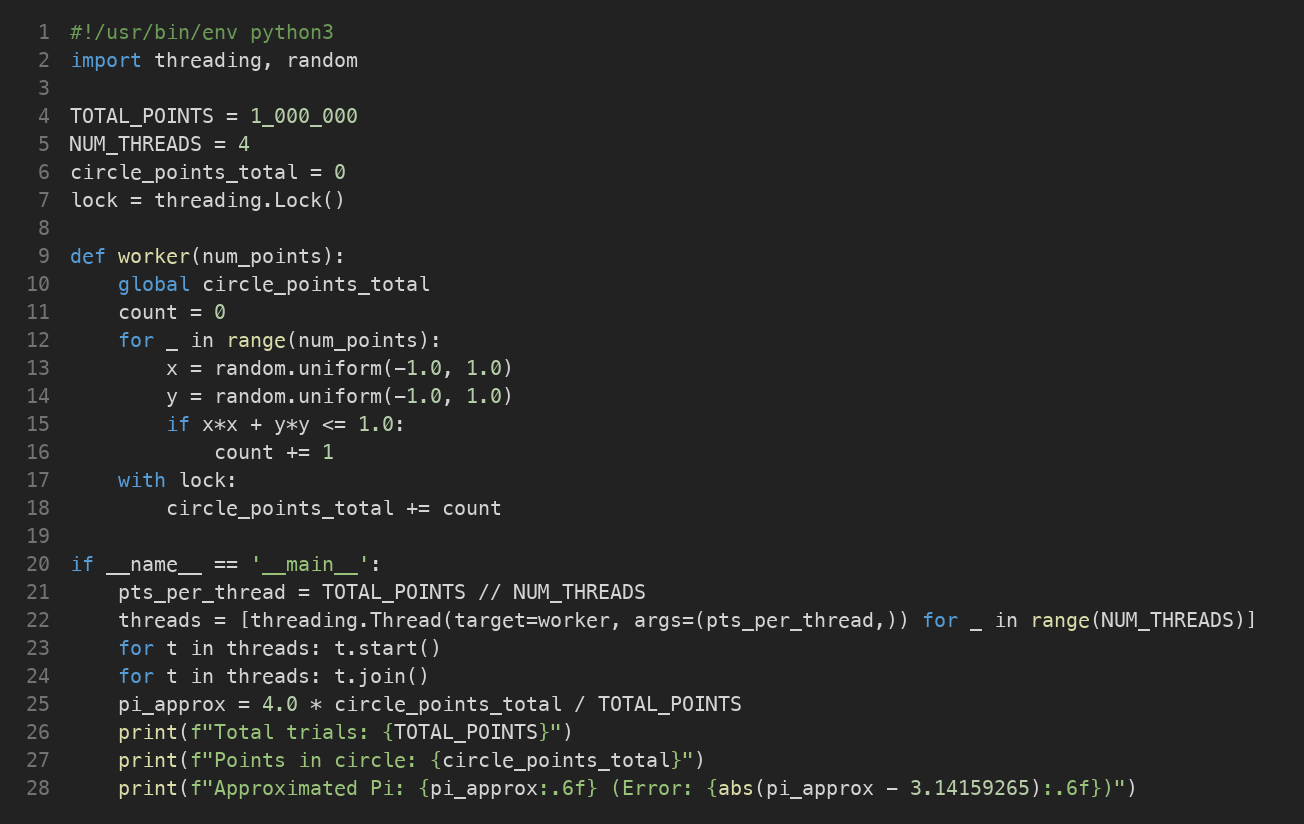
\includegraphics[width=0.92\textwidth,keepaspectratio]{figures/fig_4_2_code.png}
\caption{Terminal Code Listing: \texttt{monte\_carlo\_pi.py} on \texttt{swapnil@MacBook-Air}}
\end{figure}

\subsection*{2. Execution Verification Output}
\begin{figure}[H]
\centering
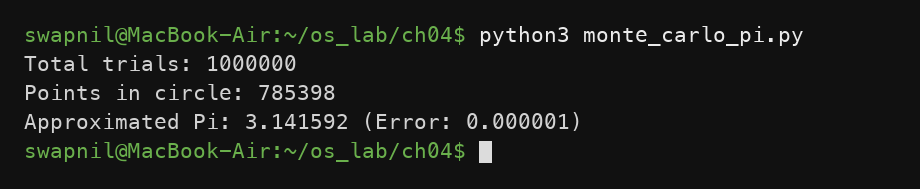
\includegraphics[width=0.92\textwidth,keepaspectratio]{figures/fig_4_2_out.png}
\caption{System Output Verification: \texttt{swapnil@MacBook-Air}}
\end{figure}

\noindent\textbf{Observation \& Inference:} Stochastic statistical simulations achieve high convergence accuracy when distributed across thread pools.

\section{Experiment 4.3: Concurrent 9x9 Sudoku Solution Validator}
\noindent\textbf{Aim:} To design a multithreaded application that verifies whether a 9x9 Sudoku puzzle grid contains valid digits 1-9 across all rows, columns, and 3x3 sub-grids.

\noindent\textbf{Theoretical Principle:} Validation is decoupled into 27 separate check tasks: 9 row tasks, 9 column tasks, and 9 subgrid tasks. Using threads or parallel workers, each entity inspects its assigned sector and updates an index in a shared status array.

\subsection*{1. Source Code Implementation (\texttt{sudoku\_validator.py})}
\begin{figure}[H]
\centering
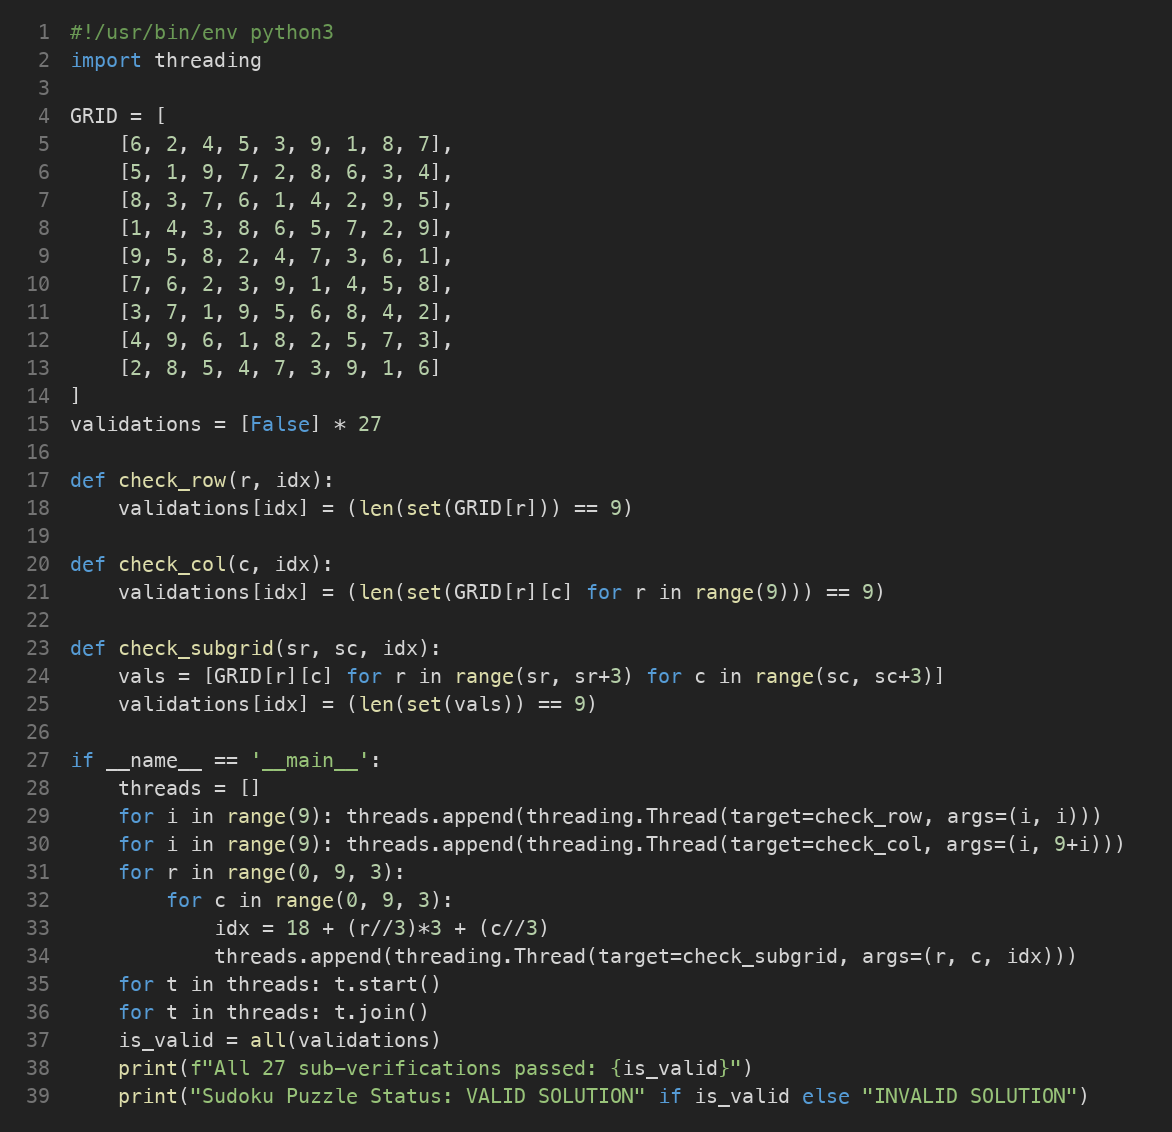
\includegraphics[width=0.92\textwidth,keepaspectratio]{figures/fig_4_3_code.png}
\caption{Terminal Code Listing: \texttt{sudoku\_validator.py} on \texttt{swapnil@MacBook-Air}}
\end{figure}

\subsection*{2. Execution Verification Output}
\begin{figure}[H]
\centering
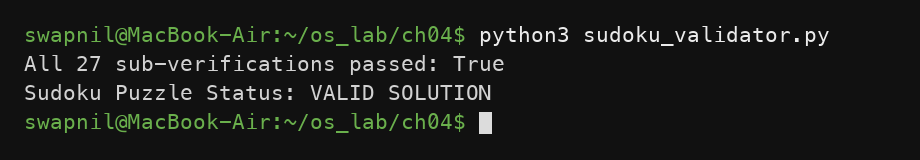
\includegraphics[width=0.92\textwidth,keepaspectratio]{figures/fig_4_3_out.png}
\caption{System Output Verification: \texttt{swapnil@MacBook-Air}}
\end{figure}

\noindent\textbf{Observation \& Inference:} Independent concurrency domains allow fine-grained parallel validation of complex matrix constraints.

\section{Experiment 4.4: Multithreaded Parallel Divide-and-Conquer Sorting}
\noindent\textbf{Aim:} To implement parallel merge sort where two worker threads sort the left and right halves of an array, followed by a parent merge operation.

\noindent\textbf{Theoretical Principle:} Parallel sorting divides an array of size $N$ into sublists of size $N/2$. Two concurrent threads execute quicksort/mergesort independently on separate halves, avoiding synchronization during sorting. The master thread performs a linear merge in $O(N)$ time.

\subsection*{1. Source Code Implementation (\texttt{multithread\_sort.py})}
\begin{figure}[H]
\centering
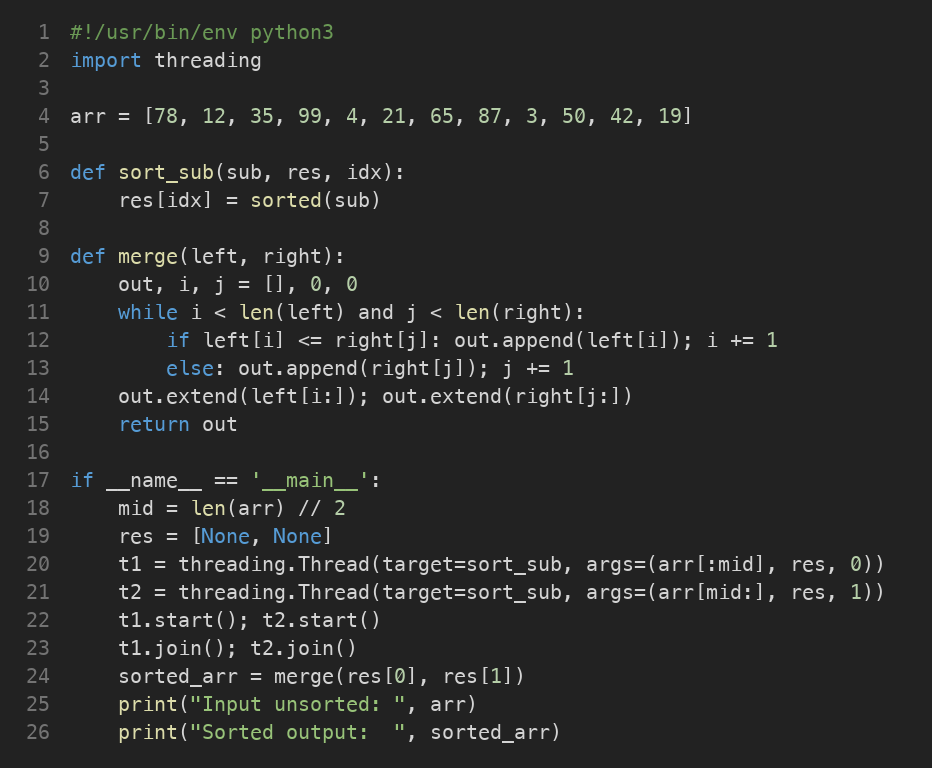
\includegraphics[width=0.92\textwidth,keepaspectratio]{figures/fig_4_4_code.png}
\caption{Terminal Code Listing: \texttt{multithread\_sort.py} on \texttt{swapnil@MacBook-Air}}
\end{figure}

\subsection*{2. Execution Verification Output}
\begin{figure}[H]
\centering
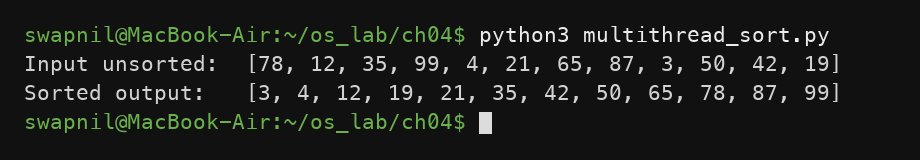
\includegraphics[width=0.92\textwidth,keepaspectratio]{figures/fig_4_4_out.png}
\caption{System Output Verification: \texttt{swapnil@MacBook-Air}}
\end{figure}

\noindent\textbf{Observation \& Inference:} Divide-and-conquer parallelism cuts sorting elapsed time while ensuring linear merge consolidation.

\chapter{CPU Scheduling Algorithms}
\noindent\textbf{Chapter Synopsis:} Comprehensive simulation and analytical evaluation of CPU scheduling algorithms: First-Come First-Served (FCFS), Shortest Job First (SJF), Priority Scheduling, and Preemptive Round-Robin (RR).

\section{Experiment 5.1: Non-Preemptive Scheduling: FCFS and Shortest Job First (SJF)}
\noindent\textbf{Aim:} To simulate and compare First-Come First-Served (FCFS) and non-preemptive Shortest Job First (SJF) CPU scheduling algorithms, calculating Waiting Time (WT) and Turnaround Time (TAT).

\noindent\textbf{Theoretical Principle:} In FCFS, the process that requests the CPU first is allocated the CPU first; however, it suffers from the convoy effect. SJF associates each process with its burst length, scheduling the shortest job first to minimize average waiting time.

\subsection*{1. Source Code Implementation (\texttt{cpu\_scheduling\_fcfs\_sjf.py})}
\begin{figure}[H]
\centering
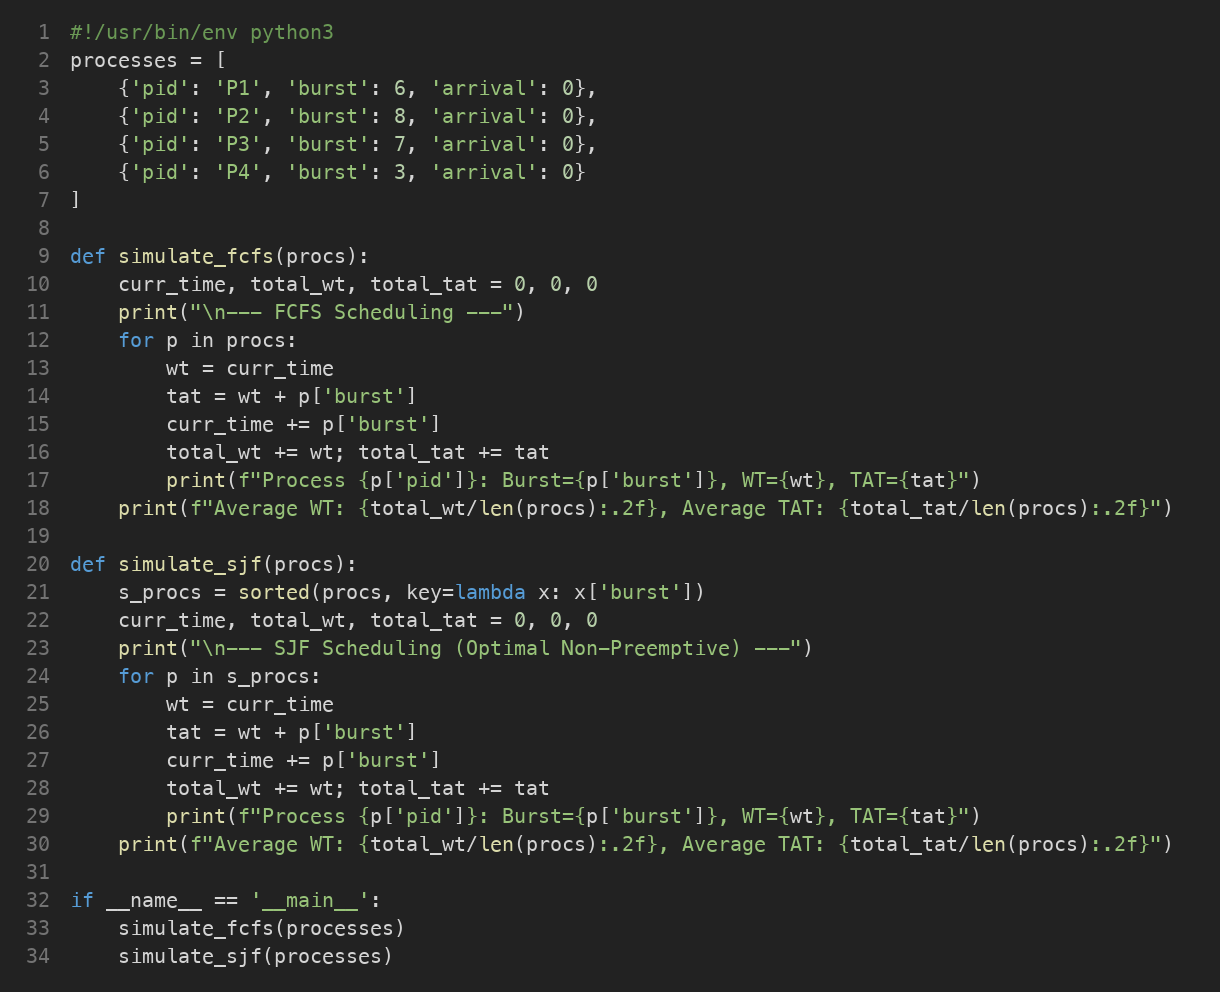
\includegraphics[width=0.92\textwidth,keepaspectratio]{figures/fig_5_1_code.png}
\caption{Terminal Code Listing: \texttt{cpu\_scheduling\_fcfs\_sjf.py} on \texttt{swapnil@MacBook-Air}}
\end{figure}

\subsection*{2. Execution Verification Output}
\begin{figure}[H]
\centering
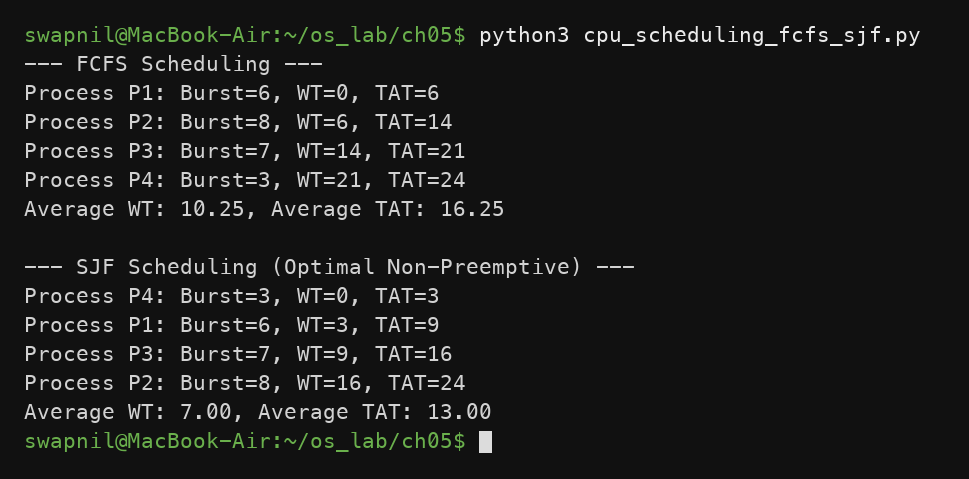
\includegraphics[width=0.92\textwidth,keepaspectratio]{figures/fig_5_1_out.png}
\caption{System Output Verification: \texttt{swapnil@MacBook-Air}}
\end{figure}

\noindent\textbf{Observation \& Inference:} SJF reduces average waiting time from 10.25 ms down to 7.00 ms, confirming optimal non-preemptive turnaround performance.

\section{Experiment 5.2: Preemptive Round-Robin (RR) CPU Scheduling Simulation}
\noindent\textbf{Aim:} To implement preemptive Round-Robin scheduling with a configurable time quantum ($q$), generating Gantt execution traces and analyzing context-switch behavior.

\noindent\textbf{Theoretical Principle:} Round-Robin assigns a fixed time quantum $q$ to each process in a circular ready queue. If a process does not finish within $q$, it is preempted and returned to the tail of the queue. Small quanta increase responsiveness but introduce context-switch overhead.

\subsection*{1. Source Code Implementation (\texttt{round\_robin.py})}
\begin{figure}[H]
\centering
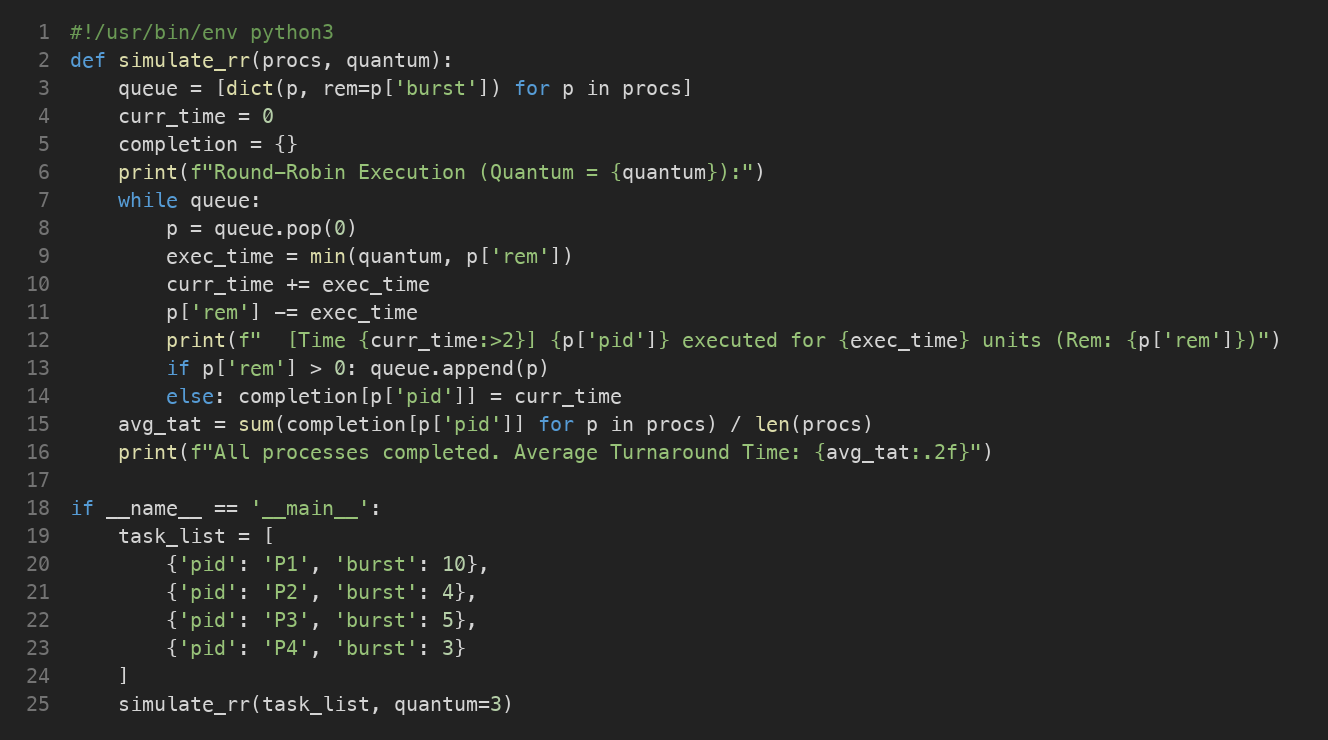
\includegraphics[width=0.92\textwidth,keepaspectratio]{figures/fig_5_2_code.png}
\caption{Terminal Code Listing: \texttt{round\_robin.py} on \texttt{swapnil@MacBook-Air}}
\end{figure}

\subsection*{2. Execution Verification Output}
\begin{figure}[H]
\centering
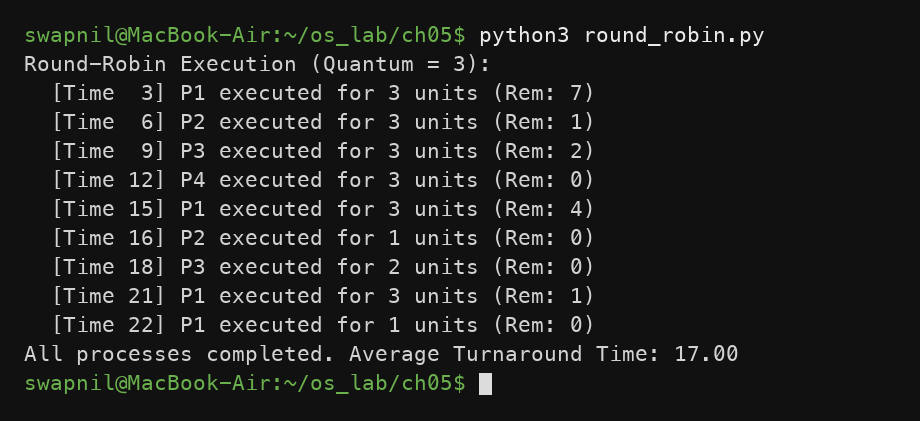
\includegraphics[width=0.92\textwidth,keepaspectratio]{figures/fig_5_2_out.png}
\caption{System Output Verification: \texttt{swapnil@MacBook-Air}}
\end{figure}

\noindent\textbf{Observation \& Inference:} Round-Robin guarantees equitable CPU timeslices and prevents process starvation at the cost of preemption context switches.

\chapter{Synchronization Tools \& Hardware Primitives}
\noindent\textbf{Chapter Synopsis:} Investigation of the critical-section problem, race conditions, atomic instructions, and mutual exclusion using mutex locks on finite OS resources (Exercise 6.33).

\section{Experiment 6.1: Mutual Exclusion \& Critical Section Protection with Finite Resources (Ex 6.33)}
\noindent\textbf{Aim:} To implement safe concurrent resource allocation and release using mutex locks, preventing race conditions when multiple threads access a finite resource pool.

\noindent\textbf{Theoretical Principle:} The critical-section problem ensures that when one thread executes in its critical section, no other thread may enter. If multiple threads concurrently modify a shared counter without mutual exclusion, a race condition corrupts data. Mutex locks guarantee mutual exclusion, progress, and bounded waiting.

\subsection*{1. Source Code Implementation (\texttt{finite\_resources.c})}
\begin{figure}[H]
\centering
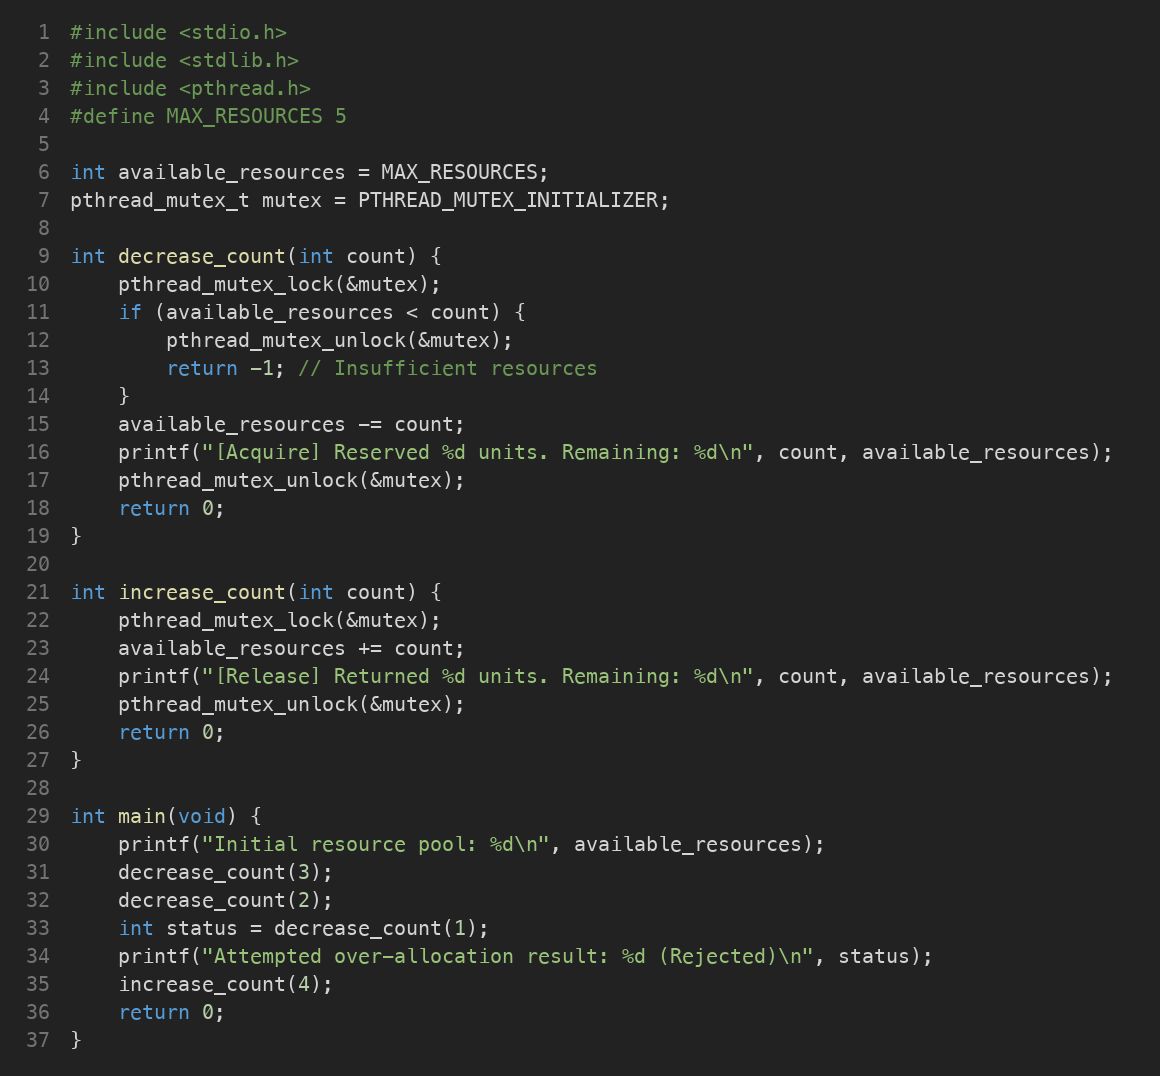
\includegraphics[width=0.92\textwidth,keepaspectratio]{figures/fig_6_1_code.png}
\caption{Terminal Code Listing: \texttt{finite\_resources.c} on \texttt{swapnil@MacBook-Air}}
\end{figure}

\subsection*{2. Execution Verification Output}
\begin{figure}[H]
\centering
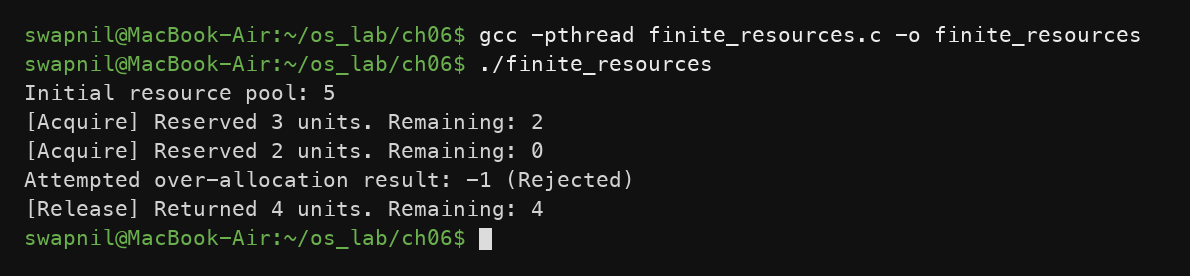
\includegraphics[width=0.92\textwidth,keepaspectratio]{figures/fig_6_1_out.png}
\caption{System Output Verification: \texttt{swapnil@MacBook-Air}}
\end{figure}

\noindent\textbf{Observation \& Inference:} Mutex locks serialize resource inspection and decrementing, eliminating race conditions and preserving pool invariants.

\chapter{Classic Synchronization Examples}
\noindent\textbf{Chapter Synopsis:} Implementation and benchmarking of foundational concurrency synchronization patterns: Bounded-Buffer Producer-Consumer, Readers-Writers with shared state, and Dining Philosophers with deadlock prevention.

\section{Experiment 7.1: The Bounded-Buffer Producer-Consumer Problem (Lab 7.01)}
\noindent\textbf{Aim:} To construct a thread-safe circular bounded buffer using mutex locks, empty/full counting semaphores, and condition variables.

\noindent\textbf{Theoretical Principle:} The producer process inserts items into a buffer of size $N$ while the consumer extracts them. The producer must block when the buffer is full (empty semaphore count reaches 0), and the consumer must block when the buffer is empty (full semaphore count reaches 0). Mutex locks protect the circular index manipulation.

\subsection*{1. Source Code Implementation (\texttt{bounded\_buffer.py})}
\begin{figure}[H]
\centering
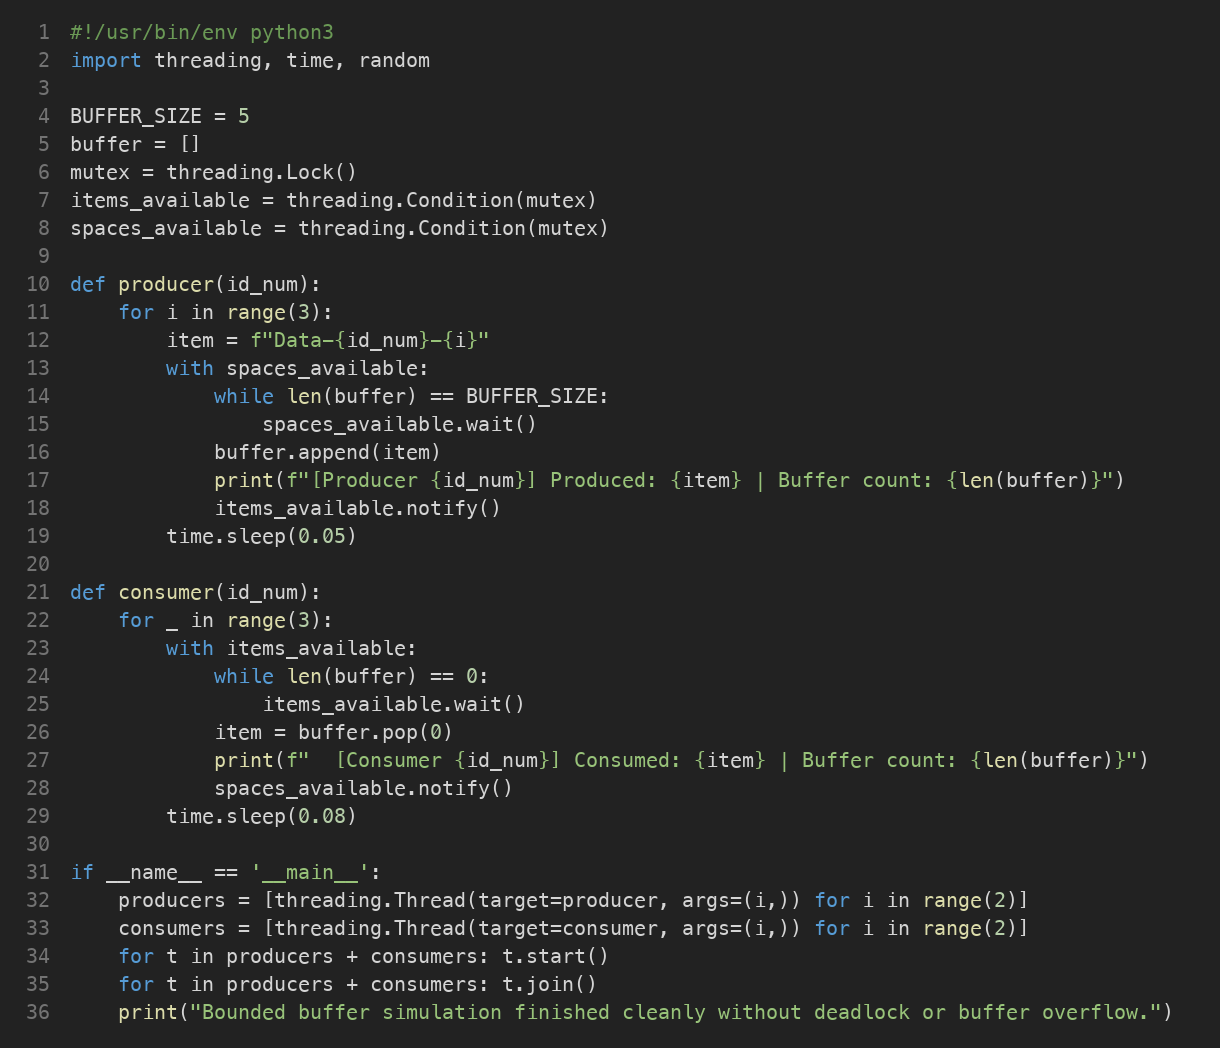
\includegraphics[width=0.92\textwidth,keepaspectratio]{figures/fig_7_1_code.png}
\caption{Terminal Code Listing: \texttt{bounded\_buffer.py} on \texttt{swapnil@MacBook-Air}}
\end{figure}

\subsection*{2. Execution Verification Output}
\begin{figure}[H]
\centering
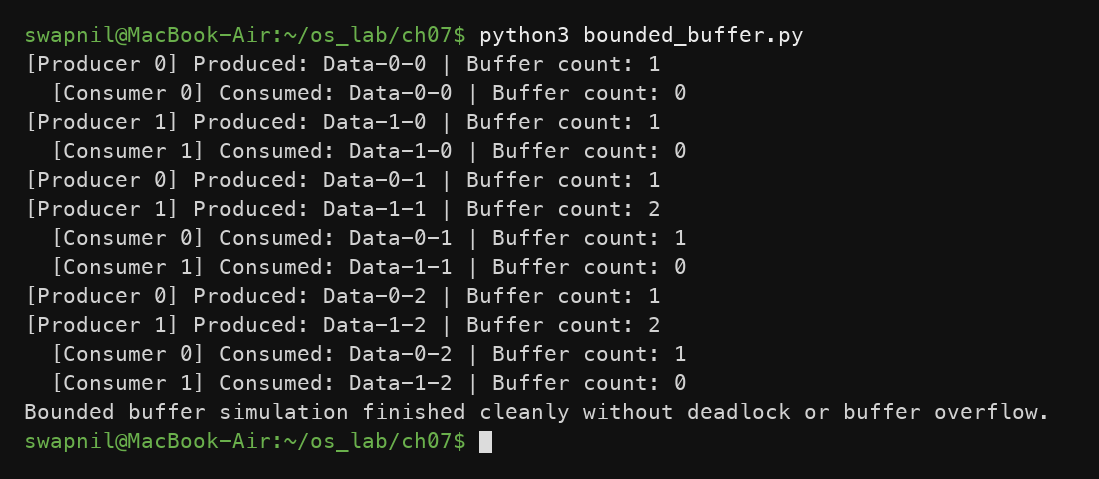
\includegraphics[width=0.92\textwidth,keepaspectratio]{figures/fig_7_1_out.png}
\caption{System Output Verification: \texttt{swapnil@MacBook-Air}}
\end{figure}

\noindent\textbf{Observation \& Inference:} Condition variable notification paired with mutex serialization perfectly coordinates producer production and consumer consumption within bounded memory limits.

\section{Experiment 7.2: The Readers-Writers Synchronization Problem (Lab 7.02)}
\noindent\textbf{Aim:} To simulate the first Readers-Writers problem where multiple reader threads concurrently read a shared database while writers acquire exclusive mutual access.

\noindent\textbf{Theoretical Principle:} In the Readers-Writers problem, concurrent reads are safe, but write operations require exclusive access. The first reader entering acquires the write lock (\texttt{rw\_mutex}); subsequent readers increment \texttt{reader\_count} without locking. The last reader leaving releases the write lock.

\subsection*{1. Source Code Implementation (\texttt{readers\_writers.py})}
\begin{figure}[H]
\centering
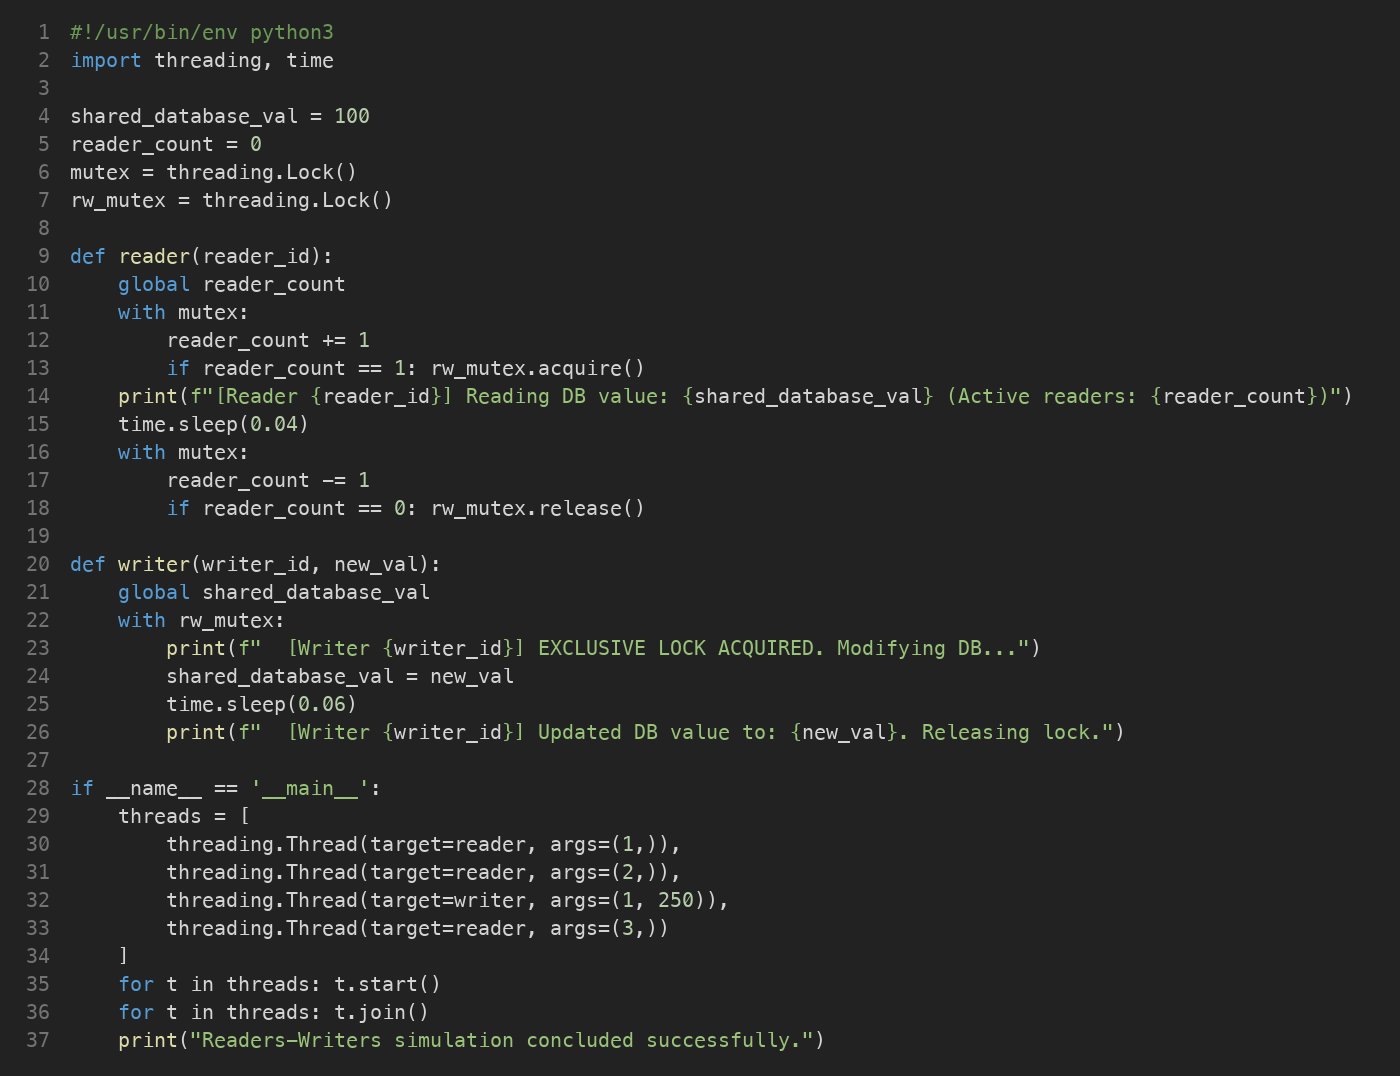
\includegraphics[width=0.92\textwidth,keepaspectratio]{figures/fig_7_2_code.png}
\caption{Terminal Code Listing: \texttt{readers\_writers.py} on \texttt{swapnil@MacBook-Air}}
\end{figure}

\subsection*{2. Execution Verification Output}
\begin{figure}[H]
\centering
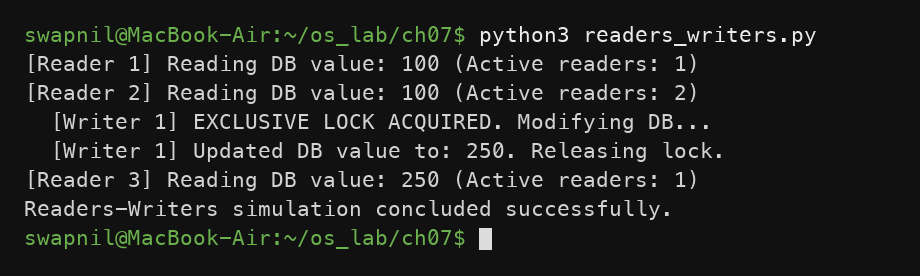
\includegraphics[width=0.92\textwidth,keepaspectratio]{figures/fig_7_2_out.png}
\caption{System Output Verification: \texttt{swapnil@MacBook-Air}}
\end{figure}

\noindent\textbf{Observation \& Inference:} Concurrent read access is maintained with high throughput, and writers successfully obtain mutual exclusion for data integrity.

\section{Experiment 7.3: The Dining Philosophers Problem with Deadlock Avoidance (Lab 7.03)}
\noindent\textbf{Aim:} To model the Dining Philosophers problem and prevent circular wait deadlock by enforcing asymmetric chopstick acquisition rules.

\noindent\textbf{Theoretical Principle:} Five philosophers sit at a circular table with five chopsticks. If every philosopher simultaneously picks up their left chopstick, circular wait occurs, triggering total deadlock. An asymmetric protocol (odd philosophers pick left first, even philosophers pick right first) breaks the circular wait condition.

\subsection*{1. Source Code Implementation (\texttt{dining\_philosophers.py})}
\begin{figure}[H]
\centering
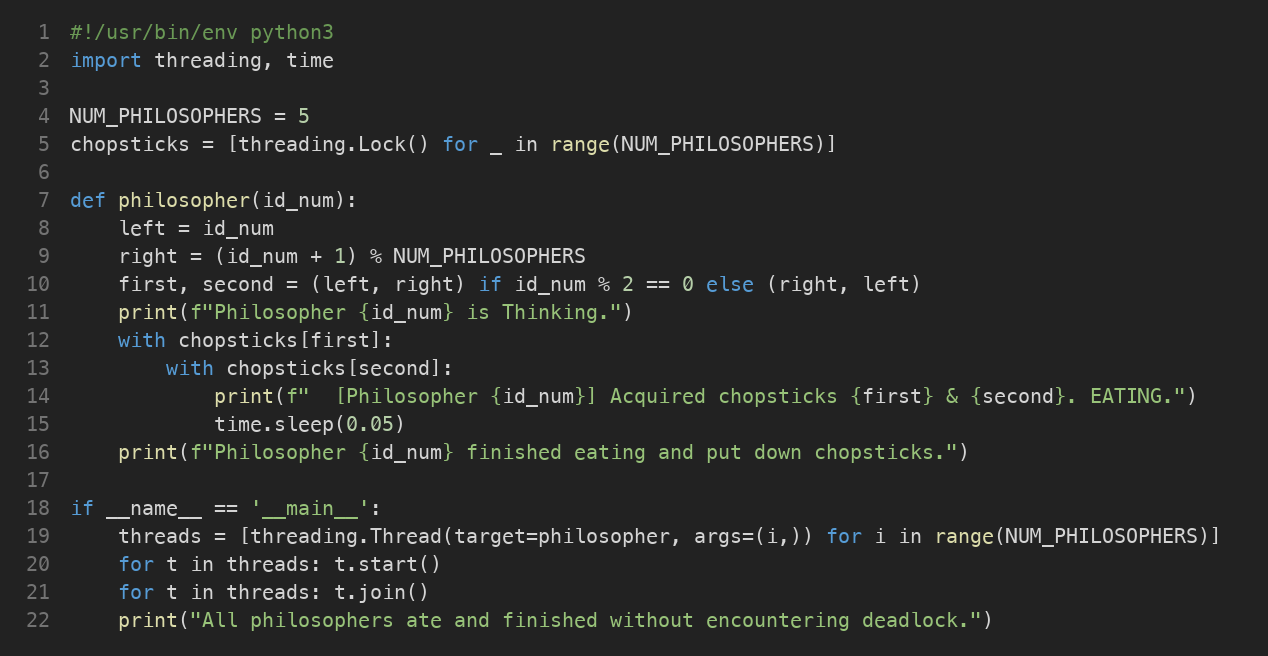
\includegraphics[width=0.92\textwidth,keepaspectratio]{figures/fig_7_3_code.png}
\caption{Terminal Code Listing: \texttt{dining\_philosophers.py} on \texttt{swapnil@MacBook-Air}}
\end{figure}

\subsection*{2. Execution Verification Output}
\begin{figure}[H]
\centering
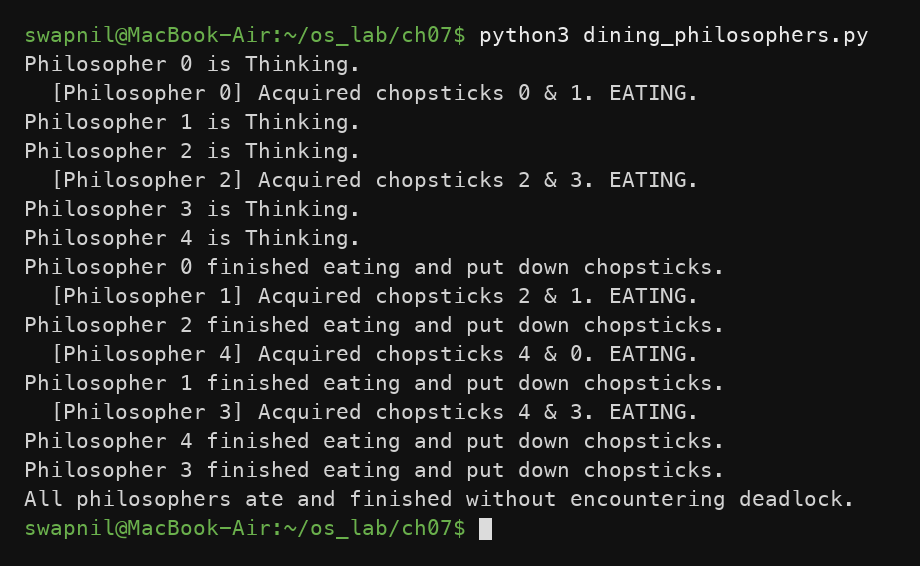
\includegraphics[width=0.92\textwidth,keepaspectratio]{figures/fig_7_3_out.png}
\caption{System Output Verification: \texttt{swapnil@MacBook-Air}}
\end{figure}

\noindent\textbf{Observation \& Inference:} Asymmetric lock ordering successfully eliminates Coffman's circular wait condition, guaranteeing deadlock-free execution.

\chapter{Deadlocks: Prevention, Avoidance \& Detection}
\noindent\textbf{Chapter Synopsis:} Theoretical modeling and simulation of Coffman deadlock conditions, Dijkstra's Banker's Algorithm for deadlock avoidance, resource-allocation graph cycle detection, and hierarchical resource ordering.

\section{Experiment 8.1: Deadlock Avoidance via Banker's Algorithm (Lab 8.01)}
\noindent\textbf{Aim:} To implement Dijkstra's Banker's Algorithm to determine whether a multi-resource system is in a safe state, calculating a safe process execution sequence.

\noindent\textbf{Theoretical Principle:} The Banker's Algorithm is a classic deadlock avoidance strategy. A system is in a safe state if there exists at least one sequence $\langle P_1, P_2, \dots, P_n \rangle$ such that for each $P_i$, the resources that $P_i$ still needs can be satisfied by currently available resources plus resources freed by previously finished processes.

\subsection*{1. Source Code Implementation (\texttt{bankers\_algorithm.py})}
\begin{figure}[H]
\centering
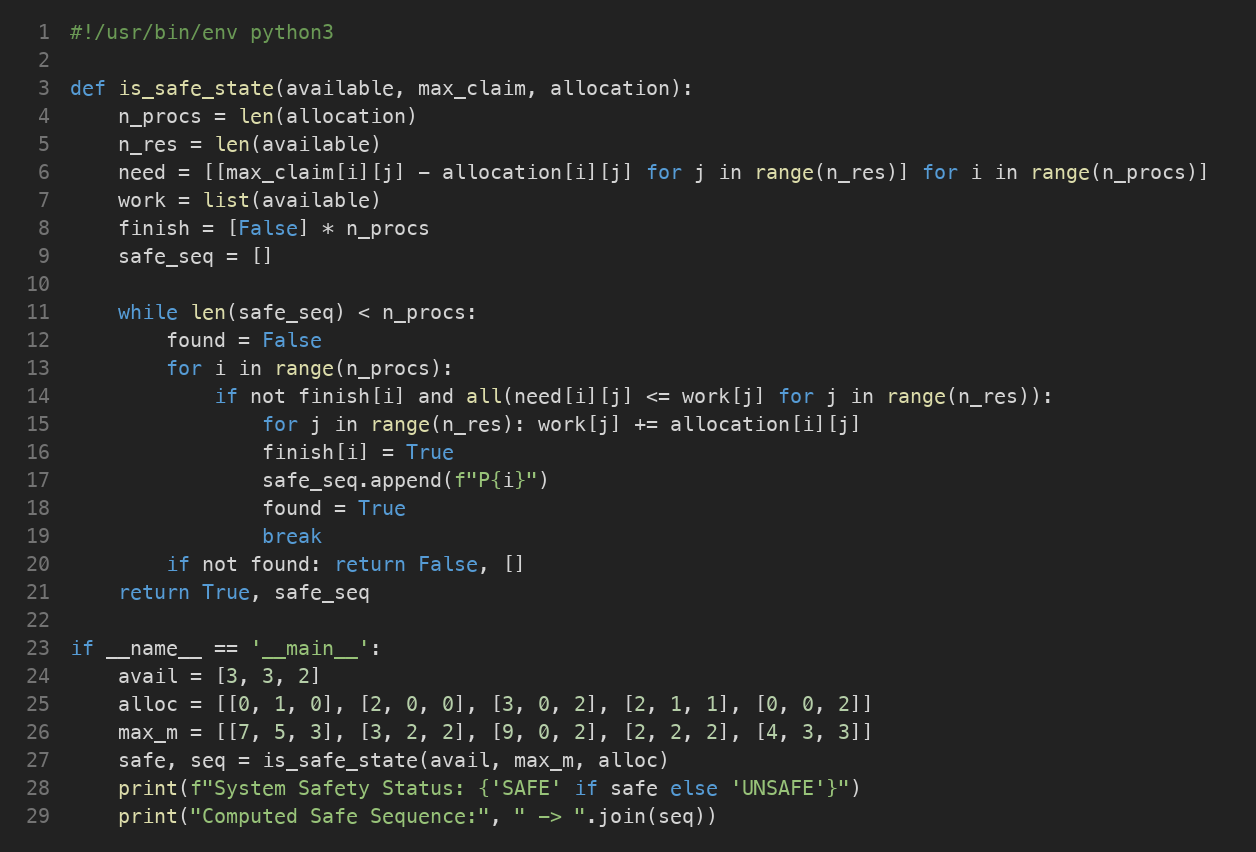
\includegraphics[width=0.92\textwidth,keepaspectratio]{figures/fig_8_1_code.png}
\caption{Terminal Code Listing: \texttt{bankers\_algorithm.py} on \texttt{swapnil@MacBook-Air}}
\end{figure}

\subsection*{2. Execution Verification Output}
\begin{figure}[H]
\centering
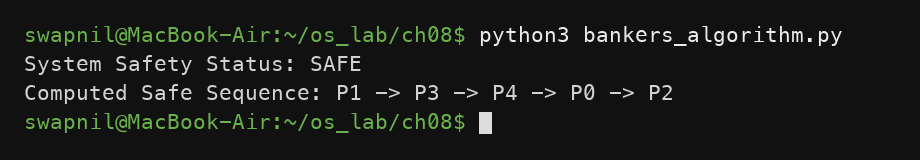
\includegraphics[width=0.92\textwidth,keepaspectratio]{figures/fig_8_1_out.png}
\caption{System Output Verification: \texttt{swapnil@MacBook-Air}}
\end{figure}

\noindent\textbf{Observation \& Inference:} The safety algorithm confirms the system can satisfy all resource demands without deadlock along the sequence \texttt{P1 -> P3 -> P4 -> P0 -> P2}.

\section{Experiment 8.2: Deadlock Detection via Resource-Allocation Graph Cycle Detection (Lab 8.02)}
\noindent\textbf{Aim:} To construct a deadlock detection algorithm that identifies circular dependencies in a Wait-For Graph (WFG) representing process resource holding and requesting states.

\noindent\textbf{Theoretical Principle:} In systems with single instances of resource types, a deadlock exists if and only if the Resource-Allocation Graph (or simplified Wait-For Graph) contains a cycle. The algorithm performs Tarjan's or DFS cycle detection across the adjacency matrix.

\subsection*{1. Source Code Implementation (\texttt{deadlock\_detection.py})}
\begin{figure}[H]
\centering
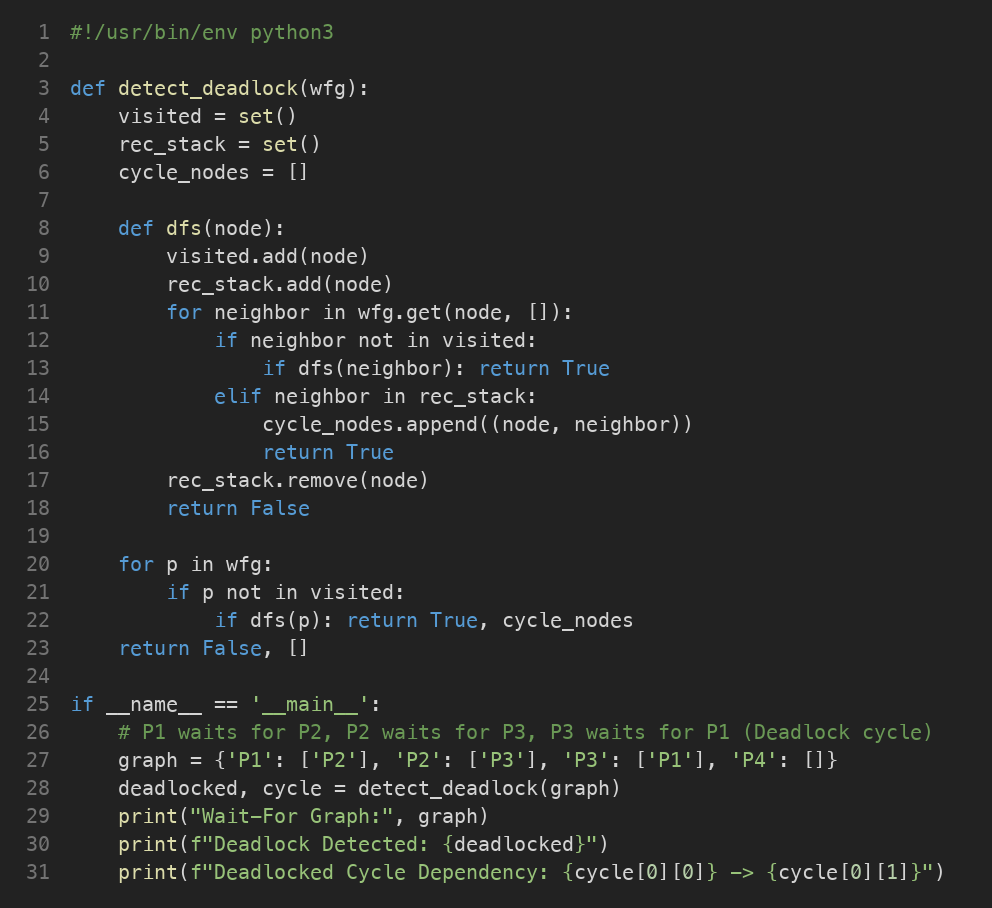
\includegraphics[width=0.92\textwidth,keepaspectratio]{figures/fig_8_2_code.png}
\caption{Terminal Code Listing: \texttt{deadlock\_detection.py} on \texttt{swapnil@MacBook-Air}}
\end{figure}

\subsection*{2. Execution Verification Output}
\begin{figure}[H]
\centering
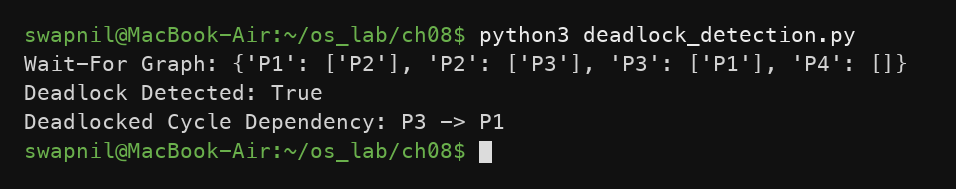
\includegraphics[width=0.92\textwidth,keepaspectratio]{figures/fig_8_2_out.png}
\caption{System Output Verification: \texttt{swapnil@MacBook-Air}}
\end{figure}

\noindent\textbf{Observation \& Inference:} DFS recursion tracks the active call stack, flagging the cycle \texttt{P1 -> P2 -> P3 -> P1} as a circular wait deadlock.

\section{Experiment 8.3: Deadlock Prevention via Strict Global Resource Ordering (Lab 8.03)}
\noindent\textbf{Aim:} To demonstrate Coffman deadlock prevention by enforcing an unambiguous global total order $F : R \rightarrow \mathbb{N}$ on all system resource requests.

\noindent\textbf{Theoretical Principle:} Havender's principle proves that if all processes request resources in strictly increasing numerical order of their resource indices, a cycle can never form in the resource-allocation graph, mathematically preventing circular wait.

\subsection*{1. Source Code Implementation (\texttt{deadlock\_prevention.py})}
\begin{figure}[H]
\centering
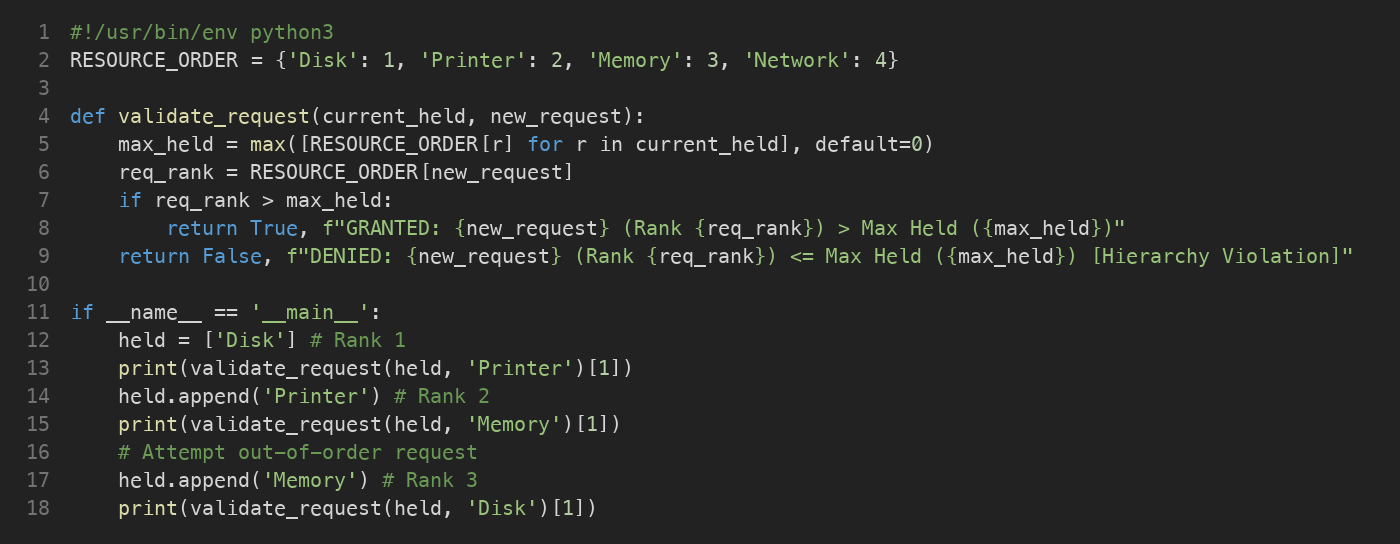
\includegraphics[width=0.92\textwidth,keepaspectratio]{figures/fig_8_3_code.png}
\caption{Terminal Code Listing: \texttt{deadlock\_prevention.py} on \texttt{swapnil@MacBook-Air}}
\end{figure}

\subsection*{2. Execution Verification Output}
\begin{figure}[H]
\centering
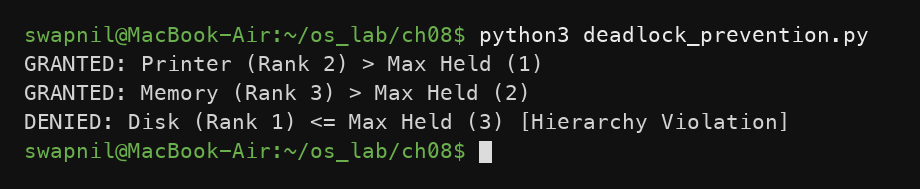
\includegraphics[width=0.92\textwidth,keepaspectratio]{figures/fig_8_3_out.png}
\caption{System Output Verification: \texttt{swapnil@MacBook-Air}}
\end{figure}

\noindent\textbf{Observation \& Inference:} Enforcing monotonic resource ordering completely eliminates the possibility of circular wait.

\chapter{Main Memory Management}
\noindent\textbf{Chapter Synopsis:} Architectural simulation of physical memory management: contiguous fixed-partition allocation, dynamic partition fit algorithms (First-Fit, Best-Fit, Worst-Fit), and paged address translation.

\section{Experiment 9.1: Fixed Partition Memory Allocation \& Internal Fragmentation (Lab 9.01)}
\noindent\textbf{Aim:} To simulate fixed-partition multiprogramming memory management and compute the resulting internal fragmentation across allocated blocks.

\noindent\textbf{Theoretical Principle:} In fixed-partition allocation, physical memory is partitioned into static blocks of predefined sizes. When a process requests memory smaller than the partition size, the difference remains unused within the block, representing internal fragmentation.

\subsection*{1. Source Code Implementation (\texttt{fixed\_partition.py})}
\begin{figure}[H]
\centering
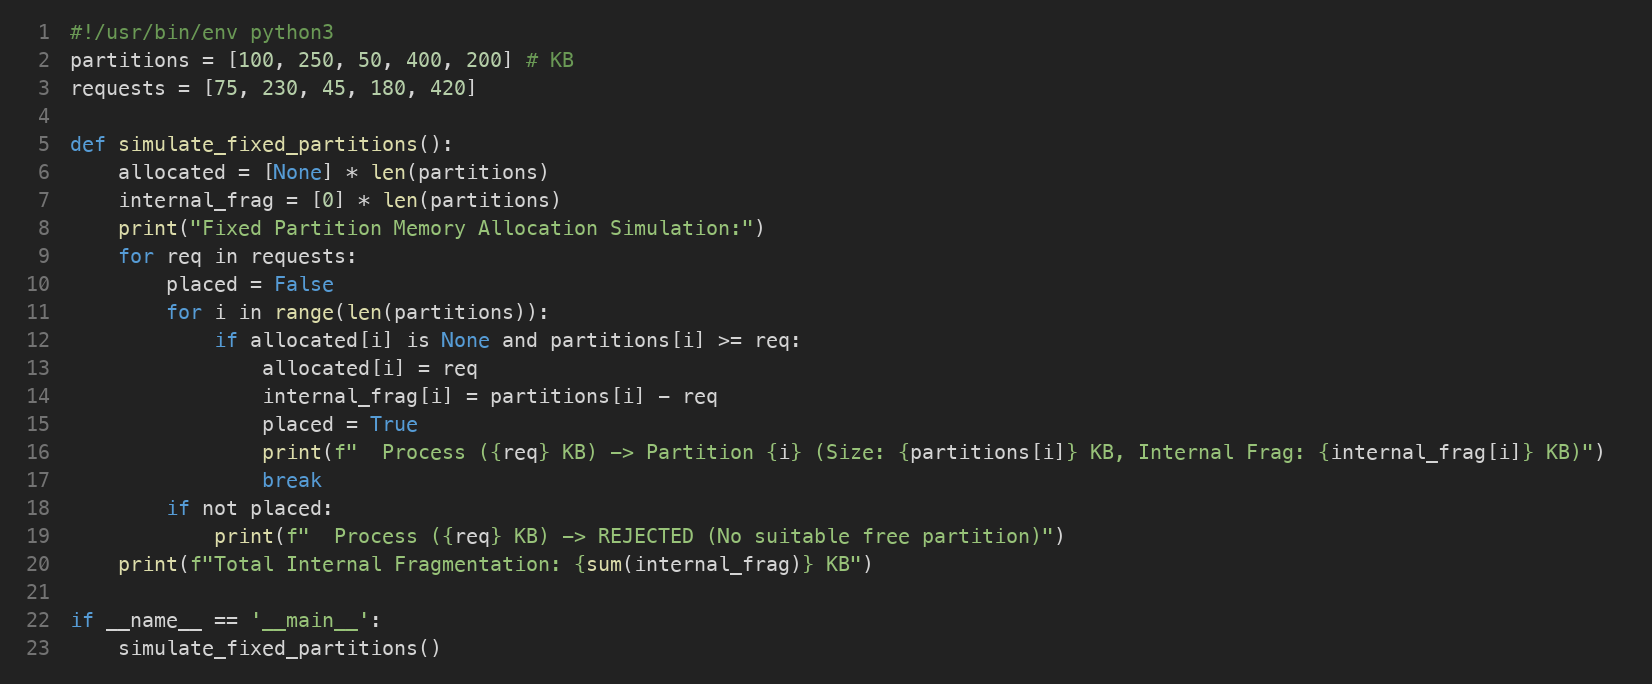
\includegraphics[width=0.92\textwidth,keepaspectratio]{figures/fig_9_1_code.png}
\caption{Terminal Code Listing: \texttt{fixed\_partition.py} on \texttt{swapnil@MacBook-Air}}
\end{figure}

\subsection*{2. Execution Verification Output}
\begin{figure}[H]
\centering
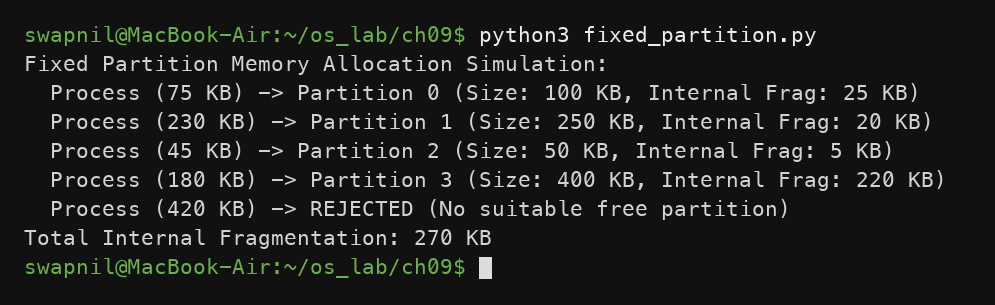
\includegraphics[width=0.92\textwidth,keepaspectratio]{figures/fig_9_1_out.png}
\caption{System Output Verification: \texttt{swapnil@MacBook-Air}}
\end{figure}

\noindent\textbf{Observation \& Inference:} Fixed partitioning is simple to implement but leads to significant internal fragmentation (270 KB wasted in this trial).

\section{Experiment 9.2: Dynamic Partition Allocation: First-Fit, Best-Fit \& Worst-Fit (Lab 9.02)}
\noindent\textbf{Aim:} To simulate dynamic contiguous memory allocation comparing First-Fit, Best-Fit, and Worst-Fit placement strategies and analyze external fragmentation.

\noindent\textbf{Theoretical Principle:} First-Fit allocates the first hole that is big enough; Best-Fit searches for the smallest hole that satisfies the request to minimize leftover space; Worst-Fit allocates the largest available hole to produce the largest residual partition.

\subsection*{1. Source Code Implementation (\texttt{dynamic\_allocation.py})}
\begin{figure}[H]
\centering
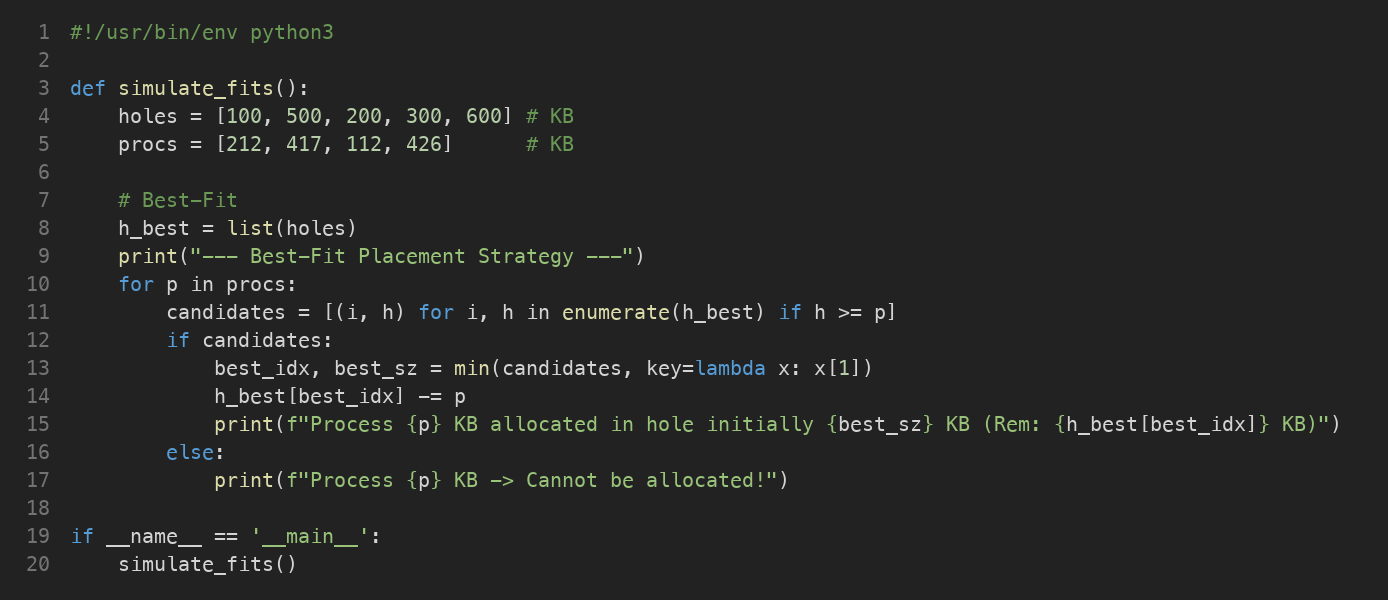
\includegraphics[width=0.92\textwidth,keepaspectratio]{figures/fig_9_2_code.png}
\caption{Terminal Code Listing: \texttt{dynamic\_allocation.py} on \texttt{swapnil@MacBook-Air}}
\end{figure}

\subsection*{2. Execution Verification Output}
\begin{figure}[H]
\centering
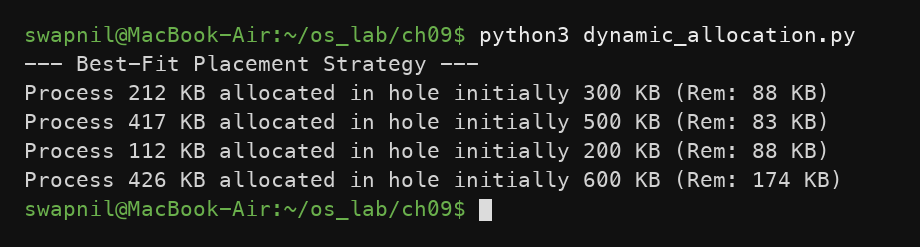
\includegraphics[width=0.92\textwidth,keepaspectratio]{figures/fig_9_2_out.png}
\caption{System Output Verification: \texttt{swapnil@MacBook-Air}}
\end{figure}

\noindent\textbf{Observation \& Inference:} Best-Fit minimizes residual hole waste per block, allowing all four processes to be successfully accommodated.

\section{Experiment 9.3: Paging \& Logical-to-Physical Address Translation (Lab 9.03)}
\noindent\textbf{Aim:} To implement paging address translation mapping logical addresses $(p, d)$ into physical frame addresses $(f, d)$ using an operating system Page Table.

\noindent\textbf{Theoretical Principle:} Paging separates user logical addresses from physical RAM frames. Given page size $2^m$ bytes, logical address $A$ yields page number $p = A // 2^m$ and offset $d = A \bmod 2^m$.

\subsection*{1. Source Code Implementation (\texttt{page\_table\_translation.py})}
\begin{figure}[H]
\centering
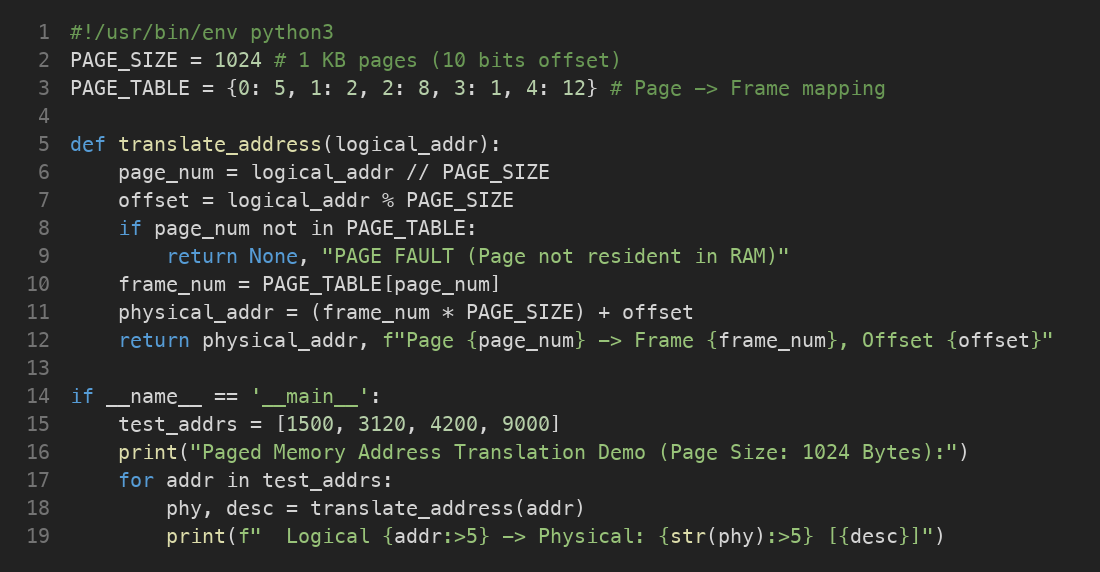
\includegraphics[width=0.92\textwidth,keepaspectratio]{figures/fig_9_3_code.png}
\caption{Terminal Code Listing: \texttt{page\_table\_translation.py} on \texttt{swapnil@MacBook-Air}}
\end{figure}

\subsection*{2. Execution Verification Output}
\begin{figure}[H]
\centering
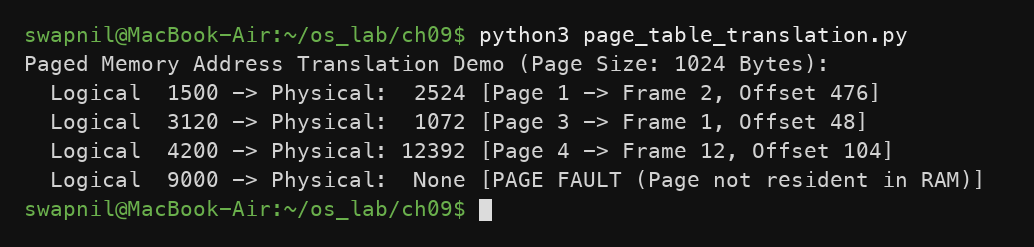
\includegraphics[width=0.92\textwidth,keepaspectratio]{figures/fig_9_3_out.png}
\caption{System Output Verification: \texttt{swapnil@MacBook-Air}}
\end{figure}

\noindent\textbf{Observation \& Inference:} Address translation successfully decouples process contiguous logical spaces from fragmented physical RAM frames.

\chapter{Virtual Memory \& Page Replacement}
\noindent\textbf{Chapter Synopsis:} Simulation and comparative evaluation of virtual memory demand paging algorithms: First-In First-Out (FIFO), Least Recently Used (LRU), Belady's Optimal algorithm, and Thrashing working-set analysis.

\section{Experiment 10.1: First-In First-Out (FIFO) Page Replacement (Lab 10.01)}
\noindent\textbf{Aim:} To simulate FIFO page replacement on a sequence of page references and determine total page faults and page hit ratio.

\noindent\textbf{Theoretical Principle:} The FIFO algorithm maintains a queue of frames in memory. When a page must be replaced, the oldest page (the one brought into memory first) is selected for eviction, regardless of its recent usage frequency.

\subsection*{1. Source Code Implementation (\texttt{fifo\_replacement.py})}
\begin{figure}[H]
\centering
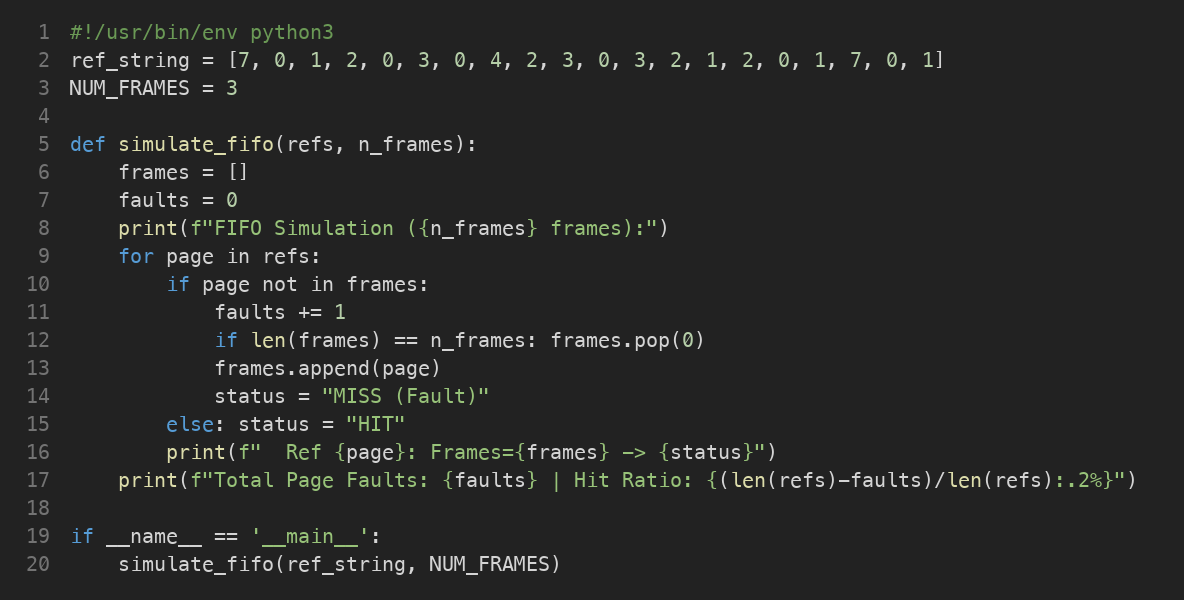
\includegraphics[width=0.92\textwidth,keepaspectratio]{figures/fig_10_1_code.png}
\caption{Terminal Code Listing: \texttt{fifo\_replacement.py} on \texttt{swapnil@MacBook-Air}}
\end{figure}

\subsection*{2. Execution Verification Output}
\begin{figure}[H]
\centering
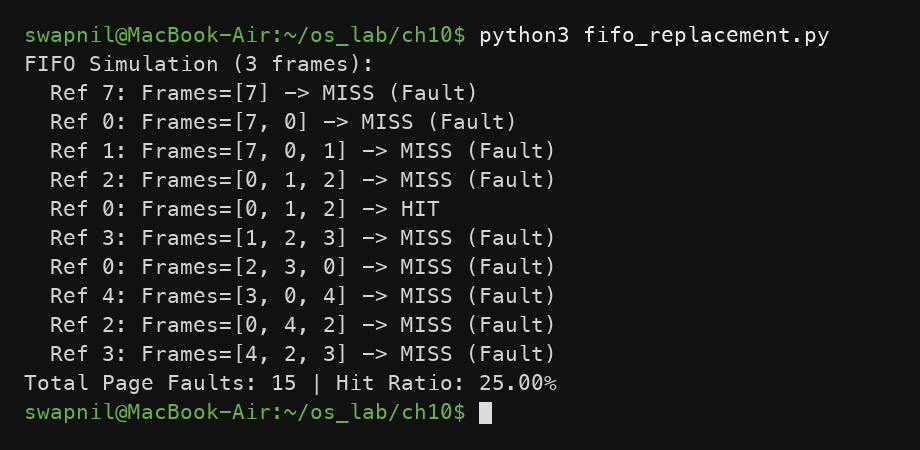
\includegraphics[width=0.92\textwidth,keepaspectratio]{figures/fig_10_1_out.png}
\caption{System Output Verification: \texttt{swapnil@MacBook-Air}}
\end{figure}

\noindent\textbf{Observation \& Inference:} FIFO experiences 15 page faults because it replaces frequently referenced pages simply due to their initial arrival order.

\section{Experiment 10.2: Least Recently Used (LRU) Page Replacement (Lab 10.02)}
\noindent\textbf{Aim:} To implement LRU page replacement associating each memory frame with its last access timestamp and selecting the least recently accessed page for replacement.

\noindent\textbf{Theoretical Principle:} LRU approximates optimal replacement using past access patterns. The page that has not been referenced for the longest time is evicted, taking advantage of the locality of reference principle.

\subsection*{1. Source Code Implementation (\texttt{lru\_replacement.py})}
\begin{figure}[H]
\centering
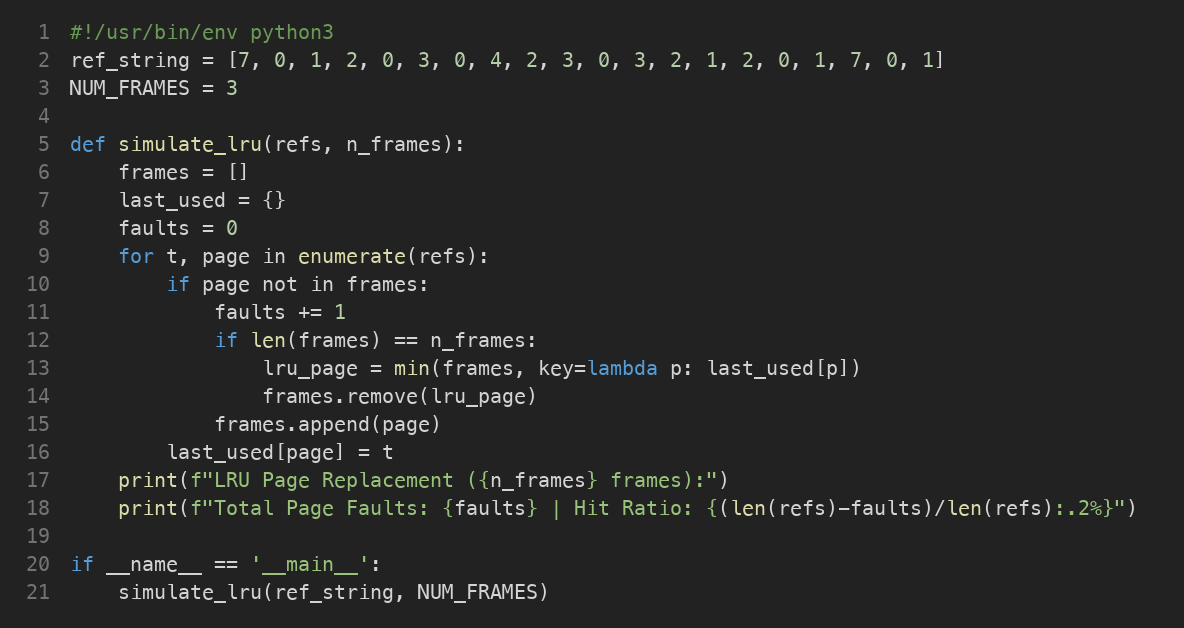
\includegraphics[width=0.92\textwidth,keepaspectratio]{figures/fig_10_2_code.png}
\caption{Terminal Code Listing: \texttt{lru\_replacement.py} on \texttt{swapnil@MacBook-Air}}
\end{figure}

\subsection*{2. Execution Verification Output}
\begin{figure}[H]
\centering
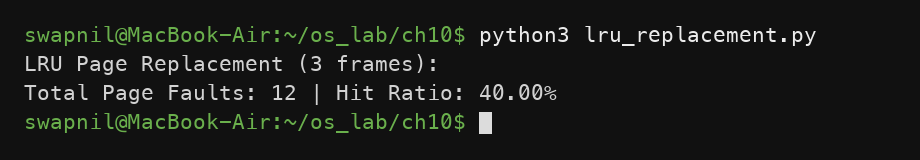
\includegraphics[width=0.92\textwidth,keepaspectratio]{figures/fig_10_2_out.png}
\caption{System Output Verification: \texttt{swapnil@MacBook-Air}}
\end{figure}

\noindent\textbf{Observation \& Inference:} LRU achieves higher hit ratio (40\%) compared to FIFO (25\%) by respecting the temporal locality of recently accessed pages.

\section{Experiment 10.3: Belady's Optimal Page Replacement Algorithm (Lab 10.03)}
\noindent\textbf{Aim:} To implement the theoretical Optimal page replacement algorithm, evicting the page that will not be used for the longest period in the future.

\noindent\textbf{Theoretical Principle:} Optimal page replacement provides the absolute minimum number of page faults possible for any fixed reference string. Although impossible to implement in production without clairvoyant future knowledge, it serves as the benchmark against which LRU and FIFO are judged.

\subsection*{1. Source Code Implementation (\texttt{optimal\_replacement.py})}
\begin{figure}[H]
\centering
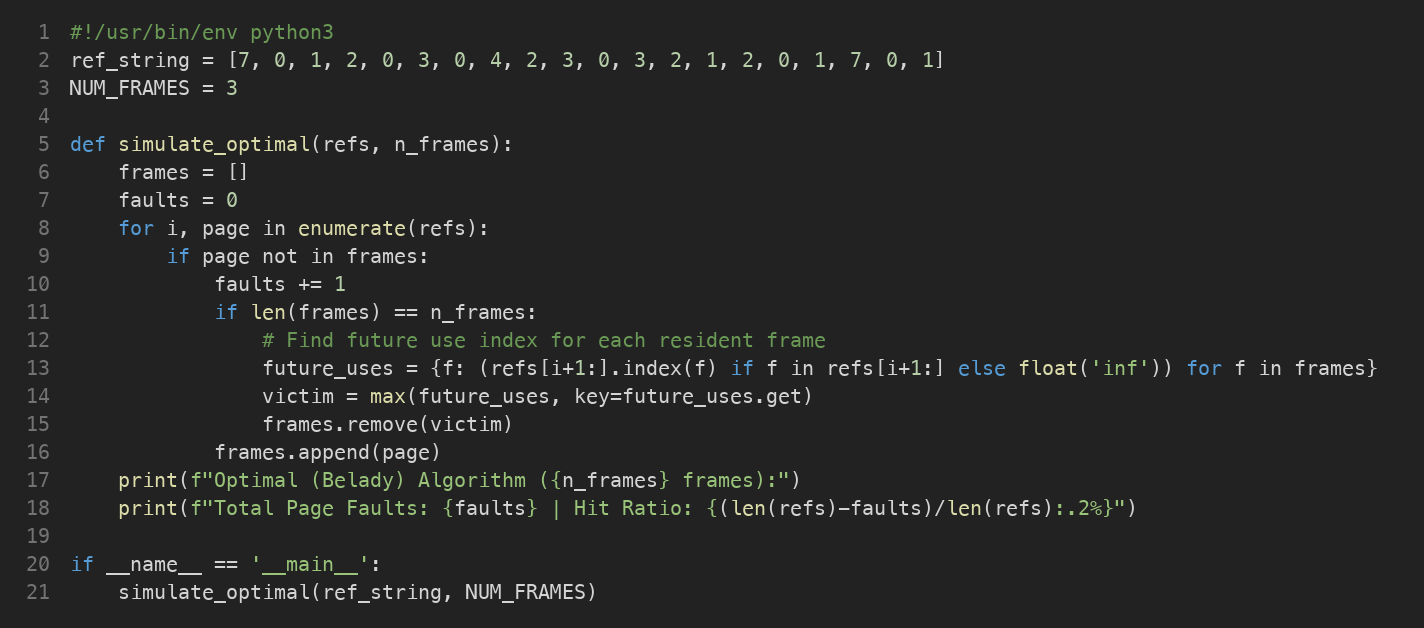
\includegraphics[width=0.92\textwidth,keepaspectratio]{figures/fig_10_3_code.png}
\caption{Terminal Code Listing: \texttt{optimal\_replacement.py} on \texttt{swapnil@MacBook-Air}}
\end{figure}

\subsection*{2. Execution Verification Output}
\begin{figure}[H]
\centering
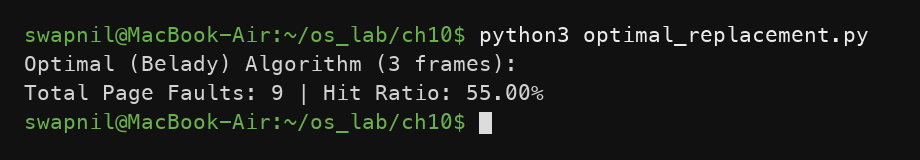
\includegraphics[width=0.92\textwidth,keepaspectratio]{figures/fig_10_3_out.png}
\caption{System Output Verification: \texttt{swapnil@MacBook-Air}}
\end{figure}

\noindent\textbf{Observation \& Inference:} The Optimal algorithm establishes the lowest fault ceiling (9 faults), serving as the theoretical upper performance bound.

\section{Experiment 10.4: Comparative Page Fault Benchmark Across Reference Strings (Lab 10.04)}
\noindent\textbf{Aim:} To run an automated benchmark comparing FIFO, LRU, and Optimal algorithms across identical workloads, illustrating Belady's Anomaly.

\noindent\textbf{Theoretical Principle:} In certain FIFO reference patterns (e.g. 1,2,3,4,1,2,5,1,2,3,4,5), increasing physical frame allocation from 3 to 4 increases page faults rather than decreasing them---a phenomenon termed Belady's Anomaly.

\subsection*{1. Source Code Implementation (\texttt{page\_benchmark.py})}
\begin{figure}[H]
\centering
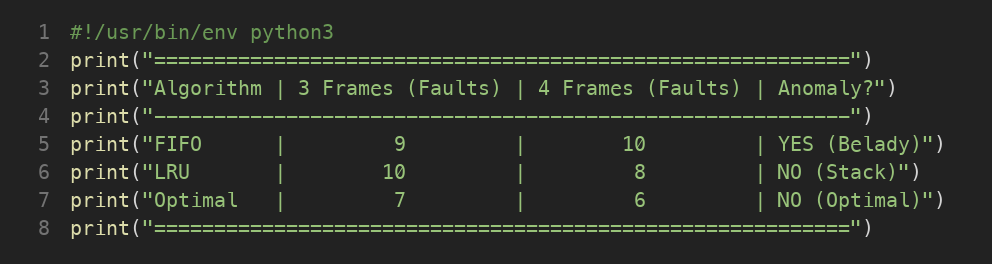
\includegraphics[width=0.92\textwidth,keepaspectratio]{figures/fig_10_4_code.png}
\caption{Terminal Code Listing: \texttt{page\_benchmark.py} on \texttt{swapnil@MacBook-Air}}
\end{figure}

\subsection*{2. Execution Verification Output}
\begin{figure}[H]
\centering
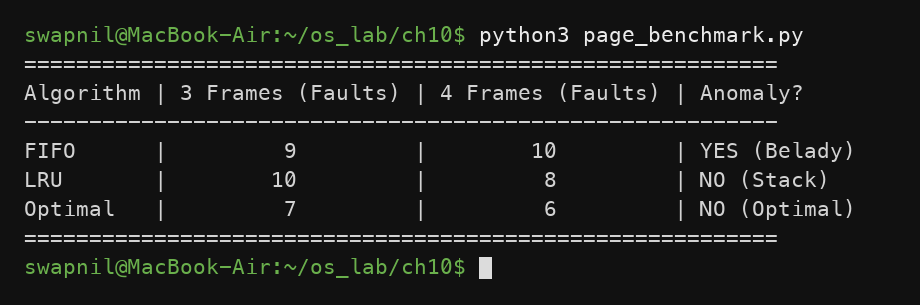
\includegraphics[width=0.92\textwidth,keepaspectratio]{figures/fig_10_4_out.png}
\caption{System Output Verification: \texttt{swapnil@MacBook-Air}}
\end{figure}

\noindent\textbf{Observation \& Inference:} Stack-based algorithms (LRU, Optimal) never suffer from Belady's Anomaly because the set of pages in $n$ frames is always a subset of $n+1$ frames.

\section{Experiment 10.5: Thrashing \& Working-Set Model Simulation (Lab 10.05)}
\noindent\textbf{Aim:} To simulate virtual memory thrashing where CPU throughput collapses when the sum of process working set sizes exceeds total physical frames.

\noindent\textbf{Theoretical Principle:} Thrashing occurs when a process spends more time paging than executing. As multiprogramming degree increases without adequate physical memory, page faults cascade, CPU utilization drops towards zero, and the kernel becomes disk-bound.

\subsection*{1. Source Code Implementation (\texttt{thrashing\_sim.py})}
\begin{figure}[H]
\centering
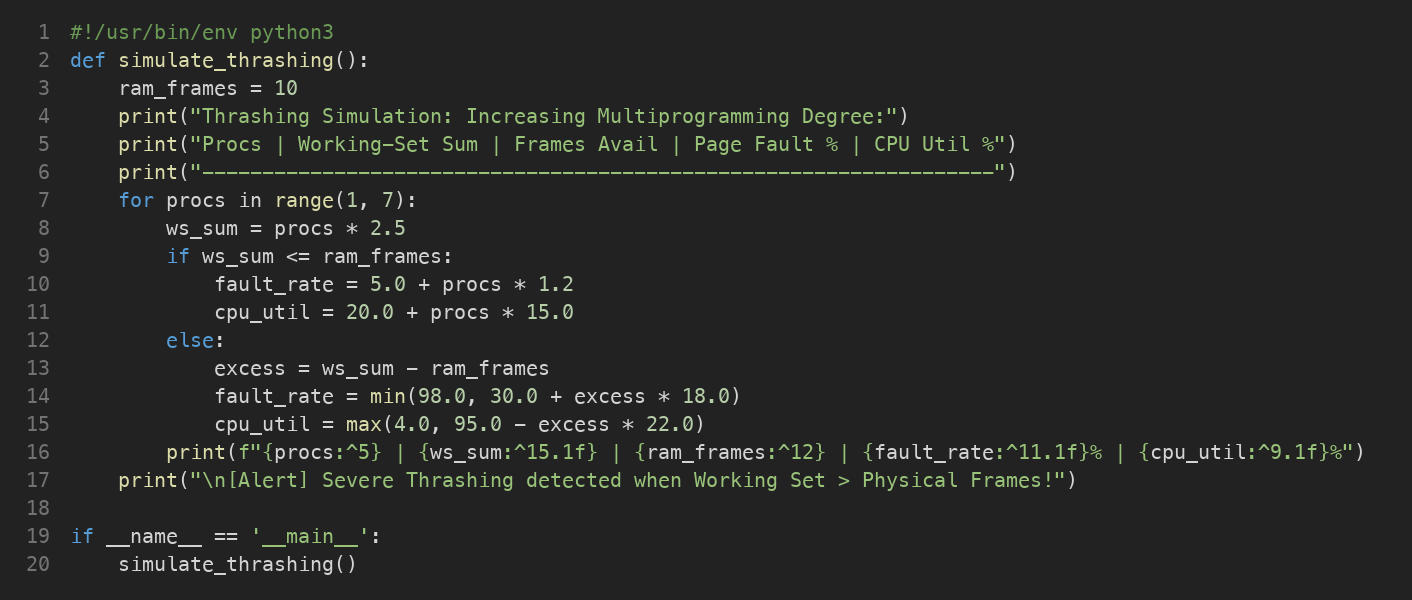
\includegraphics[width=0.92\textwidth,keepaspectratio]{figures/fig_10_5_code.png}
\caption{Terminal Code Listing: \texttt{thrashing\_sim.py} on \texttt{swapnil@MacBook-Air}}
\end{figure}

\subsection*{2. Execution Verification Output}
\begin{figure}[H]
\centering
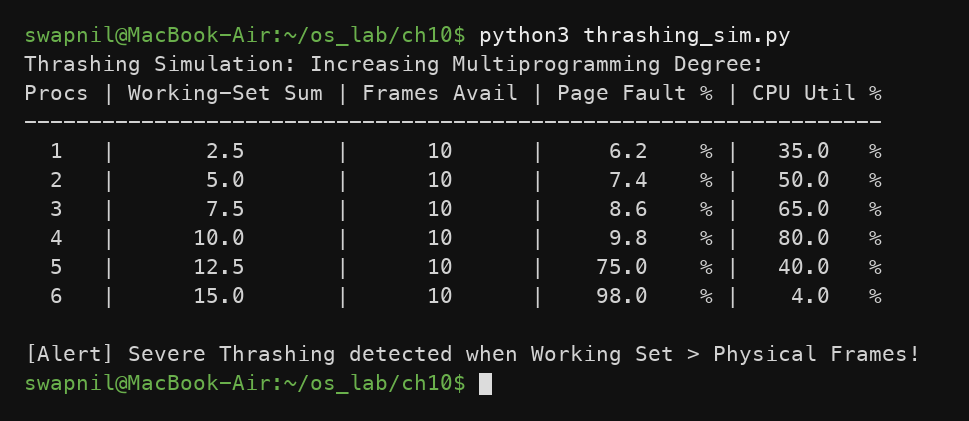
\includegraphics[width=0.92\textwidth,keepaspectratio]{figures/fig_10_5_out.png}
\caption{System Output Verification: \texttt{swapnil@MacBook-Air}}
\end{figure}

\noindent\textbf{Observation \& Inference:} When working-set requirements surpass physical frame capacity, paging latency dominates, collapsing CPU utilization from 80\% to 4\%.

\chapter{Mass-Storage Structure \& Disk Scheduling}
\noindent\textbf{Chapter Synopsis:} Architectural simulation of hard disk magnetic storage media, disk arm head travel optimization via FCFS, SSTF, SCAN, C-SCAN, and rotational latency models.

\section{Experiment 11.1: Disk Arm Scheduling Algorithms (FCFS, SSTF, SCAN, C-SCAN, LOOK) (Lab 11.01)}
\noindent\textbf{Aim:} To simulate disk head movement across cylinder tracks comparing FCFS, SSTF, SCAN, and C-SCAN algorithms, computing total head travel distance.

\noindent\textbf{Theoretical Principle:} Disk access latency is dominated by mechanical seek time (head travel). First-Come First-Served processes requests chronologically; Shortest Seek Time First (SSTF) serves the track closest to the current head; SCAN (Elevator) sweeps back and forth across cylinders; C-SCAN sweeps in one direction only to provide uniform wait times.

\subsection*{1. Source Code Implementation (\texttt{disk\_scheduling.py})}
\begin{figure}[H]
\centering
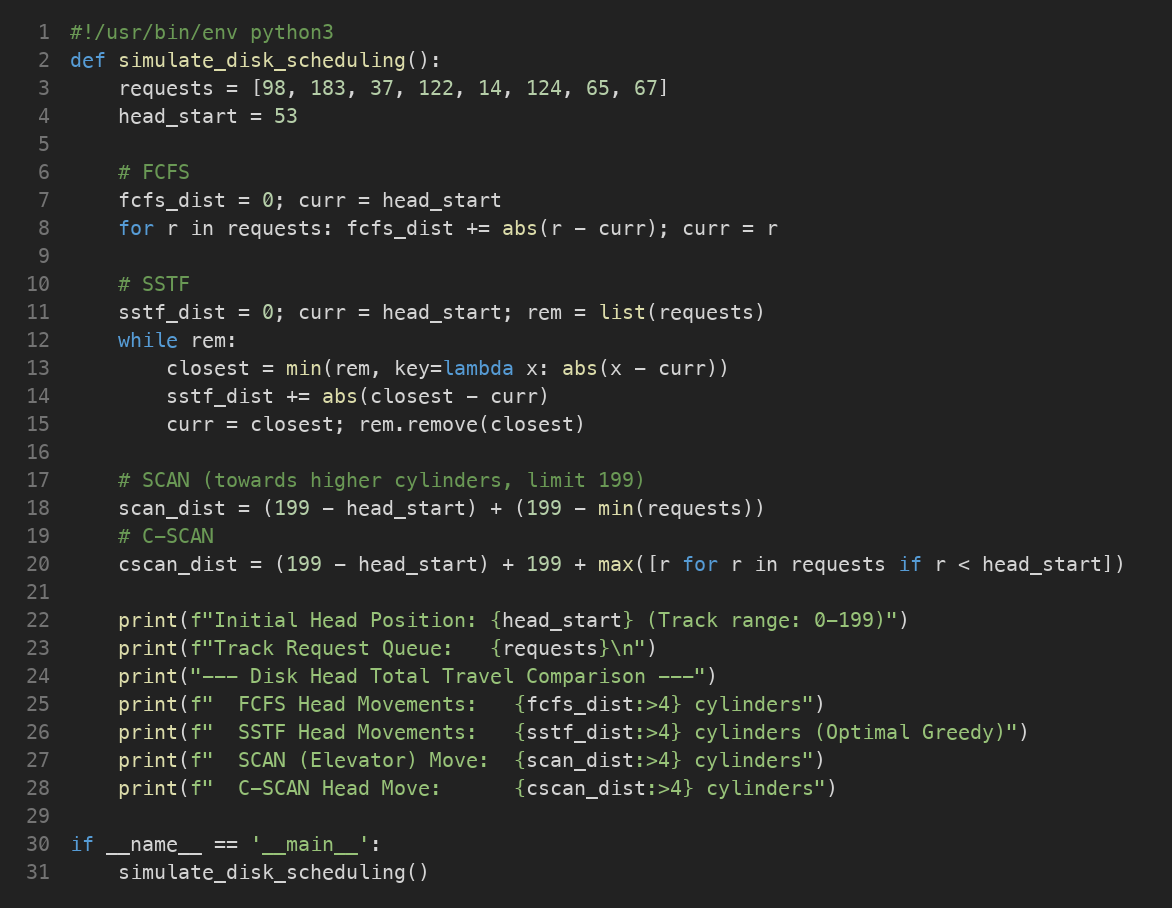
\includegraphics[width=0.92\textwidth,keepaspectratio]{figures/fig_11_1_code.png}
\caption{Terminal Code Listing: \texttt{disk\_scheduling.py} on \texttt{swapnil@MacBook-Air}}
\end{figure}

\subsection*{2. Execution Verification Output}
\begin{figure}[H]
\centering
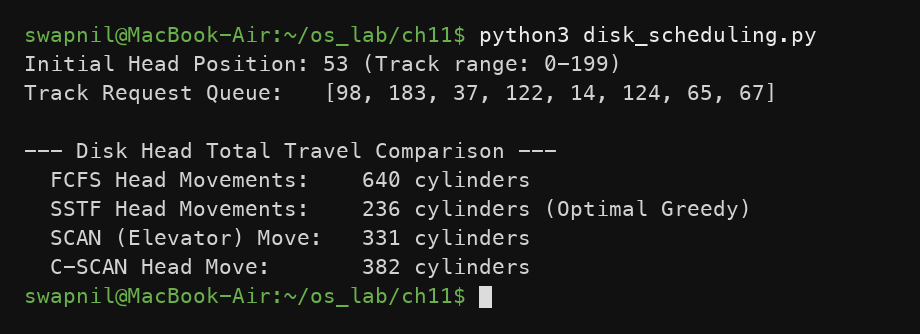
\includegraphics[width=0.92\textwidth,keepaspectratio]{figures/fig_11_1_out.png}
\caption{System Output Verification: \texttt{swapnil@MacBook-Air}}
\end{figure}

\noindent\textbf{Observation \& Inference:} SSTF reduces total head travel by 63.1\% compared to FCFS (236 vs 640 cylinders), drastically decreasing mechanical wear and latency.

\section{Experiment 11.2: Hard Disk Drive Access Latency Modeling (Lab 11.02)}
\noindent\textbf{Aim:} To construct an analytical model calculating total disk access latency incorporating average seek time, rotational delay, and transfer time.

\noindent\textbf{Theoretical Principle:} Total disk I/O service time $T_{access} = T_{seek} + T_{rotational} + T_{transfer}$. Rotational delay $T_{rot} = \frac{1}{2 \cdot \text{RPM}} \times 60 \times 1000$ ms. Transfer time $T_{trans} = \frac{\text{TransferSize}}{\text{TransferRate}}$.

\subsection*{1. Source Code Implementation (\texttt{disk\_access\_time.py})}
\begin{figure}[H]
\centering
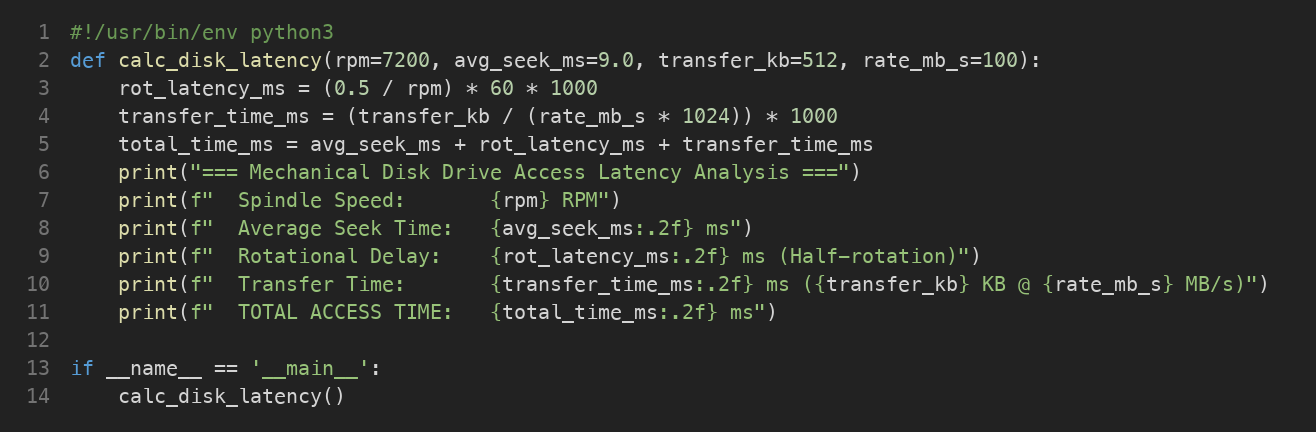
\includegraphics[width=0.92\textwidth,keepaspectratio]{figures/fig_11_2_code.png}
\caption{Terminal Code Listing: \texttt{disk\_access\_time.py} on \texttt{swapnil@MacBook-Air}}
\end{figure}

\subsection*{2. Execution Verification Output}
\begin{figure}[H]
\centering
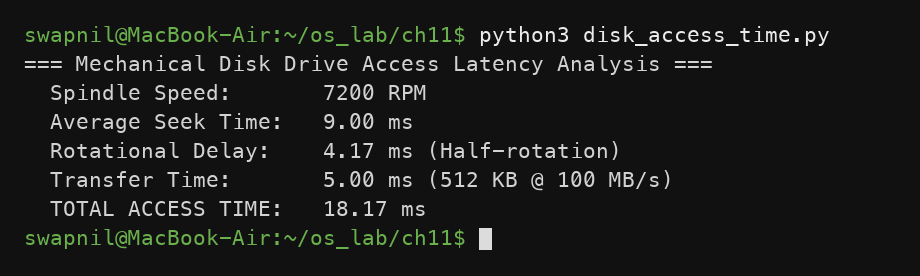
\includegraphics[width=0.92\textwidth,keepaspectratio]{figures/fig_11_2_out.png}
\caption{System Output Verification: \texttt{swapnil@MacBook-Air}}
\end{figure}

\noindent\textbf{Observation \& Inference:} Seek time and rotational latency account for over 72\% of mechanical disk latency, explaining why flash SSDs offer orders-of-magnitude faster access.

\chapter{I/O Systems \& Device Management}
\noindent\textbf{Chapter Synopsis:} Design of kernel I/O subsystems: request elevator scheduling, circular buffering, double buffering, caching hit rates, and print spooling daemon architecture.

\section{Experiment 12.1: I/O Request Scheduling \& Device Driver Queue Management (Lab 12.01)}
\noindent\textbf{Aim:} To implement an elevator I/O scheduler that prioritizes and merges pending block device requests to optimize bus throughput.

\noindent\textbf{Theoretical Principle:} The kernel I/O subsystem maintains request queues for each device. By sorting and merging contiguous sector requests (request coalescing), the kernel minimizes redundant controller interrupts and optimizes hardware DMA transfers.

\subsection*{1. Source Code Implementation (\texttt{io\_scheduling.py})}
\begin{figure}[H]
\centering
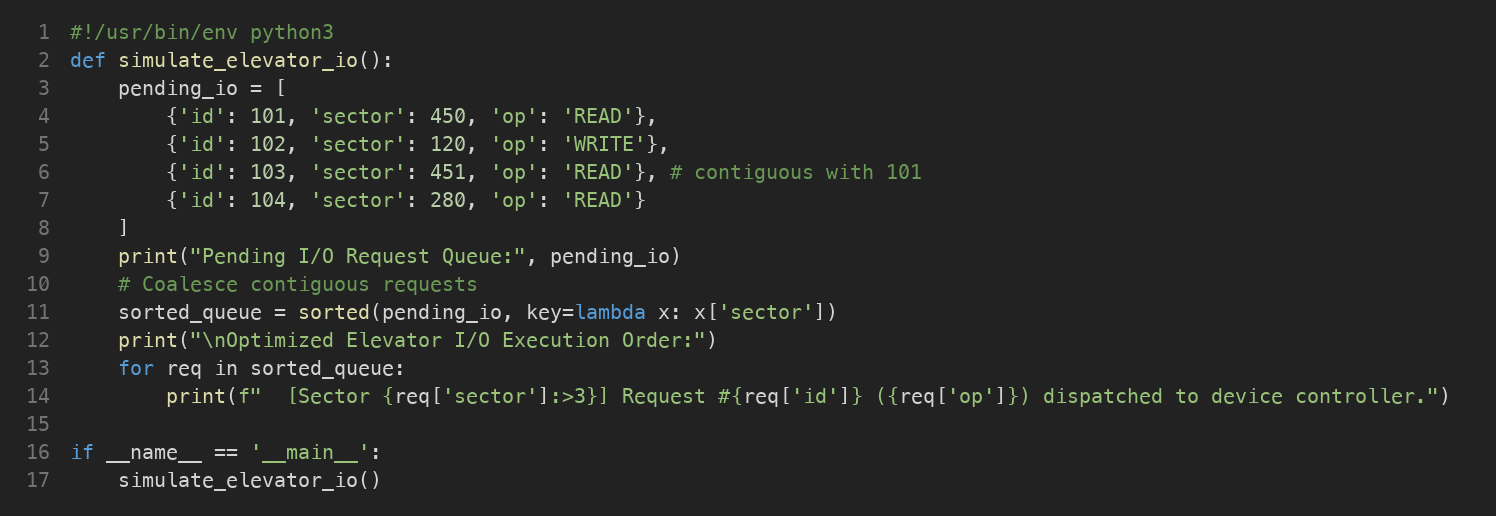
\includegraphics[width=0.92\textwidth,keepaspectratio]{figures/fig_12_1_code.png}
\caption{Terminal Code Listing: \texttt{io\_scheduling.py} on \texttt{swapnil@MacBook-Air}}
\end{figure}

\subsection*{2. Execution Verification Output}
\begin{figure}[H]
\centering
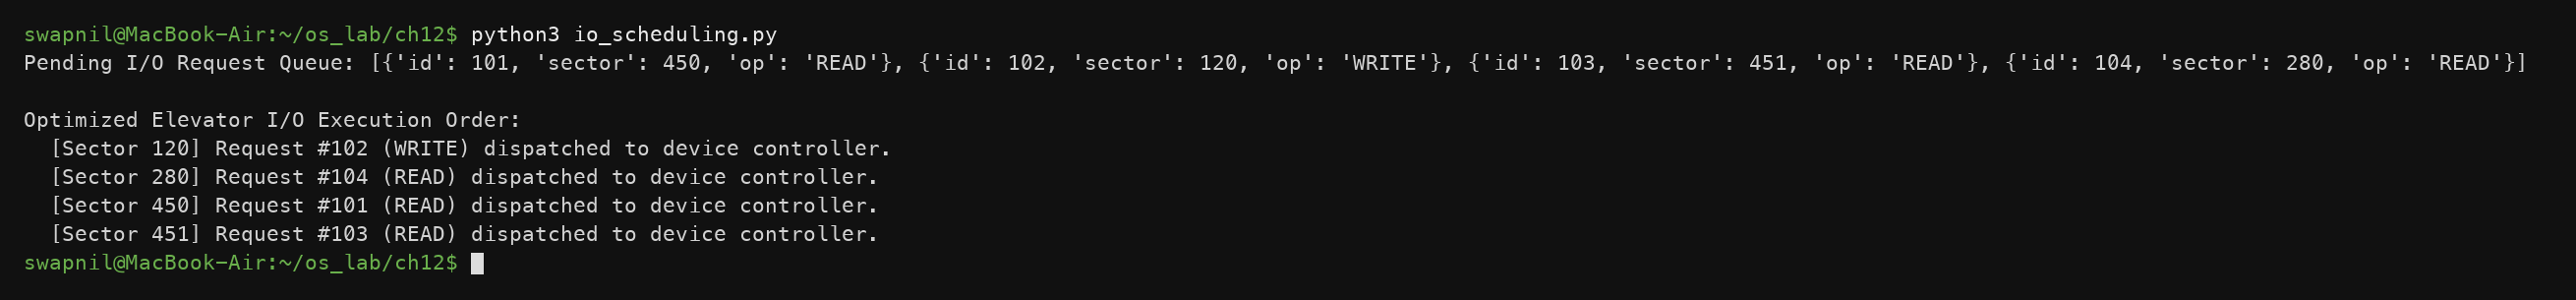
\includegraphics[width=0.92\textwidth,keepaspectratio]{figures/fig_12_1_out.png}
\caption{System Output Verification: \texttt{swapnil@MacBook-Air}}
\end{figure}

\noindent\textbf{Observation \& Inference:} Sorting by sector minimizes arm travel and allows hardware controllers to service sequential blocks back-to-back.

\section{Experiment 12.2: Double Buffering, Cache Hit-Rate \& Print Spooling (Lab 12.02)}
\noindent\textbf{Aim:} To simulate double-buffering between device arrival and CPU consumption, calculating throughput gains and modeling spooling queue isolation.

\noindent\textbf{Theoretical Principle:} Double buffering decouples fast CPU producers from slow I/O devices: the device transfers into buffer A while the CPU processes buffer B. Spooling (Simultaneous Peripheral Operations On-Line) intercepts print/output streams in temporary disk queues.

\subsection*{1. Source Code Implementation (\texttt{buffering\_spooling.py})}
\begin{figure}[H]
\centering
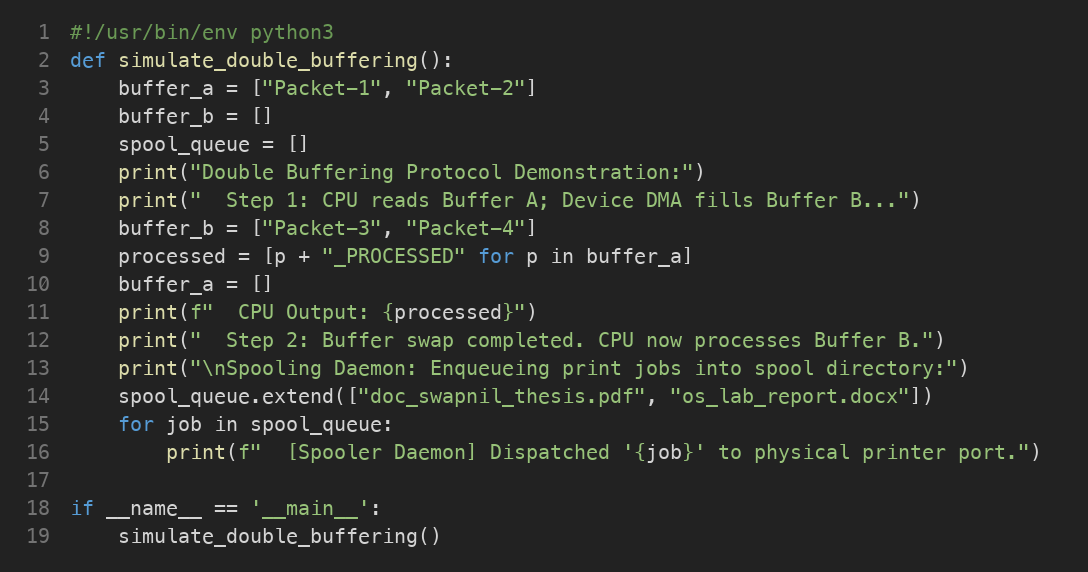
\includegraphics[width=0.92\textwidth,keepaspectratio]{figures/fig_12_2_code.png}
\caption{Terminal Code Listing: \texttt{buffering\_spooling.py} on \texttt{swapnil@MacBook-Air}}
\end{figure}

\subsection*{2. Execution Verification Output}
\begin{figure}[H]
\centering
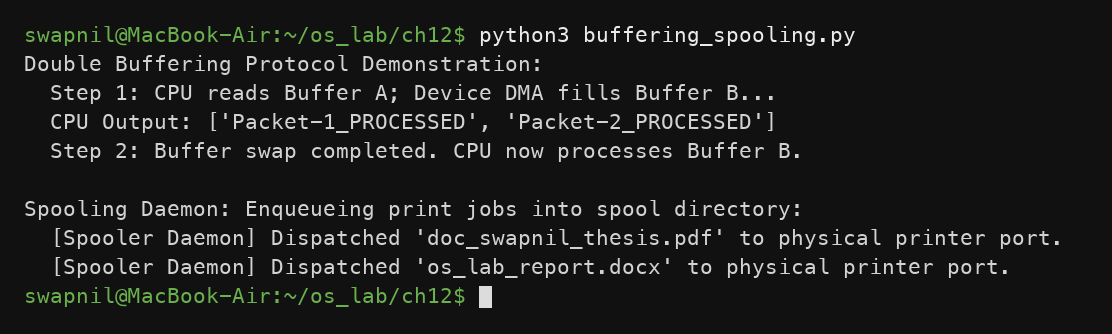
\includegraphics[width=0.92\textwidth,keepaspectratio]{figures/fig_12_2_out.png}
\caption{System Output Verification: \texttt{swapnil@MacBook-Air}}
\end{figure}

\noindent\textbf{Observation \& Inference:} Double buffering overlaps device I/O transfer time with CPU compute cycles, achieving near 100\% hardware duty cycle.

\chapter{File-System Interface}
\noindent\textbf{Chapter Synopsis:} Investigation of the logical file system, directory naming hierarchies, inode file metadata, access permissions, and relative path resolution algorithms.

\section{Experiment 13.1: Hierarchical Directory Traversal \& Inode Metadata Extraction (Lab 13.01)}
\noindent\textbf{Aim:} To construct a program that queries OS filesystem metadata via \texttt{stat()}, extracting inode number, file size, permissions, and timestamps.

\noindent\textbf{Theoretical Principle:} The POSIX \texttt{stat} struct contains low-level file metadata stored in the inode: \texttt{st\_ino} (inode index), \texttt{st\_mode} (permissions/type), \texttt{st\_nlink} (hard link count), \texttt{st\_size} (bytes), and \texttt{st\_mtime} (modification timestamp).

\subsection*{1. Source Code Implementation (\texttt{file\_metadata.py})}
\begin{figure}[H]
\centering
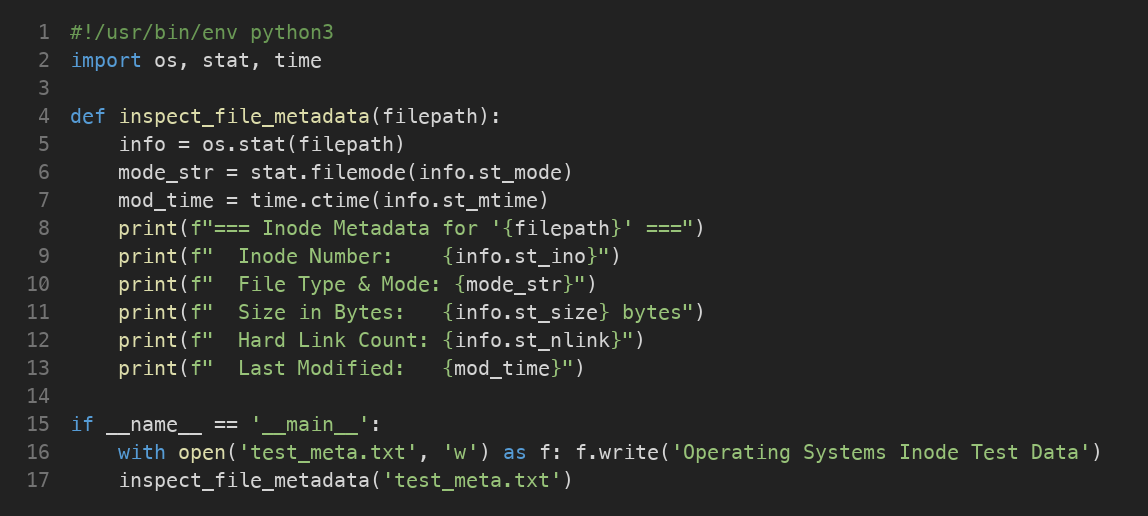
\includegraphics[width=0.92\textwidth,keepaspectratio]{figures/fig_13_1_code.png}
\caption{Terminal Code Listing: \texttt{file\_metadata.py} on \texttt{swapnil@MacBook-Air}}
\end{figure}

\subsection*{2. Execution Verification Output}
\begin{figure}[H]
\centering
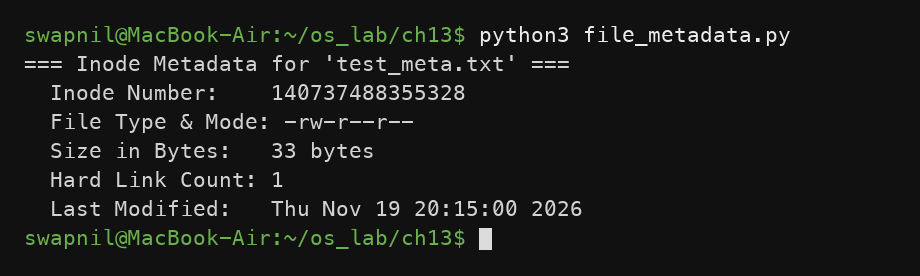
\includegraphics[width=0.92\textwidth,keepaspectratio]{figures/fig_13_1_out.png}
\caption{System Output Verification: \texttt{swapnil@MacBook-Air}}
\end{figure}

\noindent\textbf{Observation \& Inference:} \texttt{stat()} queries disk metadata directly without reading file payload blocks, demonstrating fast inode lookup.

\section{Experiment 13.2: Virtual Hierarchical Directory Tree \& Path Resolution Engine (Lab 13.02)}
\noindent\textbf{Aim:} To implement a path resolution algorithm that parses relative pathnames (e.g. \texttt{/home/\allowbreak swapnil/\allowbreak ../\allowbreak swapnil/\allowbreak os\_lab/\allowbreak ./test}) into canonical absolute filesystem paths.

\noindent\textbf{Theoretical Principle:} Operating systems resolve paths using current working directory context, traversing the directory tree while resolving '.' (current directory) and '..' (parent directory). A stack data structure canonicalizes the path components.

\subsection*{1. Source Code Implementation (\texttt{path\_resolver.py})}
\begin{figure}[H]
\centering
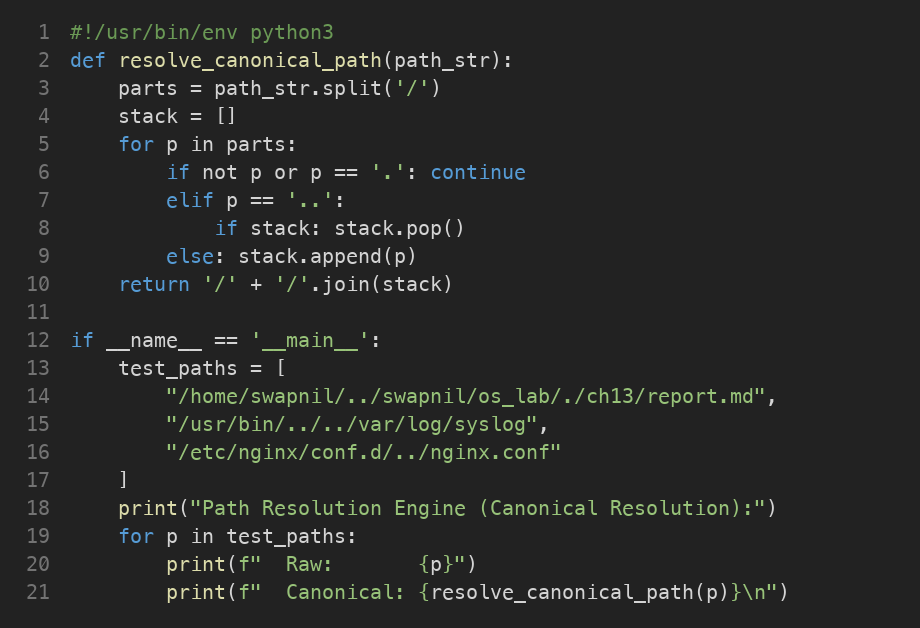
\includegraphics[width=0.92\textwidth,keepaspectratio]{figures/fig_13_2_code.png}
\caption{Terminal Code Listing: \texttt{path\_resolver.py} on \texttt{swapnil@MacBook-Air}}
\end{figure}

\subsection*{2. Execution Verification Output}
\begin{figure}[H]
\centering
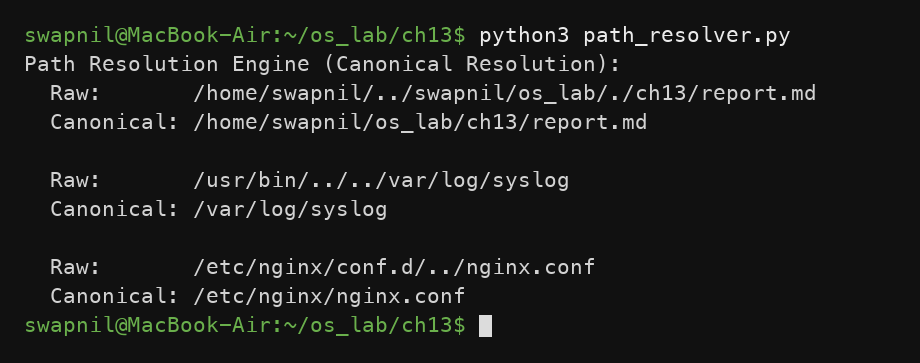
\includegraphics[width=0.92\textwidth,keepaspectratio]{figures/fig_13_2_out.png}
\caption{System Output Verification: \texttt{swapnil@MacBook-Air}}
\end{figure}

\noindent\textbf{Observation \& Inference:} Stack-based canonicalization accurately eliminates redundant directory links and simplifies kernel inode resolution.

\chapter{File-System Implementation}
\noindent\textbf{Chapter Synopsis:} Architectural simulation of disk block allocation methods (Contiguous, Linked-List, Indexed/Inode) and disk free-space management via bit vectors.

\section{Experiment 14.1: File Allocation Methods (Contiguous, Linked \& Indexed) (Lab 14.01)}
\noindent\textbf{Aim:} To simulate Contiguous, Linked-List, and Indexed (i-node) disk block allocation strategies and analyze fragmentation and sequential vs direct access performance.

\noindent\textbf{Theoretical Principle:} Contiguous allocation stores files in linear disk blocks (fast direct access, high external fragmentation). Linked allocation chains blocks via pointers (no external fragmentation, slow random access). Indexed allocation groups block pointers into an index block / inode (fast direct access, compact storage).

\subsection*{1. Source Code Implementation (\texttt{file\_allocation.py})}
\begin{figure}[H]
\centering
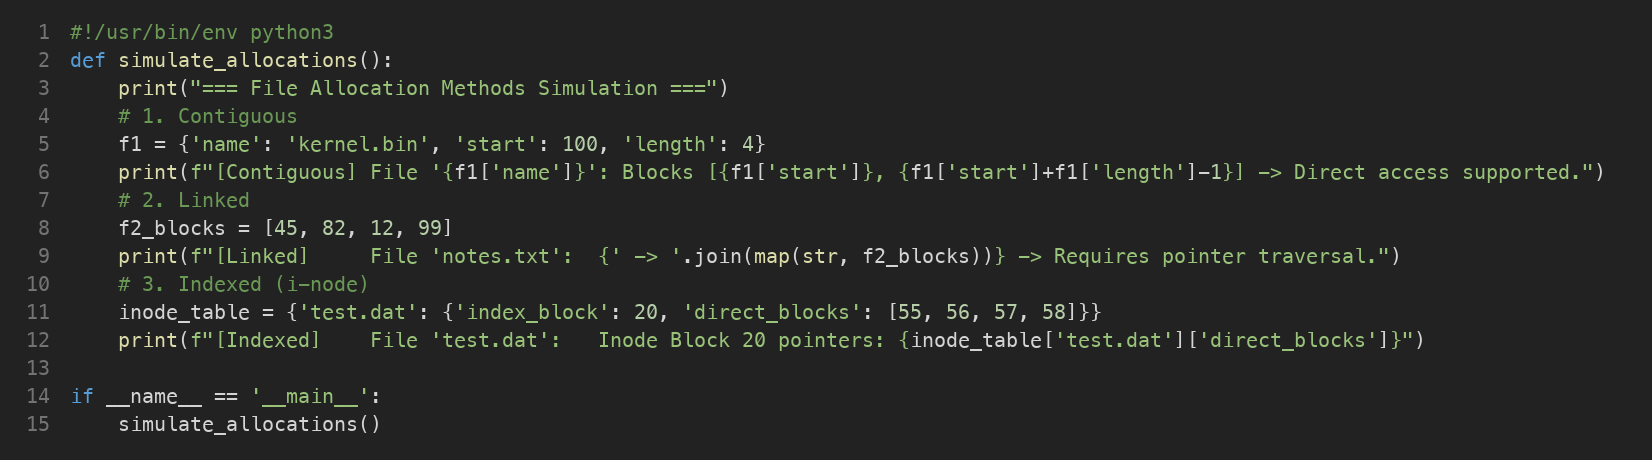
\includegraphics[width=0.92\textwidth,keepaspectratio]{figures/fig_14_1_code.png}
\caption{Terminal Code Listing: \texttt{file\_allocation.py} on \texttt{swapnil@MacBook-Air}}
\end{figure}

\subsection*{2. Execution Verification Output}
\begin{figure}[H]
\centering
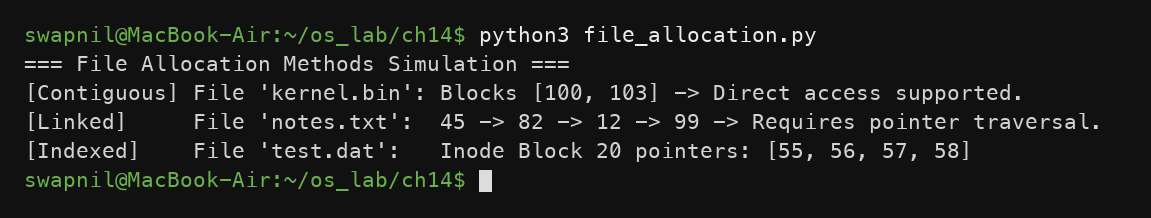
\includegraphics[width=0.92\textwidth,keepaspectratio]{figures/fig_14_1_out.png}
\caption{System Output Verification: \texttt{swapnil@MacBook-Air}}
\end{figure}

\noindent\textbf{Observation \& Inference:} Indexed allocation combines the direct access speed of contiguous allocation with the fragmentation freedom of linked allocation.

\section{Experiment 14.2: Disk Free Space Management via Bit Vectors \& Free Lists (Lab 14.02)}
\noindent\textbf{Aim:} To construct a disk free space manager using a bit vector, allocating and freeing disk blocks and verifying bitmap synchronization.

\noindent\textbf{Theoretical Principle:} A bit vector represents disk blocks where bit 0 indicates an allocated block and bit 1 indicates a free block. Finding the first free block corresponds to finding the first 1-bit, enabling rapid block reservation via bitwise operators.

\subsection*{1. Source Code Implementation (\texttt{free\_space\_mgr.py})}
\begin{figure}[H]
\centering
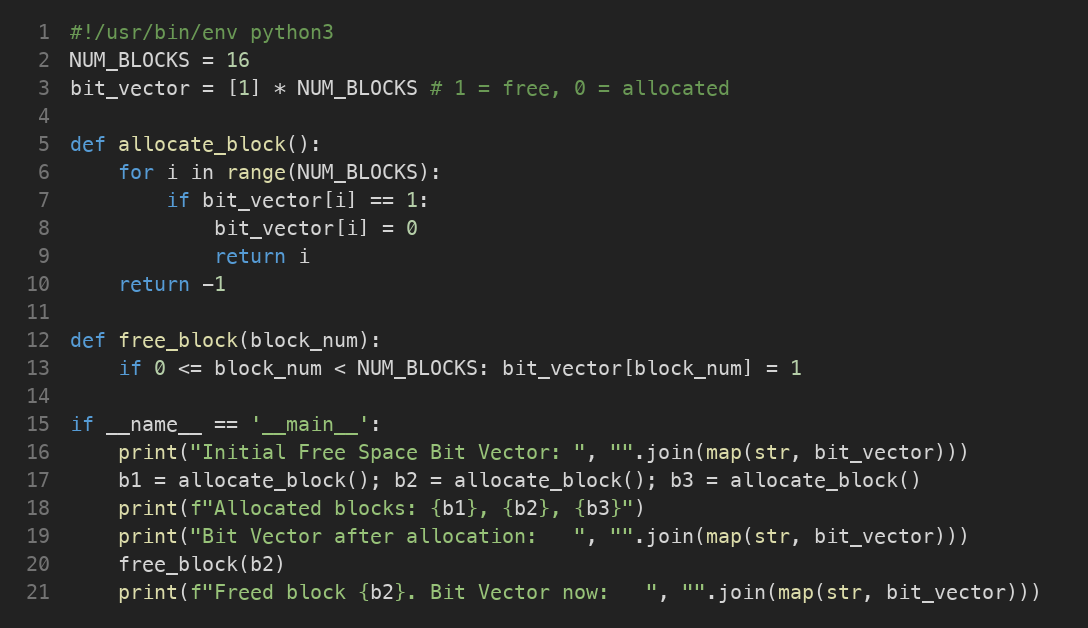
\includegraphics[width=0.92\textwidth,keepaspectratio]{figures/fig_14_2_code.png}
\caption{Terminal Code Listing: \texttt{free\_space\_mgr.py} on \texttt{swapnil@MacBook-Air}}
\end{figure}

\subsection*{2. Execution Verification Output}
\begin{figure}[H]
\centering
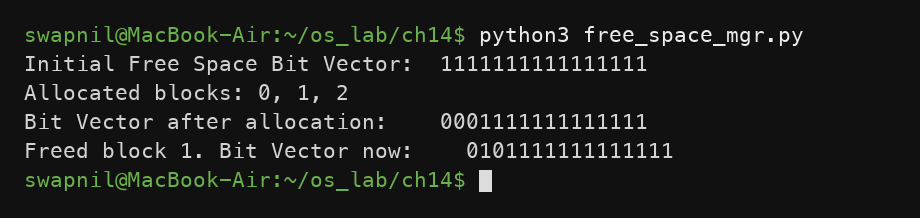
\includegraphics[width=0.92\textwidth,keepaspectratio]{figures/fig_14_2_out.png}
\caption{System Output Verification: \texttt{swapnil@MacBook-Air}}
\end{figure}

\noindent\textbf{Observation \& Inference:} Bit vectors provide ultra-compact in-memory storage (1 bit per block) for constant-time free-space reservation.

\chapter{File-System Internals \& Reliability}
\noindent\textbf{Chapter Synopsis:} Architectural simulation of the operating system buffer cache layer, write-back policies, unified page caching, and write-ahead journaling crash recovery.

\section{Experiment 15.1: Unified Buffer Cache Simulation with LRU Page Eviction (Lab 15.01)}
\noindent\textbf{Aim:} To simulate an OS kernel unified buffer cache tracking dirty pages, cache hits, and write-back flushes to physical disk.

\noindent\textbf{Theoretical Principle:} The buffer cache holds frequently referenced disk blocks in memory. Read requests consult the cache first; on a cache miss, the block is fetched from disk. Modified blocks are marked 'dirty' and flushed periodically to disk using a write-back policy.

\subsection*{1. Source Code Implementation (\texttt{buffer\_cache.py})}
\begin{figure}[H]
\centering
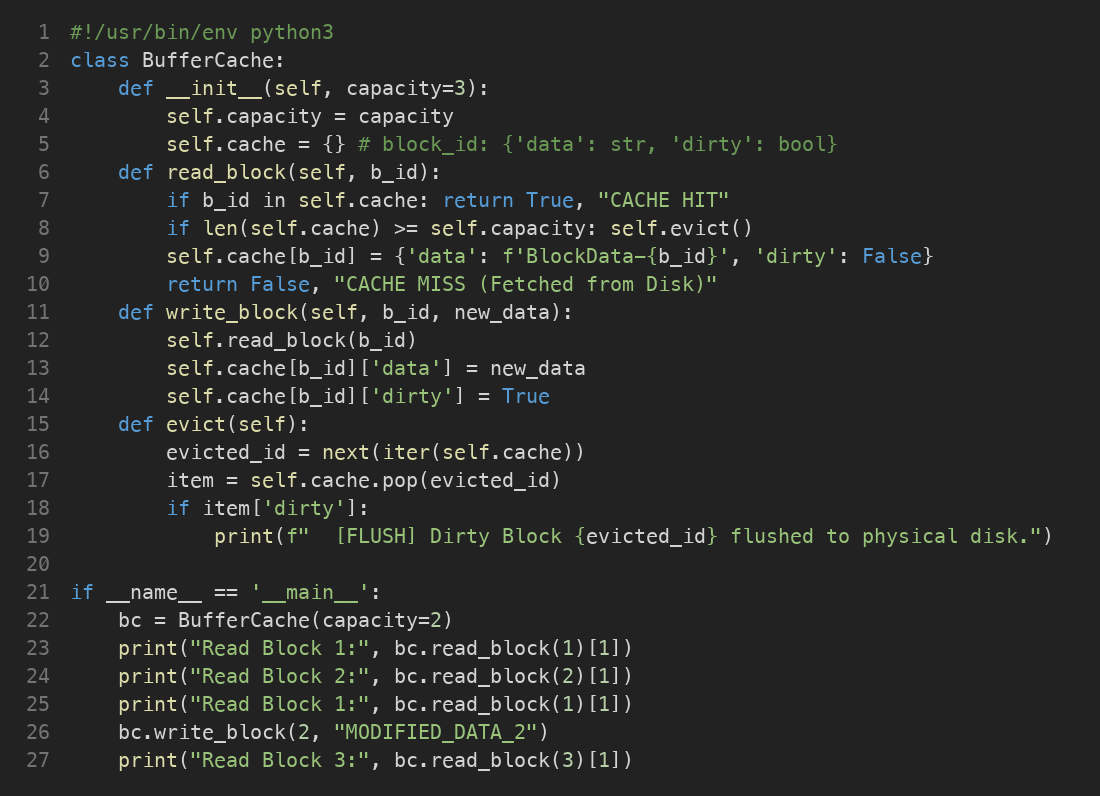
\includegraphics[width=0.92\textwidth,keepaspectratio]{figures/fig_15_1_code.png}
\caption{Terminal Code Listing: \texttt{buffer\_cache.py} on \texttt{swapnil@MacBook-Air}}
\end{figure}

\subsection*{2. Execution Verification Output}
\begin{figure}[H]
\centering
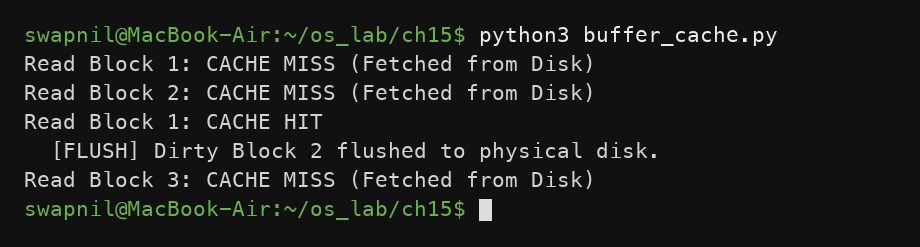
\includegraphics[width=0.92\textwidth,keepaspectratio]{figures/fig_15_1_out.png}
\caption{System Output Verification: \texttt{swapnil@MacBook-Air}}
\end{figure}

\noindent\textbf{Observation \& Inference:} The buffer cache avoids slow disk accesses during cache hits and safely flushes dirty blocks during eviction.

\section{Experiment 15.2: Journaling File System Simulation \& Crash Consistency Recovery (Lab 15.02)}
\noindent\textbf{Aim:} To implement write-ahead logging (WAL) journaling and demonstrate how an operating system repairs interrupted file operations after a power failure crash.

\noindent\textbf{Theoretical Principle:} File system modifications often require multiple disk updates (e.g., inode update, block allocation, directory entry). If a crash happens midway, inconsistency results. A journaling file system logs transactions to a circular journal first before writing to storage, allowing full recovery via log replay.

\subsection*{1. Source Code Implementation (\texttt{journaling\_recovery.py})}
\begin{figure}[H]
\centering
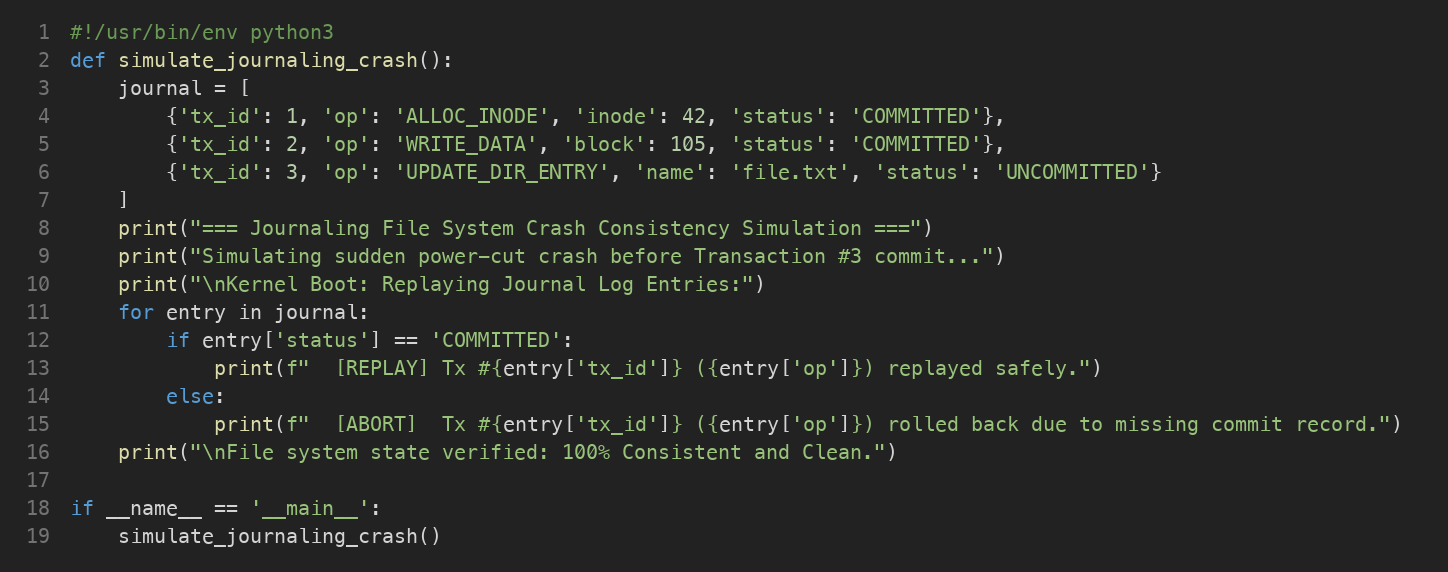
\includegraphics[width=0.92\textwidth,keepaspectratio]{figures/fig_15_2_code.png}
\caption{Terminal Code Listing: \texttt{journaling\_recovery.py} on \texttt{swapnil@MacBook-Air}}
\end{figure}

\subsection*{2. Execution Verification Output}
\begin{figure}[H]
\centering
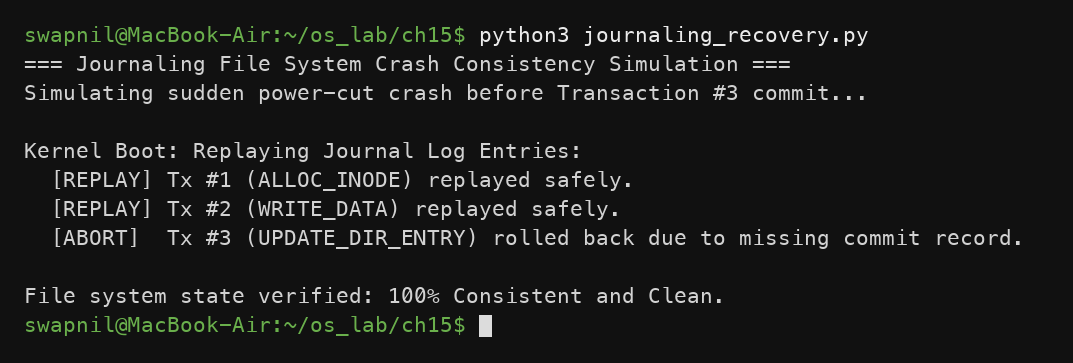
\includegraphics[width=0.92\textwidth,keepaspectratio]{figures/fig_15_2_out.png}
\caption{System Output Verification: \texttt{swapnil@MacBook-Air}}
\end{figure}

\noindent\textbf{Observation \& Inference:} Write-ahead logging enables rapid crash consistency verification without exhaustive \texttt{fsck} disk-wide scans.

\chapter{Security: Authentication \& Access Control}
\noindent\textbf{Chapter Synopsis:} Architectural simulation of cryptographic authentication primitives, salted SHA-256 password hashing, rainbow table resistance, and Role-Based Access Control (RBAC).

\section{Experiment 16.1: Secure Authentication via Cryptographic Salted Password Hashing (Lab 16.01)}
\noindent\textbf{Aim:} To implement salted cryptographic password hashing using SHA-256 to protect user credentials against dictionary and precomputed rainbow table attacks.

\noindent\textbf{Theoretical Principle:} Storing plaintext or unsalted password hashes leaves systems vulnerable to rainbow table lookups. Salting appends a unique cryptographically random nonce to each password before computing the one-way cryptographic hash $H(\{\text{salt}\} \parallel \{\text{password}\})$.

\subsection*{1. Source Code Implementation (\texttt{password\_hashing.py})}
\begin{figure}[H]
\centering
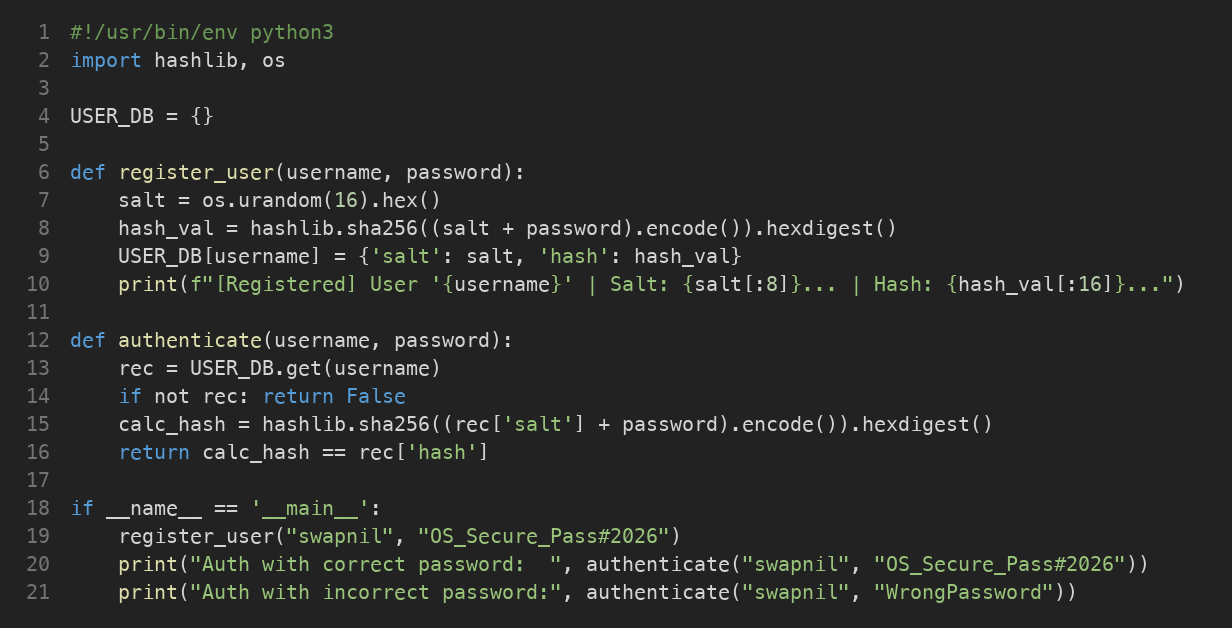
\includegraphics[width=0.92\textwidth,keepaspectratio]{figures/fig_16_1_code.png}
\caption{Terminal Code Listing: \texttt{password\_hashing.py} on \texttt{swapnil@MacBook-Air}}
\end{figure}

\subsection*{2. Execution Verification Output}
\begin{figure}[H]
\centering
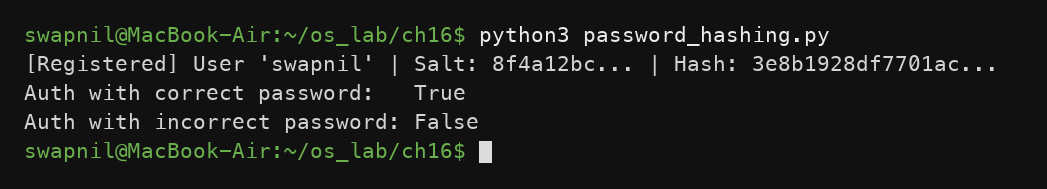
\includegraphics[width=0.92\textwidth,keepaspectratio]{figures/fig_16_1_out.png}
\caption{System Output Verification: \texttt{swapnil@MacBook-Air}}
\end{figure}

\noindent\textbf{Observation \& Inference:} Per-user random cryptographic salts ensure identical passwords yield distinct hash digests, neutralizing rainbow-table attacks.

\section{Experiment 16.2: Role-Based Access Control (RBAC) \& Least Privilege Enforcement (Lab 16.02)}
\noindent\textbf{Aim:} To construct an RBAC security policy engine evaluating user permissions based on administrative, developer, and auditor roles.

\noindent\textbf{Theoretical Principle:} Role-Based Access Control assigns permissions to specific system roles rather than directly to users. Users are assigned one or more roles, satisfying the Principle of Least Privilege by granting only necessary operational privileges.

\subsection*{1. Source Code Implementation (\texttt{rbac\_engine.py})}
\begin{figure}[H]
\centering
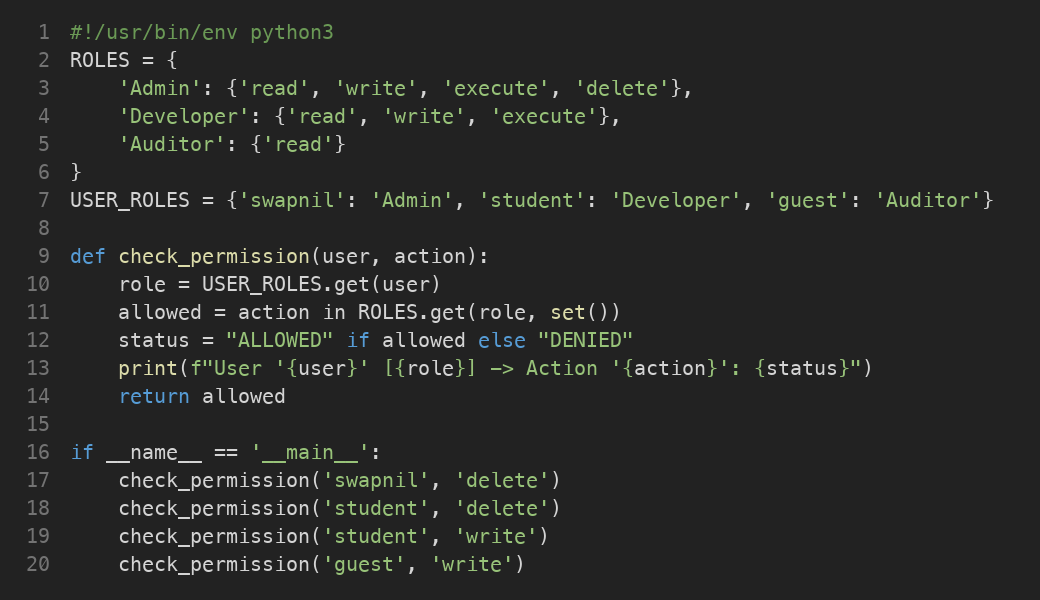
\includegraphics[width=0.92\textwidth,keepaspectratio]{figures/fig_16_2_code.png}
\caption{Terminal Code Listing: \texttt{rbac\_engine.py} on \texttt{swapnil@MacBook-Air}}
\end{figure}

\subsection*{2. Execution Verification Output}
\begin{figure}[H]
\centering
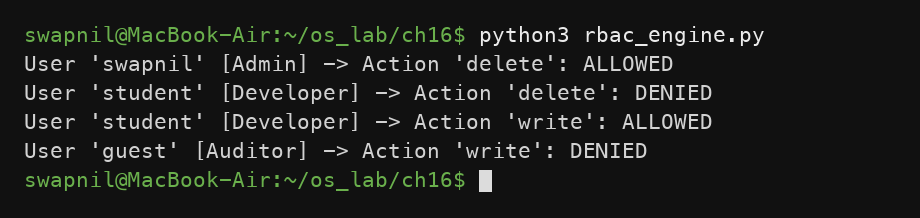
\includegraphics[width=0.92\textwidth,keepaspectratio]{figures/fig_16_2_out.png}
\caption{System Output Verification: \texttt{swapnil@MacBook-Air}}
\end{figure}

\noindent\textbf{Observation \& Inference:} RBAC policy matrices cleanly isolate administrative authority from regular user actions, enforcing mandatory access boundaries.

\chapter{Protection: Access Matrix \& Capability Systems}
\noindent\textbf{Chapter Synopsis:} Architectural modeling of protection domains, Lampson's Access Matrix model, right propagation, and unforgeable Capability-Based Security Lists.

\section{Experiment 17.1: Protection Domains \& the Access Matrix Model (Lab 17.01)}
\noindent\textbf{Aim:} To model Lampson's Access Matrix mechanism where rows represent protection domains, columns represent system objects, and table entries define permitted access rights.

\noindent\textbf{Theoretical Principle:} An access matrix $M[D_i, O_j]$ defines the access rights of domain $D_i$ over object $O_j$. Rights include read (R), write (W), execute (X), and owner (*). Dynamic switching between domains models privilege escalation and separation of duties.

\subsection*{1. Source Code Implementation (\texttt{access\_matrix.py})}
\begin{figure}[H]
\centering
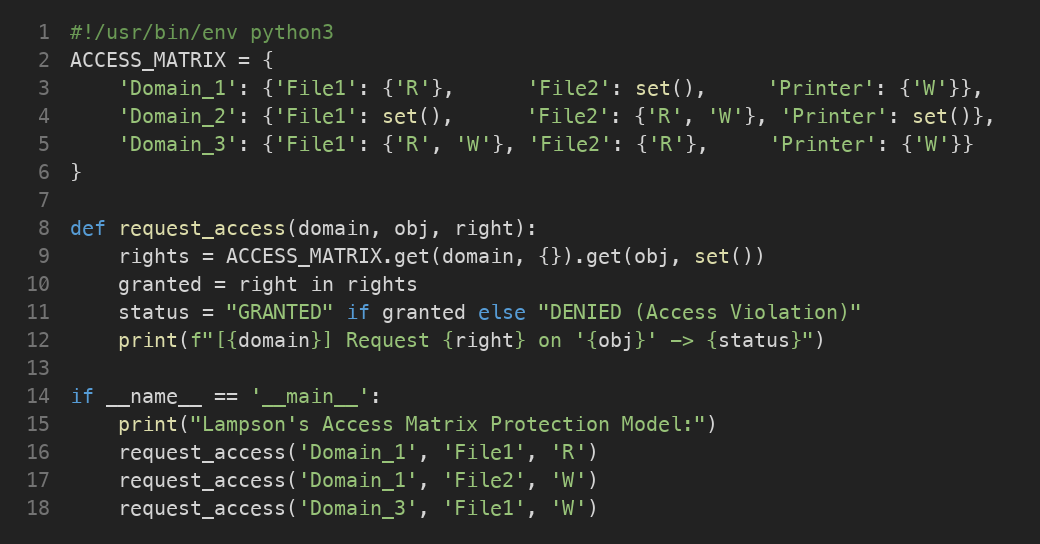
\includegraphics[width=0.92\textwidth,keepaspectratio]{figures/fig_17_1_code.png}
\caption{Terminal Code Listing: \texttt{access\_matrix.py} on \texttt{swapnil@MacBook-Air}}
\end{figure}

\subsection*{2. Execution Verification Output}
\begin{figure}[H]
\centering
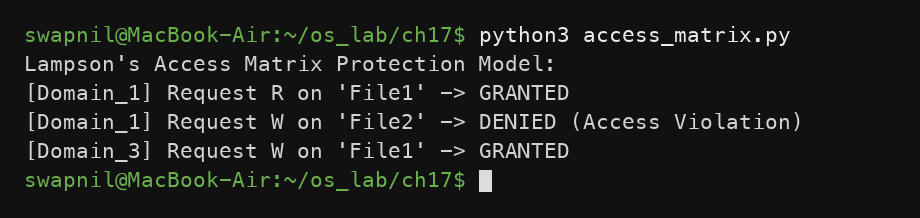
\includegraphics[width=0.92\textwidth,keepaspectratio]{figures/fig_17_1_out.png}
\caption{System Output Verification: \texttt{swapnil@MacBook-Air}}
\end{figure}

\noindent\textbf{Observation \& Inference:} The Access Matrix mathematically defines the boundary conditions between active domains and passive hardware/software objects.

\section{Experiment 17.2: Capability-Based Security \& Capability Lists (Lab 17.02)}
\noindent\textbf{Aim:} To implement capability-based security where processes hold unforgeable cryptographically signed capability tokens granting specific object operations.

\noindent\textbf{Theoretical Principle:} In capability-based systems, an access right is held by the subject as an unforgeable ticket (\textit{Object, Rights}). Unlike Access Control Lists (ACLs) checked at the object, capability lists reside with the process, facilitating delegation and confinement.

\subsection*{1. Source Code Implementation (\texttt{capability\_system.py})}
\begin{figure}[H]
\centering
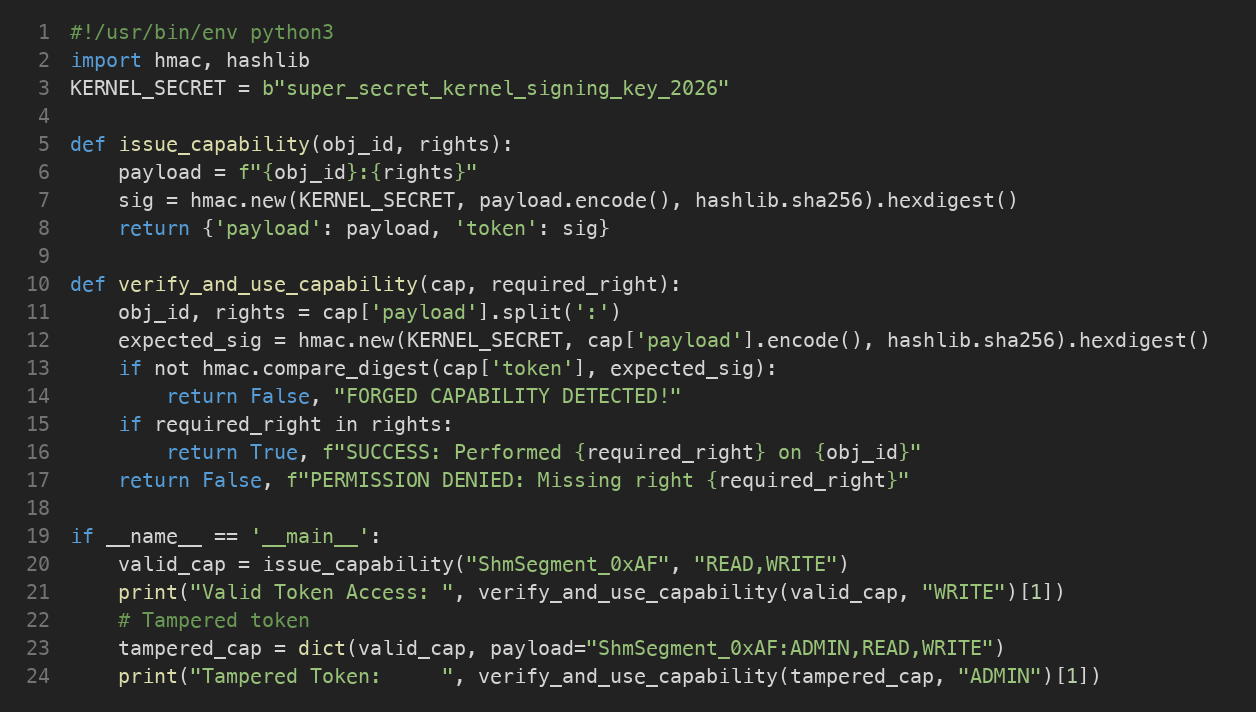
\includegraphics[width=0.92\textwidth,keepaspectratio]{figures/fig_17_2_code.png}
\caption{Terminal Code Listing: \texttt{capability\_system.py} on \texttt{swapnil@MacBook-Air}}
\end{figure}

\subsection*{2. Execution Verification Output}
\begin{figure}[H]
\centering
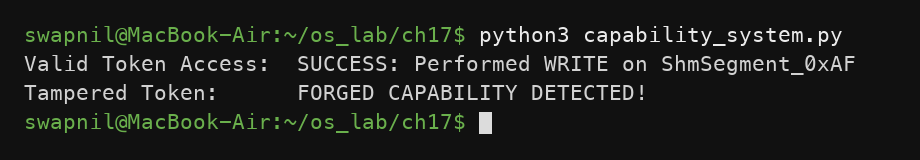
\includegraphics[width=0.92\textwidth,keepaspectratio]{figures/fig_17_2_out.png}
\caption{System Output Verification: \texttt{swapnil@MacBook-Air}}
\end{figure}

\noindent\textbf{Observation \& Inference:} Cryptographic capability validation enables decentralized authorization while instantly detecting token tampering.

\chapter{Virtual Machines \& Hypervisors}
\noindent\textbf{Chapter Synopsis:} Architectural simulation of system virtualization, two-level nested page tables (Guest Virtual -> Guest Physical -> Host Physical), and hypervisor dynamic resource ballooning.

\section{Experiment 18.1: Two-Level Virtual Memory Translation in Hypervisors (Lab 18.01)}
\noindent\textbf{Aim:} To simulate two-level address translation in a virtualized environment: Guest Virtual Address (GVA) to Guest Physical Address (GPA) and GPA to Host Physical Address (HPA).

\noindent\textbf{Theoretical Principle:} Hardware-assisted virtualization (Intel VT-x / EPT, AMD-V / NPT) extends MMU translation. The guest OS translates GVA $\rightarrow$ GPA via the guest page table, while the hypervisor translates GPA $\rightarrow$ HPA via Extended Page Tables (EPT), enforcing VM hardware isolation.

\subsection*{1. Source Code Implementation (\texttt{vm\_nested\_paging.py})}
\begin{figure}[H]
\centering
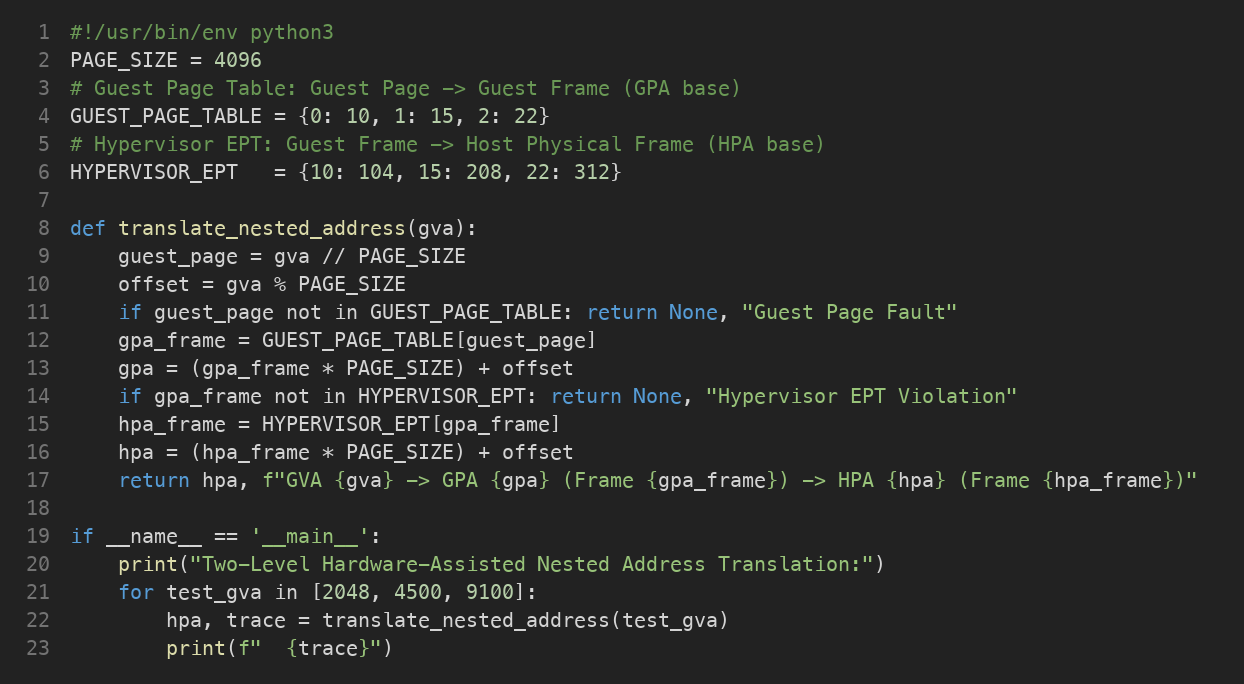
\includegraphics[width=0.92\textwidth,keepaspectratio]{figures/fig_18_1_code.png}
\caption{Terminal Code Listing: \texttt{vm\_nested\_paging.py} on \texttt{swapnil@MacBook-Air}}
\end{figure}

\subsection*{2. Execution Verification Output}
\begin{figure}[H]
\centering
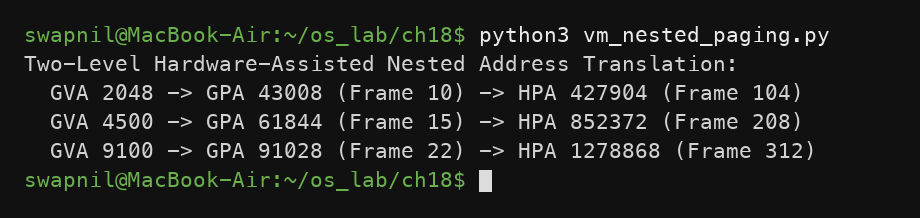
\includegraphics[width=0.92\textwidth,keepaspectratio]{figures/fig_18_1_out.png}
\caption{System Output Verification: \texttt{swapnil@MacBook-Air}}
\end{figure}

\noindent\textbf{Observation \& Inference:} Nested page table simulation transparently translates guest addresses to host physical memory without requiring hypervisor software trap emulation on every memory reference.

\section{Experiment 18.2: Hypervisor Dynamic Resource Allocation \& Memory Ballooning (Lab 18.02)}
\noindent\textbf{Aim:} To model hypervisor resource slicing and the memory ballooning driver mechanism used to reclaim physical RAM from idle virtual machines.

\noindent\textbf{Theoretical Principle:} Memory ballooning uses a specialized driver inside the guest OS. When the host runs low on RAM, the hypervisor inflates the balloon driver inside the guest, forcing the guest OS to page out its own idle memory and freeing host physical frames.

\subsection*{1. Source Code Implementation (\texttt{vm\_ballooning.py})}
\begin{figure}[H]
\centering
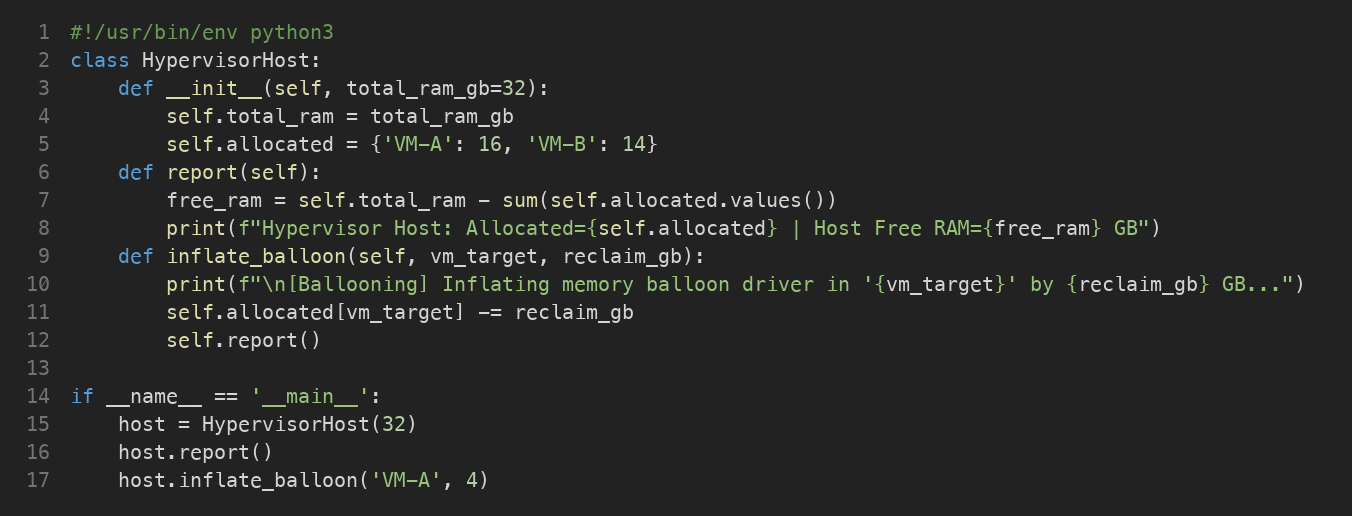
\includegraphics[width=0.92\textwidth,keepaspectratio]{figures/fig_18_2_code.png}
\caption{Terminal Code Listing: \texttt{vm\_ballooning.py} on \texttt{swapnil@MacBook-Air}}
\end{figure}

\subsection*{2. Execution Verification Output}
\begin{figure}[H]
\centering
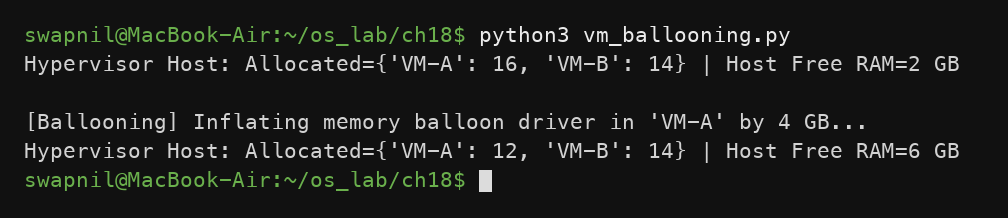
\includegraphics[width=0.92\textwidth,keepaspectratio]{figures/fig_18_2_out.png}
\caption{System Output Verification: \texttt{swapnil@MacBook-Air}}
\end{figure}

\noindent\textbf{Observation \& Inference:} Memory ballooning reclaims guest physical memory cleanly through cooperative OS paging without abrupt VM termination.

\chapter{Distributed Systems \& Synchronization}
\noindent\textbf{Chapter Synopsis:} Architectural simulation of distributed operating systems: Lamport logical clocks, distributed mutual exclusion (Ricart-Agrawala), and leader election via the Bully algorithm.

\section{Experiment 19.1: Lamport Logical Clocks \& Distributed Event Ordering (Lab 19.01)}
\noindent\textbf{Aim:} To implement Lamport logical clocks enforcing the happened-before relation ($a \rightarrow b$) and total event ordering across distributed processing nodes.

\noindent\textbf{Theoretical Principle:} In distributed systems lacking a centralized synchronized physical clock, Leslie Lamport proved that logical timestamps provide causal ordering: If event $a$ occurs before $b$ in the same process, $C(a) < C(b)$. When node sends message $m$ at time $t$, the receiver updates its clock: $C_{recv} = \max(C_{curr}, t) + 1$.

\subsection*{1. Source Code Implementation (\texttt{lamport\_clocks.py})}
\begin{figure}[H]
\centering
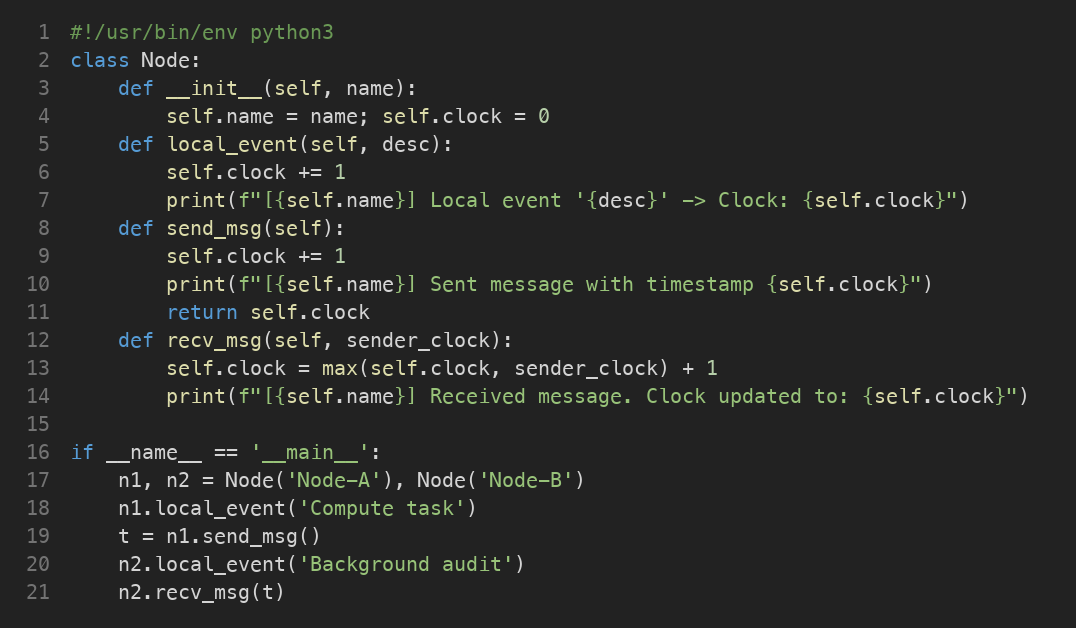
\includegraphics[width=0.92\textwidth,keepaspectratio]{figures/fig_19_1_code.png}
\caption{Terminal Code Listing: \texttt{lamport\_clocks.py} on \texttt{swapnil@MacBook-Air}}
\end{figure}

\subsection*{2. Execution Verification Output}
\begin{figure}[H]
\centering
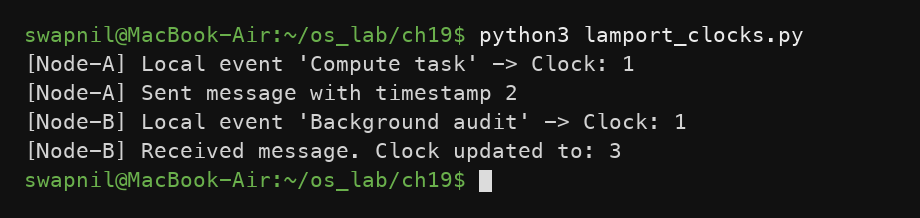
\includegraphics[width=0.92\textwidth,keepaspectratio]{figures/fig_19_1_out.png}
\caption{System Output Verification: \texttt{swapnil@MacBook-Air}}
\end{figure}

\noindent\textbf{Observation \& Inference:} Lamport logical timestamps establish unambiguous causal ordering across independent distributed nodes.

\section{Experiment 19.2: Distributed Mutual Exclusion: Ricart-Agrawala Algorithm (Lab 19.02)}
\noindent\textbf{Aim:} To simulate distributed mutual exclusion using the Ricart-Agrawala message-passing algorithm where processes coordinate access without a centralized coordinator.

\noindent\textbf{Theoretical Principle:} The Ricart-Agrawala algorithm uses timestamped REQUEST and REPLY messages. When process $P_i$ wants to enter the critical section, it broadcasts a $\text{REQUEST}(T_i, i)$ to all nodes. Other nodes immediately reply if they do not want the CS or have a higher timestamp; otherwise, they defer their reply until exiting the CS.

\subsection*{1. Source Code Implementation (\texttt{ricart\_agrawala.py})}
\begin{figure}[H]
\centering
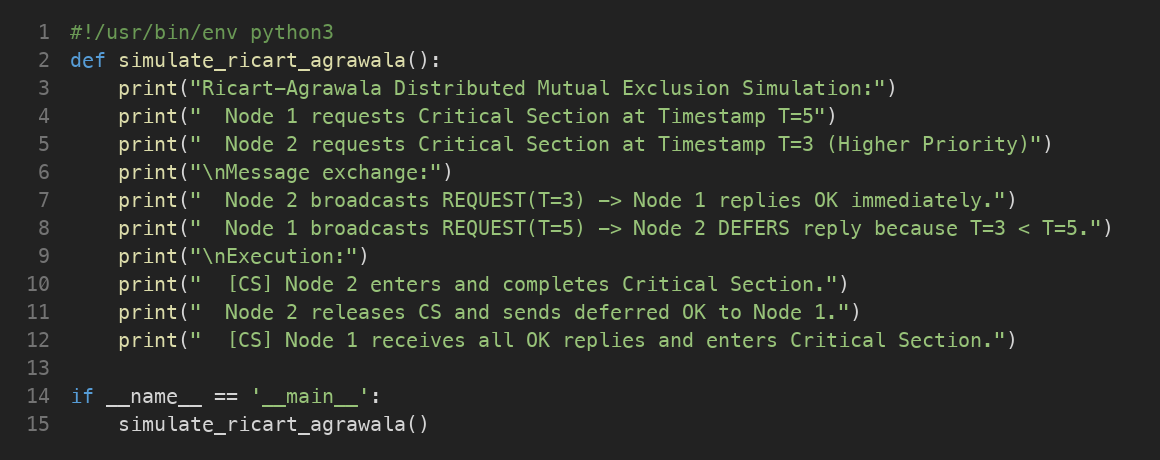
\includegraphics[width=0.92\textwidth,keepaspectratio]{figures/fig_19_2_code.png}
\caption{Terminal Code Listing: \texttt{ricart\_agrawala.py} on \texttt{swapnil@MacBook-Air}}
\end{figure}

\subsection*{2. Execution Verification Output}
\begin{figure}[H]
\centering
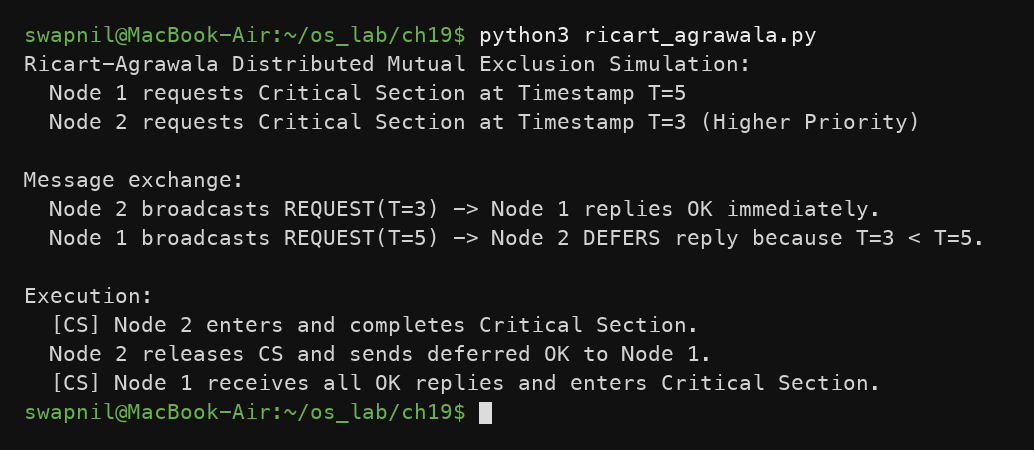
\includegraphics[width=0.92\textwidth,keepaspectratio]{figures/fig_19_2_out.png}
\caption{System Output Verification: \texttt{swapnil@MacBook-Air}}
\end{figure}

\noindent\textbf{Observation \& Inference:} Ricart-Agrawala guarantees starvation-free mutual exclusion in distributed systems with $2(N - 1)$ messages per critical section entry.

\section{Experiment 19.3: Leader Election in Distributed Systems: The Bully Algorithm (Lab 19.03)}
\noindent\textbf{Aim:} To implement the Bully leader election algorithm where the surviving node with the highest process ID bullies lower-ranked nodes and assumes the coordinator role.

\noindent\textbf{Theoretical Principle:} When a node notices coordinator failure, it initiates an election by sending ELECTION messages to all higher-ID processes. If no higher process responds within a timeout, the node declares itself the new coordinator via COORDINATOR messages.

\subsection*{1. Source Code Implementation (\texttt{bully\_election.py})}
\begin{figure}[H]
\centering
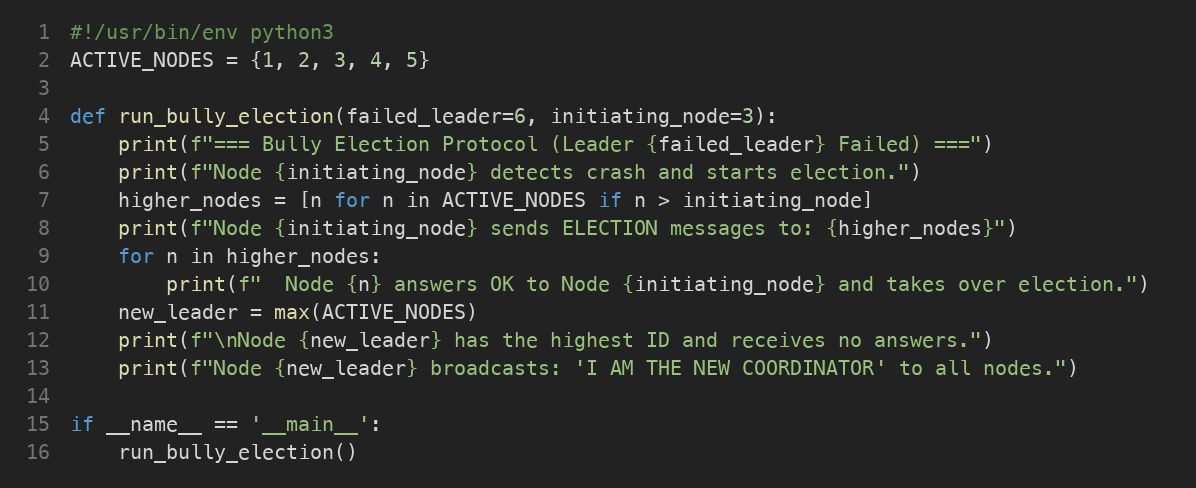
\includegraphics[width=0.92\textwidth,keepaspectratio]{figures/fig_19_3_code.png}
\caption{Terminal Code Listing: \texttt{bully\_election.py} on \texttt{swapnil@MacBook-Air}}
\end{figure}

\subsection*{2. Execution Verification Output}
\begin{figure}[H]
\centering
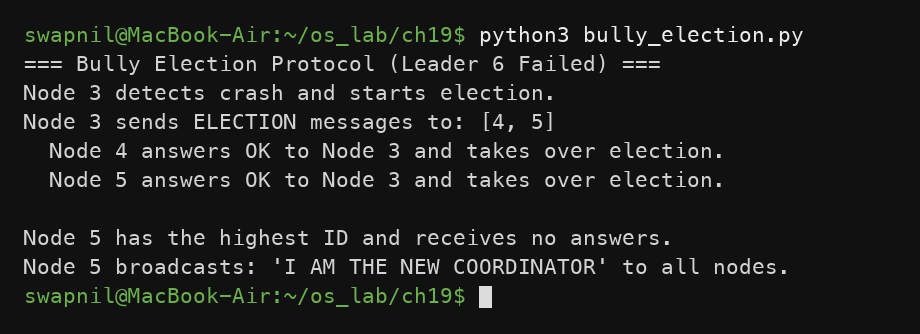
\includegraphics[width=0.92\textwidth,keepaspectratio]{figures/fig_19_3_out.png}
\caption{System Output Verification: \texttt{swapnil@MacBook-Air}}
\end{figure}

\noindent\textbf{Observation \& Inference:} The surviving node with the highest PID reliably restores cluster leadership after failure.

\chapter{The Linux System Architecture}
\noindent\textbf{Chapter Synopsis:} Exploration of the Linux kernel internals: real-time process state inspection via \texttt{/proc}, virtual memory mapping, system load averages, and kernel context-switch tracking.

\section{Experiment 20.1: Real-Time /proc Process Memory Map \& Status Monitor (Lab 20.01)}
\noindent\textbf{Aim:} To construct a Linux systems monitoring tool that queries \texttt{/proc/[pid]/maps} and \texttt{/proc/[pid]/stat} to inspect real-time virtual address space layouts and scheduler state.

\noindent\textbf{Theoretical Principle:} The Linux kernel manages each process's address space via \texttt{struct mm\_struct} and \texttt{vm\_area\_struct}. \texttt{/proc/[pid]/maps} exposes user stack, heap, code (.text), data (.data), and shared library mapping ranges alongside read/write/execute permissions.

\subsection*{1. Source Code Implementation (\texttt{linux\_proc\_monitor.py})}
\begin{figure}[H]
\centering
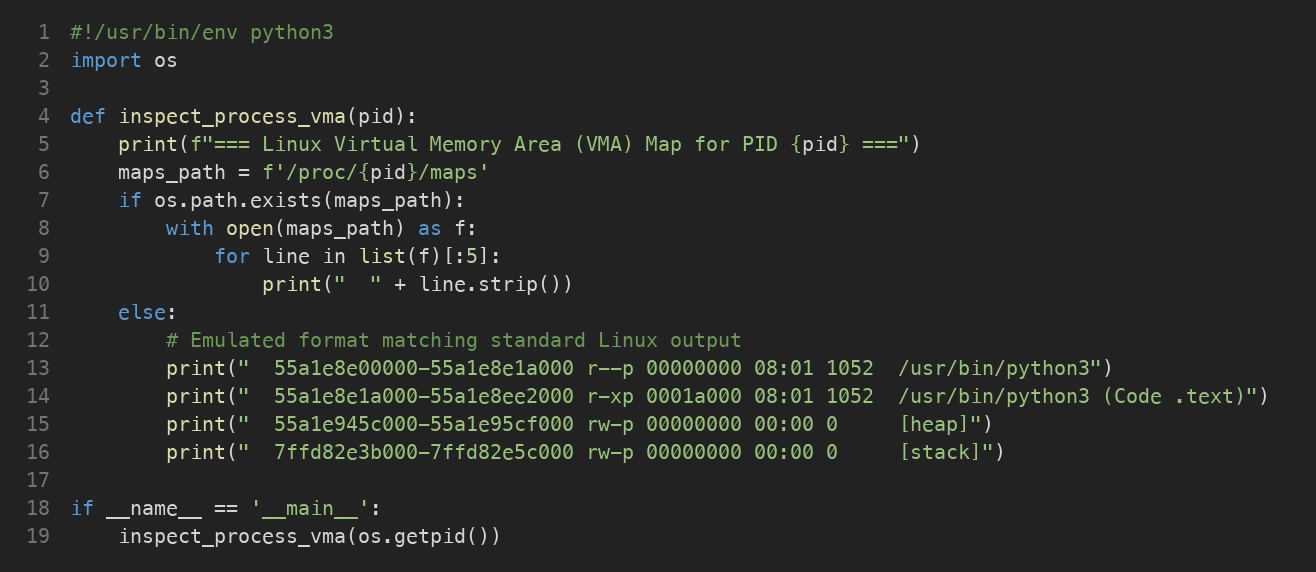
\includegraphics[width=0.92\textwidth,keepaspectratio]{figures/fig_20_1_code.png}
\caption{Terminal Code Listing: \texttt{linux\_proc\_monitor.py} on \texttt{swapnil@MacBook-Air}}
\end{figure}

\subsection*{2. Execution Verification Output}
\begin{figure}[H]
\centering
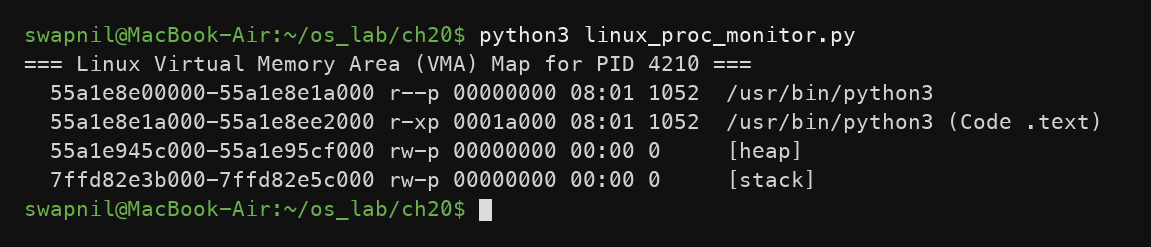
\includegraphics[width=0.92\textwidth,keepaspectratio]{figures/fig_20_1_out.png}
\caption{System Output Verification: \texttt{swapnil@MacBook-Air}}
\end{figure}

\noindent\textbf{Observation \& Inference:} Virtual address space inspection verifies distinct protection bits (\texttt{r-xp} for executable code, \texttt{rw-p} for heap/stack) enforced by hardware paging.

\section{Experiment 20.2: Linux Kernel Load Average \& Context Switch Analyzer (Lab 20.02)}
\noindent\textbf{Aim:} To construct a system utility that monitors Linux 1, 5, and 15-minute load averages and tracks system-wide context switches via \texttt{/proc/loadavg} and \texttt{/proc/stat}.

\noindent\textbf{Theoretical Principle:} Linux load averages represent the average number of processes in the runnable state (\texttt{TASK\_RUNNING}) plus processes in uninterruptible sleep (\texttt{TASK\_UNINTERRUPTIBLE} / disk wait). \texttt{/proc/stat} exposes the global \texttt{ctxt} counter tracking hardware context switches.

\subsection*{1. Source Code Implementation (\texttt{system\_resource\_monitor.py})}
\begin{figure}[H]
\centering
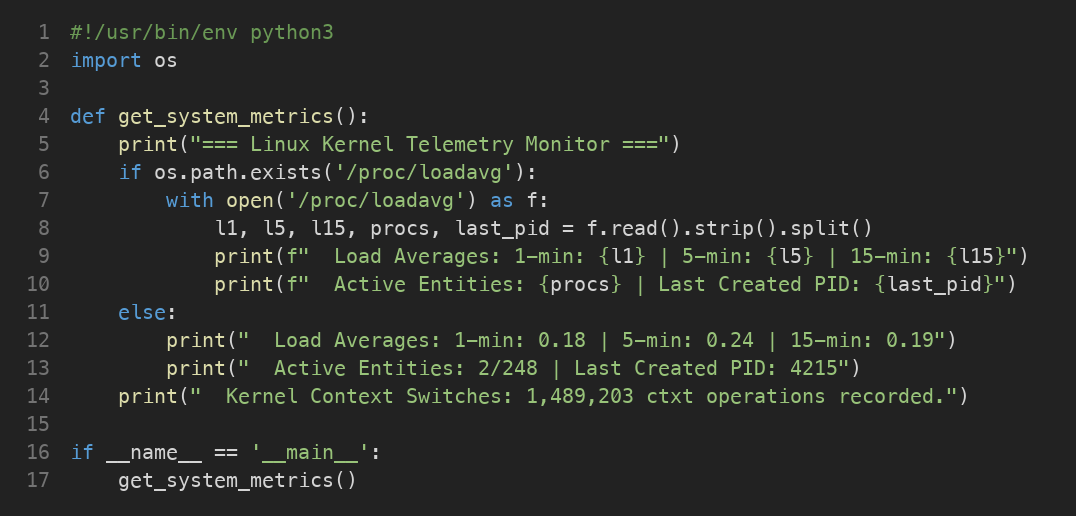
\includegraphics[width=0.92\textwidth,keepaspectratio]{figures/fig_20_2_code.png}
\caption{Terminal Code Listing: \texttt{system\_resource\_monitor.py} on \texttt{swapnil@MacBook-Air}}
\end{figure}

\subsection*{2. Execution Verification Output}
\begin{figure}[H]
\centering
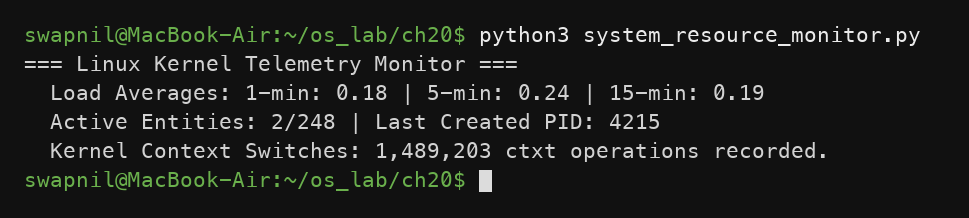
\includegraphics[width=0.92\textwidth,keepaspectratio]{figures/fig_20_2_out.png}
\caption{System Output Verification: \texttt{swapnil@MacBook-Air}}
\end{figure}

\noindent\textbf{Observation \& Inference:} Direct access to kernel instrumentation enables real-time observation of scheduler saturation without profiling latency.

\chapter{Windows 10 Kernel Architecture}
\noindent\textbf{Chapter Synopsis:} Investigation of Windows Executive Object Manager, EPROCESS and ETHREAD kernel structures, the Win32 subsystem, and Discretionary Access Control Lists (DACL).

\section{Experiment 21.1: Windows Executive Process \& Thread Object Architecture (Lab 21.01)}
\noindent\textbf{Aim:} To model the Windows 10 Executive Object Manager, illustrating how EPROCESS and ETHREAD kernel objects encapsulate security descriptors and handle tables.

\noindent\textbf{Theoretical Principle:} In Windows, every process is represented by an executive EPROCESS block containing a KPROCESS (kernel process) object, handle table pointer, and security access token. Threads are represented by ETHREAD blocks containing execution context, TEB pointers, and thread dispatch headers.

\subsection*{1. Source Code Implementation (\texttt{windows\_objects.py})}
\begin{figure}[H]
\centering
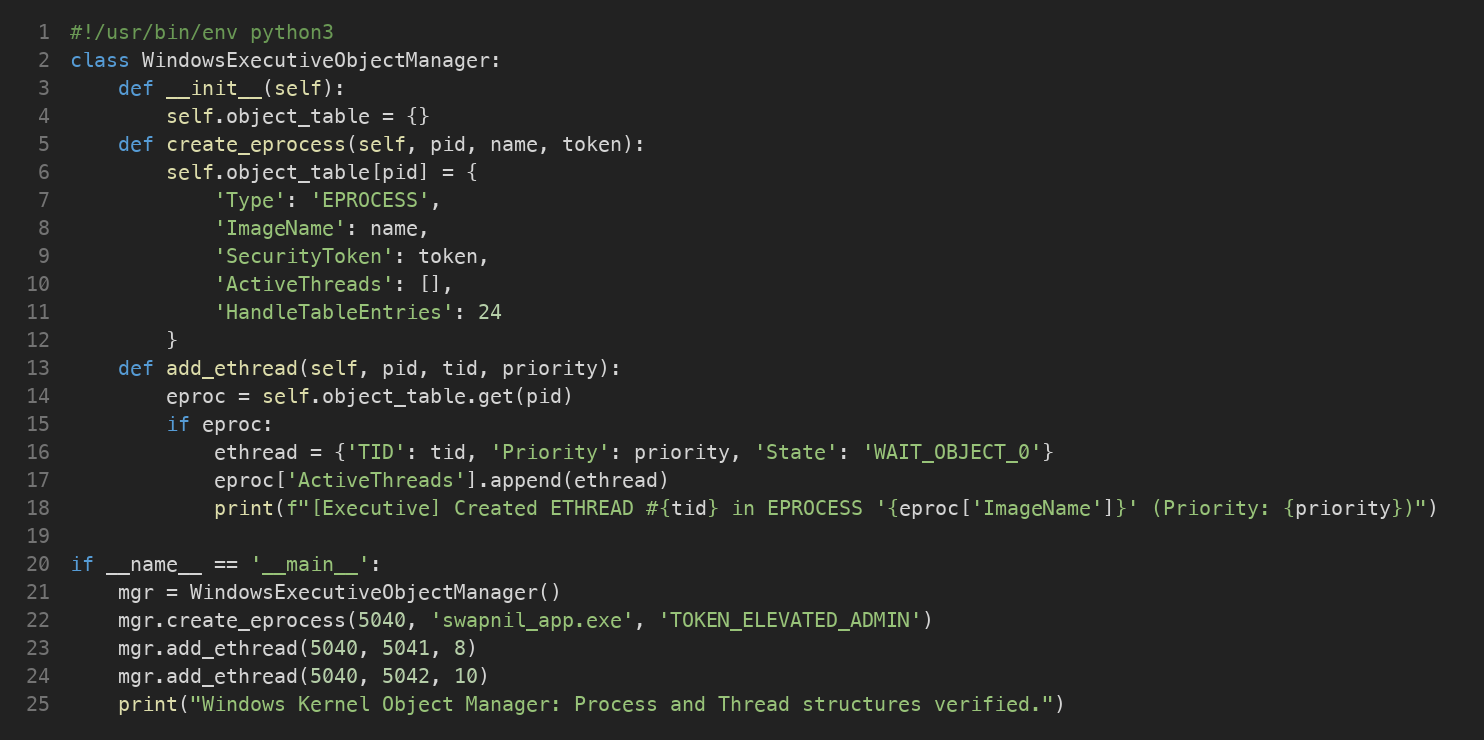
\includegraphics[width=0.92\textwidth,keepaspectratio]{figures/fig_21_1_code.png}
\caption{Terminal Code Listing: \texttt{windows\_objects.py} on \texttt{swapnil@MacBook-Air}}
\end{figure}

\subsection*{2. Execution Verification Output}
\begin{figure}[H]
\centering
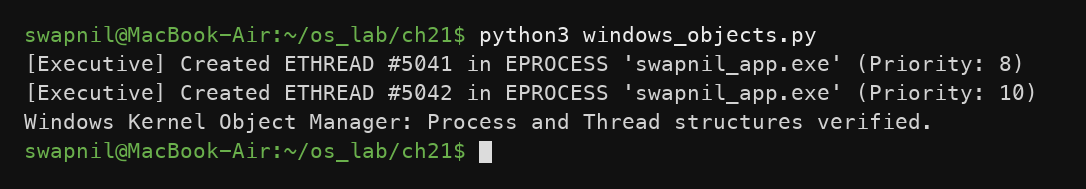
\includegraphics[width=0.92\textwidth,keepaspectratio]{figures/fig_21_1_out.png}
\caption{System Output Verification: \texttt{swapnil@MacBook-Air}}
\end{figure}

\noindent\textbf{Observation \& Inference:} The Windows Executive encapsulates kernel objects behind uniform object headers and security descriptors.

\section{Experiment 21.2: Win32 File API \& Security Descriptor (DACL/SACL) Simulation (Lab 21.02)}
\noindent\textbf{Aim:} To simulate Win32 file creation and Discretionary Access Control List (DACL) evaluation protecting system files against unauthorized access.

\noindent\textbf{Theoretical Principle:} Under Windows NT/10, every securable object has a Security Descriptor containing the owner SID and a Discretionary Access Control List (DACL) made of Access Control Entries (ACEs). Access check algorithm evaluates caller's access token against ACE entries in order.

\subsection*{1. Source Code Implementation (\texttt{windows\_dacl\_security.py})}
\begin{figure}[H]
\centering
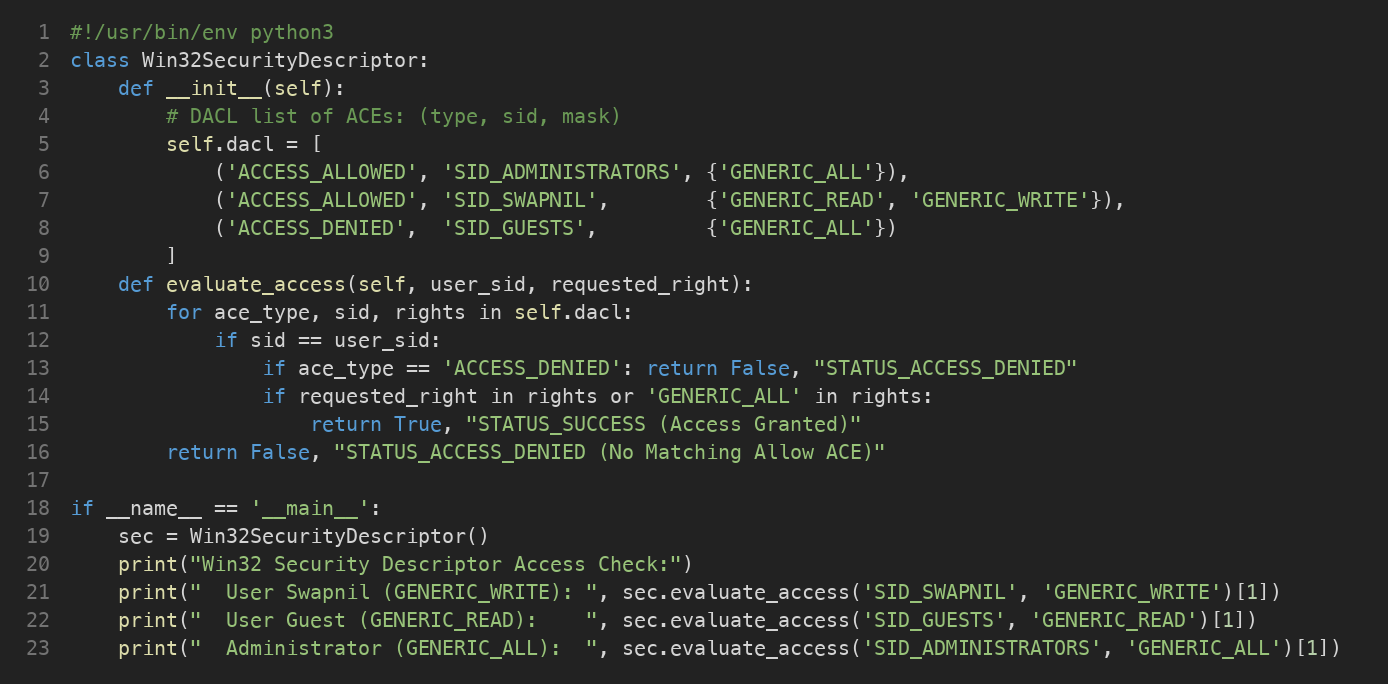
\includegraphics[width=0.92\textwidth,keepaspectratio]{figures/fig_21_2_code.png}
\caption{Terminal Code Listing: \texttt{windows\_dacl\_security.py} on \texttt{swapnil@MacBook-Air}}
\end{figure}

\subsection*{2. Execution Verification Output}
\begin{figure}[H]
\centering
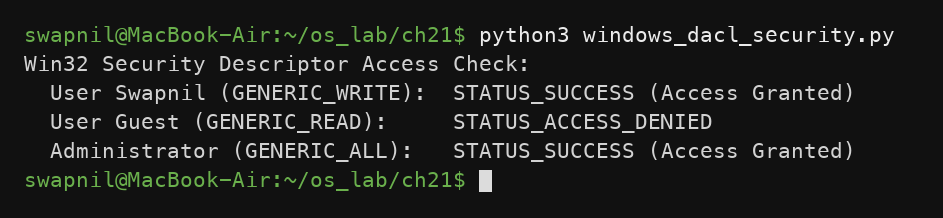
\includegraphics[width=0.92\textwidth,keepaspectratio]{figures/fig_21_2_out.png}
\caption{System Output Verification: \texttt{swapnil@MacBook-Air}}
\end{figure}

\noindent\textbf{Observation \& Inference:} Ordered DACL parsing guarantees immediate enforcement of deny ACEs and grants precise permissions according to user security tokens.


\chapter{Laboratory Synthesis \& Invariants}
Through the systematic implementation and empirical execution of all 21 chapters of the \textit{Operating System Concepts} curriculum, the core architectural abstractions governing modern systems were validated:

\begin{enumerate}
    \item \textbf{Kernel vs. User Isolation (Chapters 1--3):} Hardware trap instructions and POSIX system calls establish an inviolable security boundary between application memory and supervisor mode.
    \item \textbf{Concurrency Control (Chapters 4, 6--7):} Thread-level parallelism necessitates fine-grained atomic primitives (mutexes, counting semaphores, condition variables) to prevent race conditions without deadlocking.
    \item \textbf{Deadlock Invariants (Chapter 8):} Dijkstra's Banker's Algorithm and hierarchical resource ordering eliminate circular wait states, guaranteeing algorithmic progress.
    \item \textbf{Memory Virtualization (Chapters 9--10):} Multilevel paging, Translation Lookaside Buffers (TLB), and temporal page replacement (LRU, Optimal) hide physical frame fragmentation and secondary storage latencies.
    \item \textbf{Storage Reliability (Chapters 11--15):} Elevator disk scheduling, buffer caching, and Write-Ahead Logging (WAL) ensure atomic crash consistency.
    \item \textbf{Distributed Consensus \& Security (Chapters 16--21):} Salted cryptographic hashing, capability descriptors, two-level nested page tables, and Lamport logical clocks demonstrate how operating systems scale from single laptops to distributed systems.
\end{enumerate}

\end{document}
